\documentclass[a4paper,12pt]{article}
\usepackage [utf8x]{inputenc}
\usepackage[czech]{babel}
\usepackage{graphicx}
\usepackage{amsmath}
\usepackage{siunitx}
\usepackage{xspace}
\usepackage{url}
\usepackage{indentfirst}
\usepackage[margin=22mm]{geometry}
\usepackage{esvect}
\usepackage{ragged2e}
\usepackage{tikz,pgf}
\usepackage{bm}
\usepackage{perpage}
\usepackage{capt-of}
\usepackage{subcaption}

\graphicspath{
	{img/}
	{plots/}
	{plots/2ndderivates/}
	{plots/poruchove/}
}

\newcommand{\e}{\text{e}}


\MakeSorted{figure}
\newtoks\jmenopraktika \newtoks\jmeno \newtoks\datum
\newtoks\obor \newtoks\skupina \newtoks\rocnik \newtoks\semestr
\newtoks\cisloulohy \newtoks\jmenoulohy
\newtoks\tlak \newtoks\teplota \newtoks\vlhkost
\jmenopraktika={Diagnostika plazmatu doutnavého výboje pomocí jednoduché sondy}  % nahradte jmenem vaseho predmetu
\jmeno={Radek Horňák, Lukáš Vrána}            
\datum={1. 3. 2022}        % nahradte datem mereni ulohy                           
\rocnik={2.}                  
\semestr={IV.}                 
\cisloulohy={6}    % cislo ulohy           

\begin{document}
	\begin{center}
		{\Large Přírodovědecká fakulta Masarykovy univerzity} \\
		\bigskip
		{\Large \bfseries PRAKTIKUM Z~FYZIKY PLAZMATU} \\
		\bigskip
		{\Large \the\jmenopraktika}
	\end{center}
	\bigskip
	\noindent
	\setlength{\arrayrulewidth}{1pt}
	\begin{tabular*}{\textwidth}{@{\extracolsep{\fill}} l l}
		\large {\bfseries Zpracovali:}  \the\jmeno  \hspace{20mm} \large  
		{\bfseries Naměřeno:} \the\datum\\[2.5mm]
		\hline
	\end{tabular*}

\section{Teorie}
%\subsection{Doutnavý výboj}
%V této úloze se budeme zabývat měřením parametrů kladného sloupce doutnavého výboje.	
%Doutnavý výboj je druh výboje, jehož typický vzhled můžeme vidět na schématu na 
%obr.~\ref{glow+napeti}. V~rozmezí tlaku 10$^1$-10$^2$\,\si{\pascal} v~něm můžeme 
%pozorovat střídající se temné nebo svítící místa, která rozlišujeme na katodové a anodové oblasti. Katodové oblasti jsou nutnou a důležitou oblastí doutnavého výboje na rozdíl od kladného sloupce, jehož délka se při zkracování vzdálenosti elektrod zmenšuje a může i úplně zmizet. Intenzita elektrického pole je podél jeho osy konstantní, viz dolní část obr. \ref{glow+napeti}. Může být určena buď pomocí sondových měření nebo ji lze vypočítat ze závislosti napětí na elektrodách na jejich vzdálenosti při konstantním proudu ve výboji.

%\begin{figure}[h]
%	\centering
%	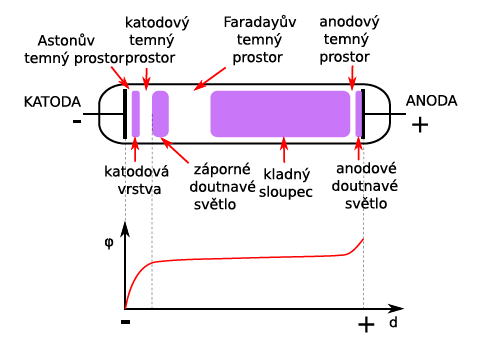
\includegraphics[width=110mm]{glow+napeti.png}
%	\caption{Doutnavý výboj a intenzita elektrického pole podíl jeho osy}
%	\label{glow+napeti}
%\end{figure}

\subsection{Elektrostatická Langmuirova sonda}
Langmuirova sonda je vodič malých rozměrů zavedený do plazmatu, pomocí nějž lze měřit
nejdůležitější parametry plazmatu jako elektronovou hustotu $n_\text{e}$, teplotu elektronů~$T_\text{e}$, rozdělovací funkci elektronů $f(v)$ a prostorové rozdělení potenciálu a
elektrického pole. Napětí sondy $V_\text{S}$ určujeme vzhledem k referenční elektrodě. Potenciál 
plazmatu v místě sondy vůči stejné referenční elektrodě označme $V_\text{p}$. Pokud je vůči ní 
plocha sondy velmi malá, můžeme sondu nazvat jednoduchou. Podle tvaru lze dále sondy dělit na 
válcové, kulové a~rovinné. Závislost proudu protékajícího sondou $I_\text{S}$ na napětí 
přiloženém na sondu $V_\text{S}$ tvoří volt\-am\-pé\-ro\-vou (VA) charakteristiku sondy. Napětí 
sondy vůči plazmovému potenciálu $U_\text{S}$ získáme pomocí vztahu

\begin{equation}
	U_\text{S} = V_\text{S} - V_\text{p}
	\label{Usondy}
\end{equation}
Pokud sonda není připojena k vnějšímu obvodu a proud elektronů i iontů na ni se ustálí, je výsledný proud nulový a sonda se ustálí na napětí $V_\text{{fl}}$, tedy na plovoucím potenciálu.

VA charakteristiku jednoduché sondy můžeme rozdělit na tři části. Tou první je oblast saturovaného iontového proudu označená na obr.
\ref{VA} jako $A$. Sonda je záporně nabita vzhledem k potenciálu plazmatu, elektrony jsou odpuzovány a ionty naopak přitahovány. Vizuálně se to projevuje temným prostorem obalujícím sondu.

Druhou část charakteristiky tvoří přechodová oblast, pro kterou lze 
$U_\text{S}$ vymezit jako $-2 (V_\text{p} - V_\text{{fl}}) \leq
U_\text{S} \leq 0$. Na obr. \ref{VA} se jedná o oblast $B$. Celkový proud 
sondou $I_\text{S}$ můžeme vyjádřit jako

\begin{equation}
	I_\text{S} = I_\text{i} + I_\text{e}
\end{equation}
kde $I_\text{i}$ je iontový proud a $I_\text{e}$ elektronový proud, který je dán vztahem

\begin{equation}
	I_\text{e} = S e n_\text{e} \sqrt{\frac{k T_\text{e}}{2 \pi m_\text{e}}} \exp \left(\frac{-eU_\text{S}}{k T_\text{e}}\right)
	\label{eproud}
\end{equation}
kde $S$ je povrch sondy, $e$ elementární náboj, $n_\text{e}$ koncentrace elektronů, $k$ Boltzmanova konstanta a $m_\text{e}$ hmotnost
elektronu.

Oblast saturovaného elektronového proudu je na obr. \ref{VA} označená jako $C$. Sonda je vzhledem k potenciálu plazmatu na kladném
napětí a přitahuje tak elektrony. U válcové sondy nejeví tato oblast nasycení, nýbrž parabolicky narůstá.


\begin{figure}[h]
	\centering
	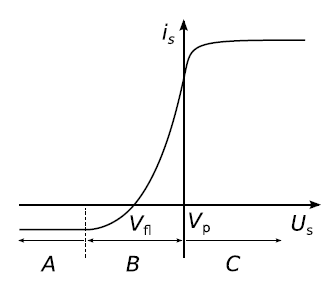
\includegraphics[width=90mm]{VA.png}
	\caption{VA charakteristika jednoduché rovinné sondy \cite{VA}.}
	\label{VA}
\end{figure}	
\subsection{Rozdělovací funkce energie}
V předchozí části předpokládáme Maxwellovo rozdělení energie elektronů.
Zdali tento předpoklad platí lze dokázat Druyvesteynovým vztahem:
\begin{equation}
	f(\vert U_s\vert) = 
	\frac{1}{A}\sqrt{\left(\frac{8m_\text{e}}{e^3}\right)} \sqrt{\vert 
	U_s\vert} \frac{\text{d}^2i_\text{e}}{\text{d}U^2_\text{s}}
\label{Druyvesteyn}
\end{equation}
Existuje několik metod, jak získat ze sondové charakteristiky funkci 
$\frac{\text{d}^2i_\text{e}}{\text{d}U^2_\text{s}}$, která udává 
roz\-dě\--lo\-va\-cí 
funkci. Jednou z %možností je numerická derivace. Druhou 
možností je přiložení 
slabého střídavého napětí 
$U=\varepsilon\sin(\omega t)$, přičemž musí platit 
$\varepsilon/U_\text{s}\ll1$. Složka stejnosměrného proudu sondy vzroste o 
hodnotu 
\begin{equation}
\Delta i \approx 
\frac{\varepsilon^2}{4}\frac{\text{d}^2i_\text{e}}{\text{d}U^2_\text{s}}
\label{delta i}
\end{equation}
Rozdělovací funkce $f(\vert U_s\vert)$ je tedy úměrná $\sqrt{\vert 
U_s\vert}\Delta i$. Tuto závislost graficky zobrazíme a lze ji porovnat s 
obecnými předpisy Maxwellova a Druyvesteynova rozdělení

\begin{equation}
	f(E) = A \sqrt{E} \exp \left[ -\left( \frac{E}{B} \right)^K \right]
	\label{eq:rozdeleni}
\end{equation}
s parametry $A,B,K$. Pokud je $K=1$, jedná se o Maxwellovo rozdělení, v případě 
$K=2$ je rozdělení Druyvesteynovo.

\newpage
\section{Měření a výsledky}
Měření provádíme na aparatuře, jejíž schéma je vidět na obr. \ref{schema}. Výbojka je čerpaná rotační olejovou vývěvou. Tlak
nastavujeme změnou průtoku argonu a měříme jej Piraniho manometrem. Do výbojky je zavedená jednoduchá válcová sonda, jejíž délku jsme
odhadli na 8 \si{\milli\meter} a průměr 0,1 \si{\milli\meter}. Povrch podstavy válcové sondy je k povrchu jejího pláště $S$~zanedbatelný, po zaokrouhlení dostáváme $S = 2,5\cdot10^{-6}$ \si{\meter\squared}. 

Při měření vždy nejprve nalezneme plovoucí potenciál, abychom měli jistotu, že naměříme oblast 
nalevo i napravo od něj. Napětí přiložené na sondu $V_\text{S}$ se mění automaticky pomocí 
potenciometru, který je poháněn elektrickým motorkem, kde stačí zařadit rychlostní stupeň v jednom
ze směrů chodu. Data jsou ukládána na počítač. Při vyhodnocování jsme je museli 
synchronizovat. VA charakteristiku jsme naměřili v obou směrech chodu 
potenciometru. Tato data se mezi sebou mírně lišila. Pro následné zpracování 
jsme použili vždy data pouze jednoho směru.

\begin{figure}[h]
	\centering
	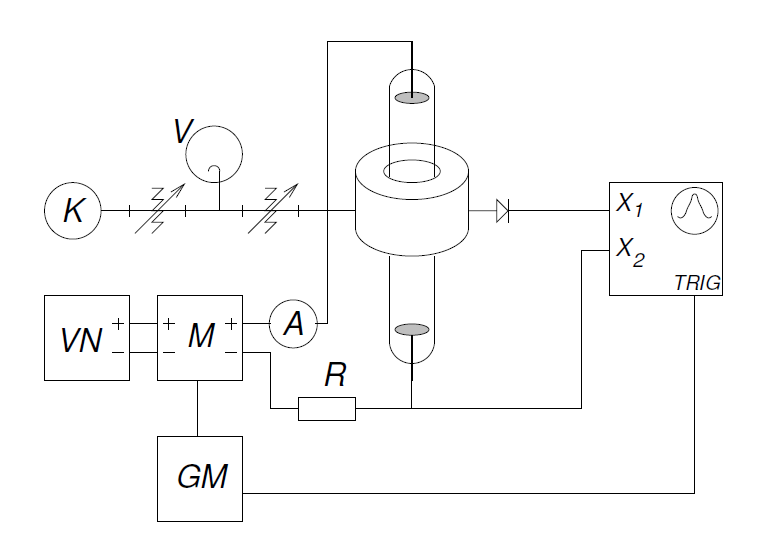
\includegraphics[width=120mm]{schema.png}
	\caption{Schéma aparatury \cite{VA}.}
	\label{schema}
\end{figure}

Provedli jsme měření za konstantního tlaku 160 \si{\pascal} pro tři hodnoty výbojového proudu~$I_\text{v}$. Výsledné VA charakteristiky
jsou v grafu na obr. \ref{namerene012}. Z nich lze určit plovoucí potenciál, který se s rostoucím výbojovým proudem zvětšuje, viz tab.
\ref{tab1}. Dále jsme provedli měření za konstantního výbojového proudu 40 \si{\milli\ampere} pro pět hodnot tlaku. Odpovídající VA
charakteristiky jsou v grafu na obr. \ref{namerene34567}. Pro tlak 320 \si{\pascal} je plovoucí potenciál nejmenší, v oblasti 8--80
\si{\pascal} však nevykazuje žádný trend, viz tab. \ref{tab1}.

\begin{figure}[h!]
	\centering
	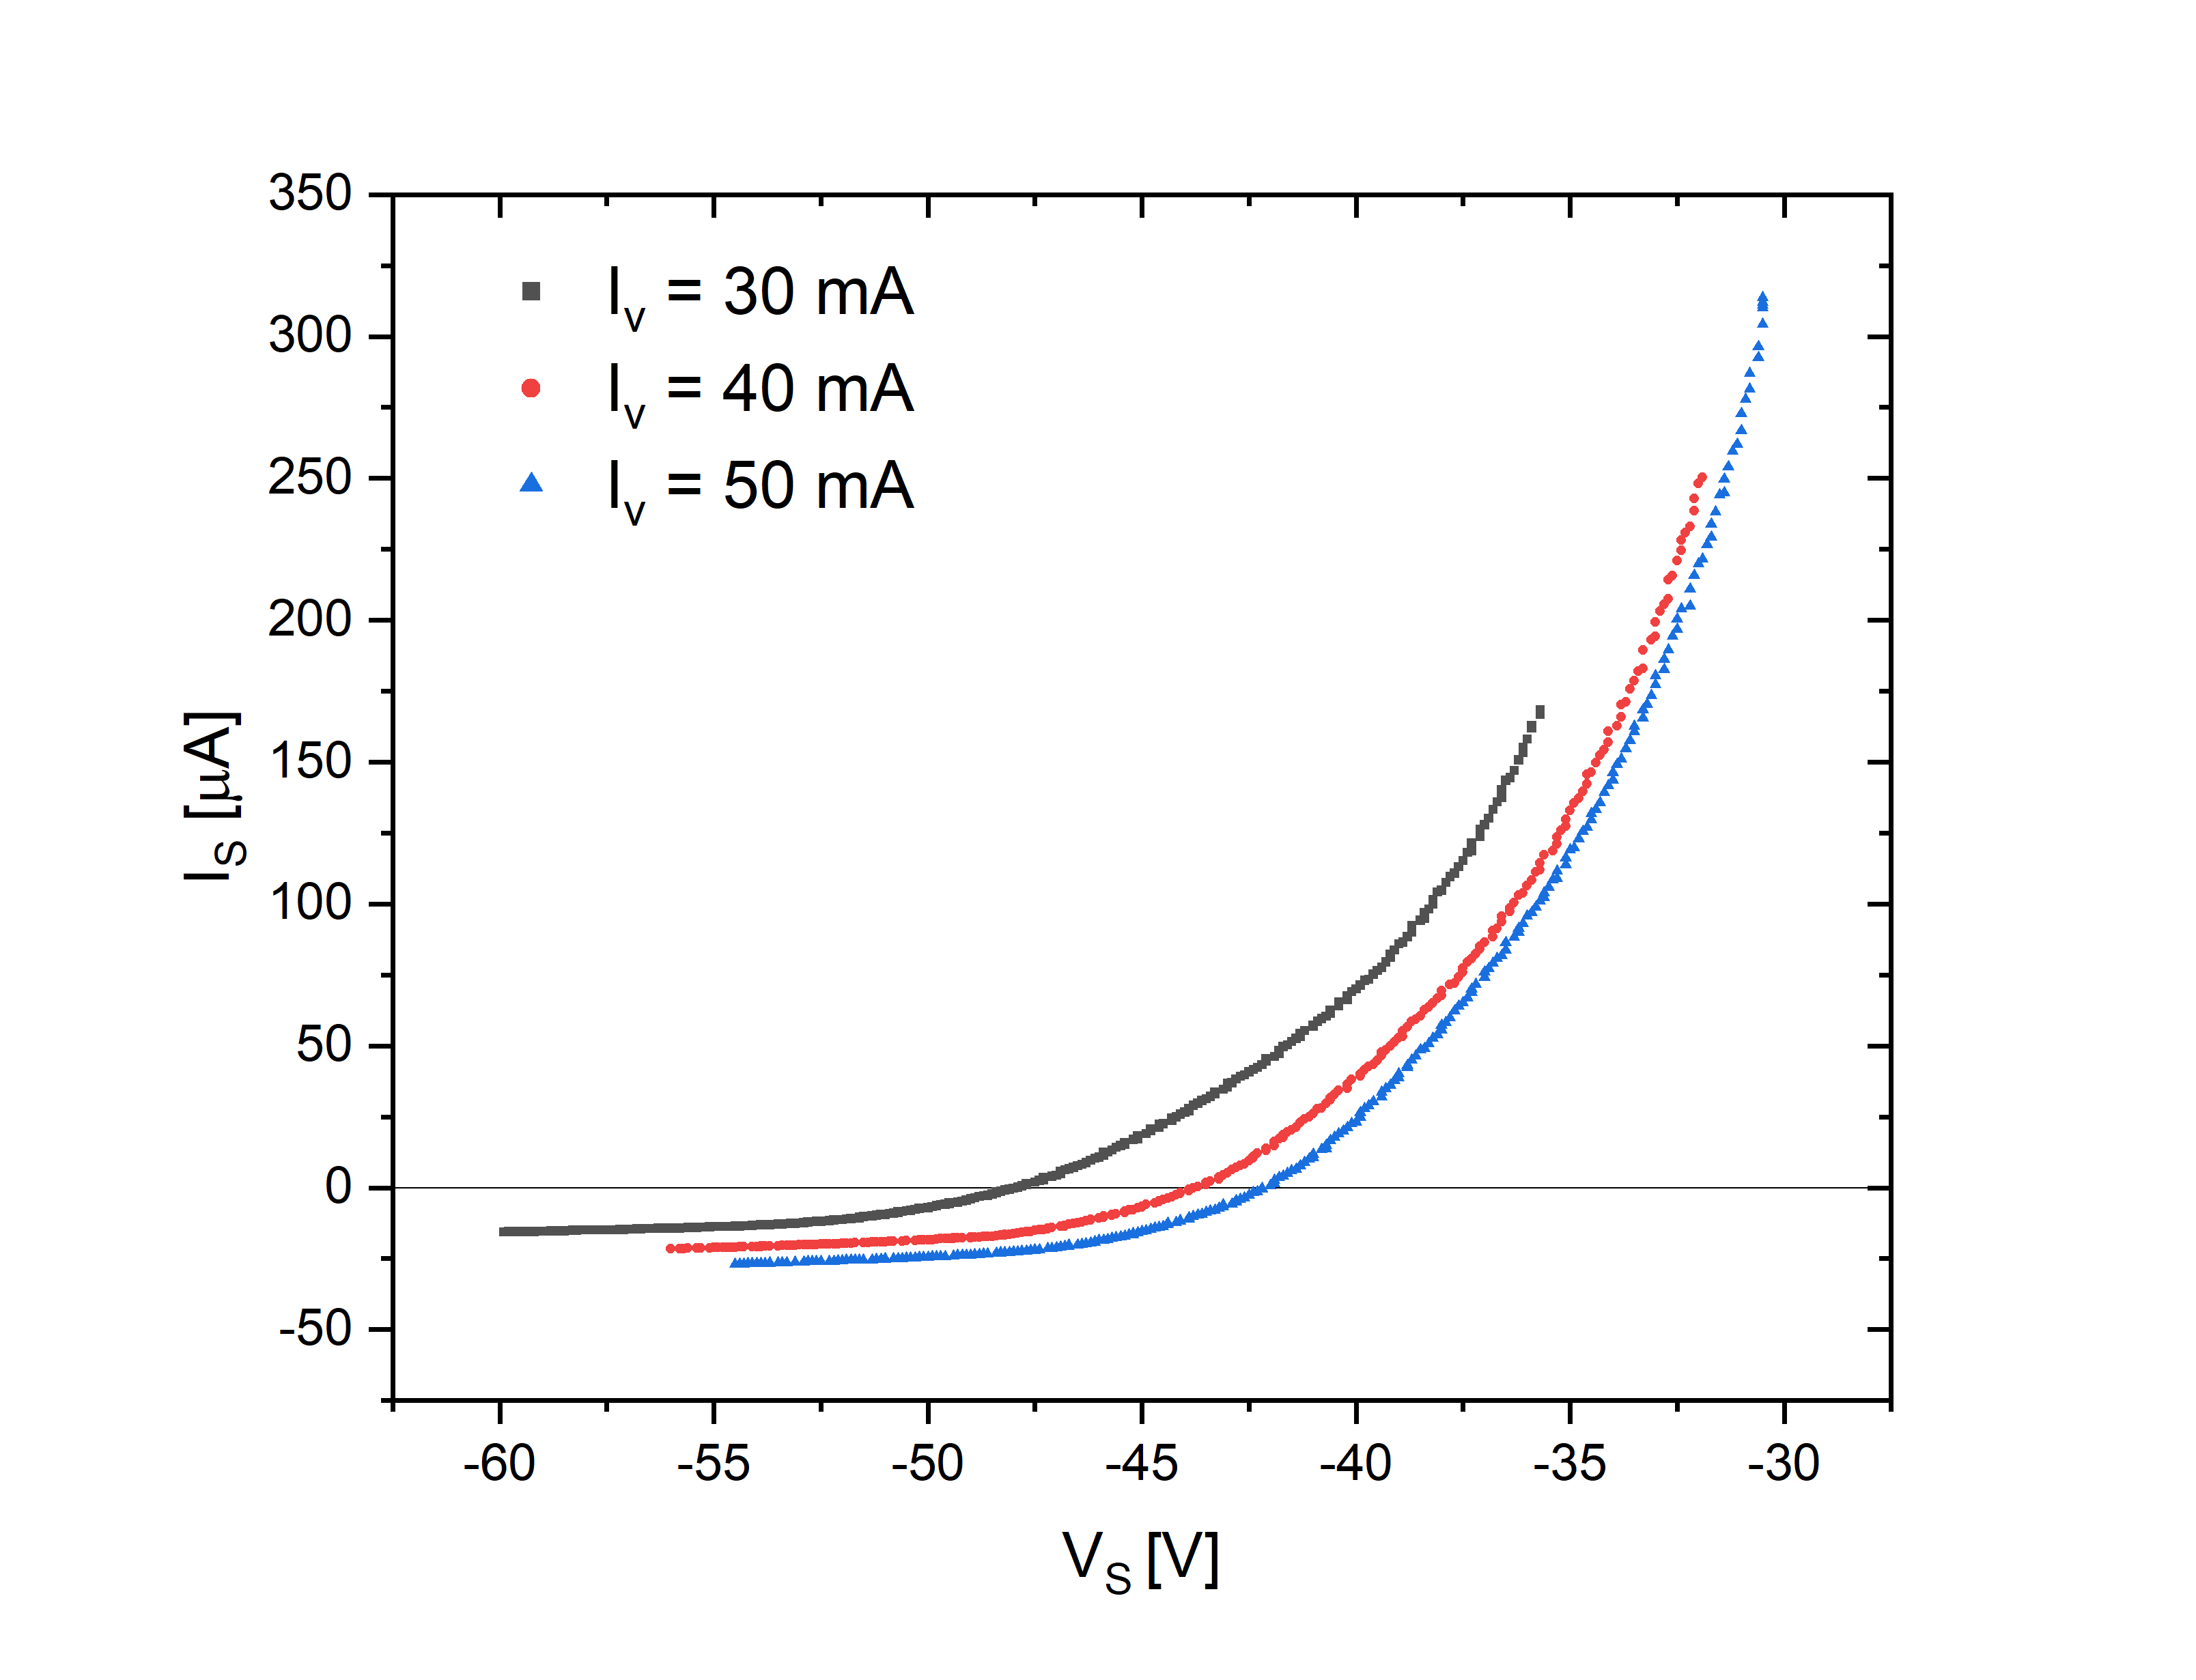
\includegraphics[width=145mm]{namerene012.png}
	\caption{Naměřené VA charakteristiky za konstantního tlaku 160 \si{\pascal}.}
	\label{namerene012}	
\end{figure}

\begin{figure}[h!]
	\centering
	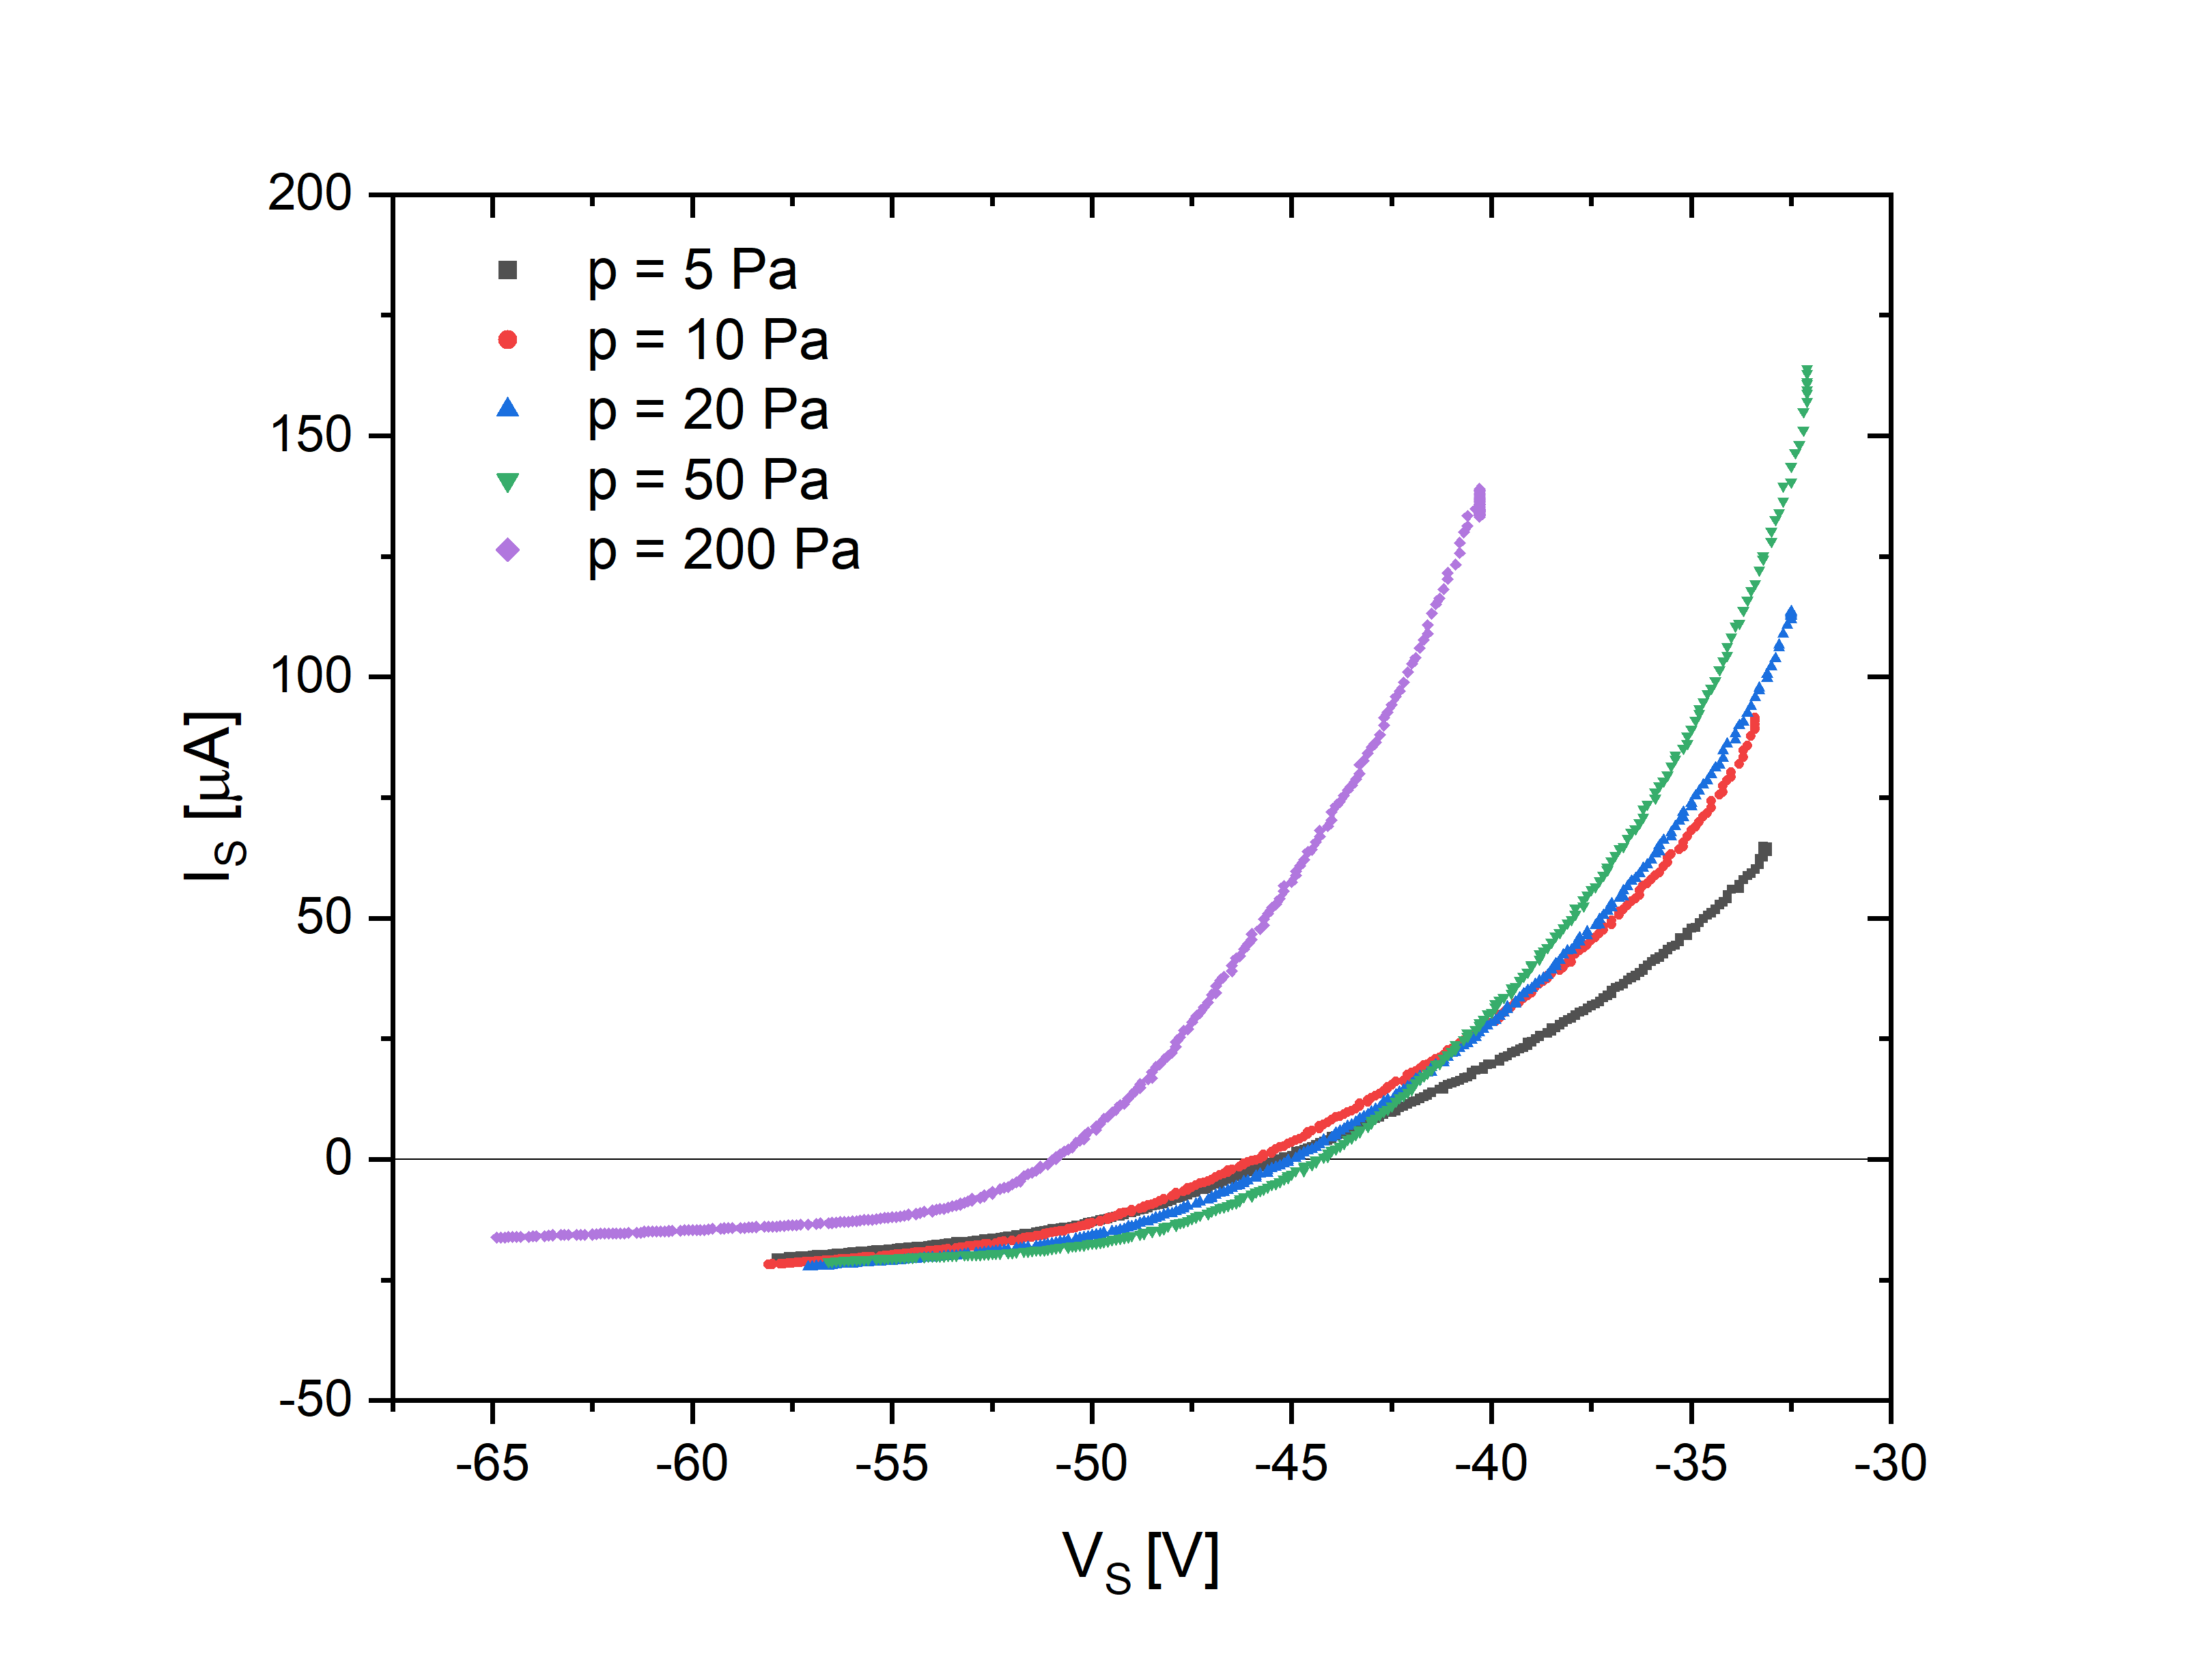
\includegraphics[width=145mm]{namerene34567.png}
	\caption{Naměřené VA charakteristiky za konstantního výbojového proudu 40 \si{\milli\ampere}.}
	\label{namerene34567}
\end{figure}

\newpage
Nyní je potřeba od charakteristik odečíst iontový proud, oblast, kde saturuje, 
jsme proložili 
přímkou. Názorné proložení pro VA
charakteristku za podmínek $p = 160$ \si{\pascal} a $I_\text{v}$ = 40 \si{\milli\ampere} je na obr. \ref{iiont}. Ve zbylých případech
jsme postupovali obdobně. VA charakteristiky s takto odečteným iontovým proudem jsou v grafech na obr. \ref{odectene012} a
\ref{odectene34567}.

\begin{figure}[h]
	\centering
	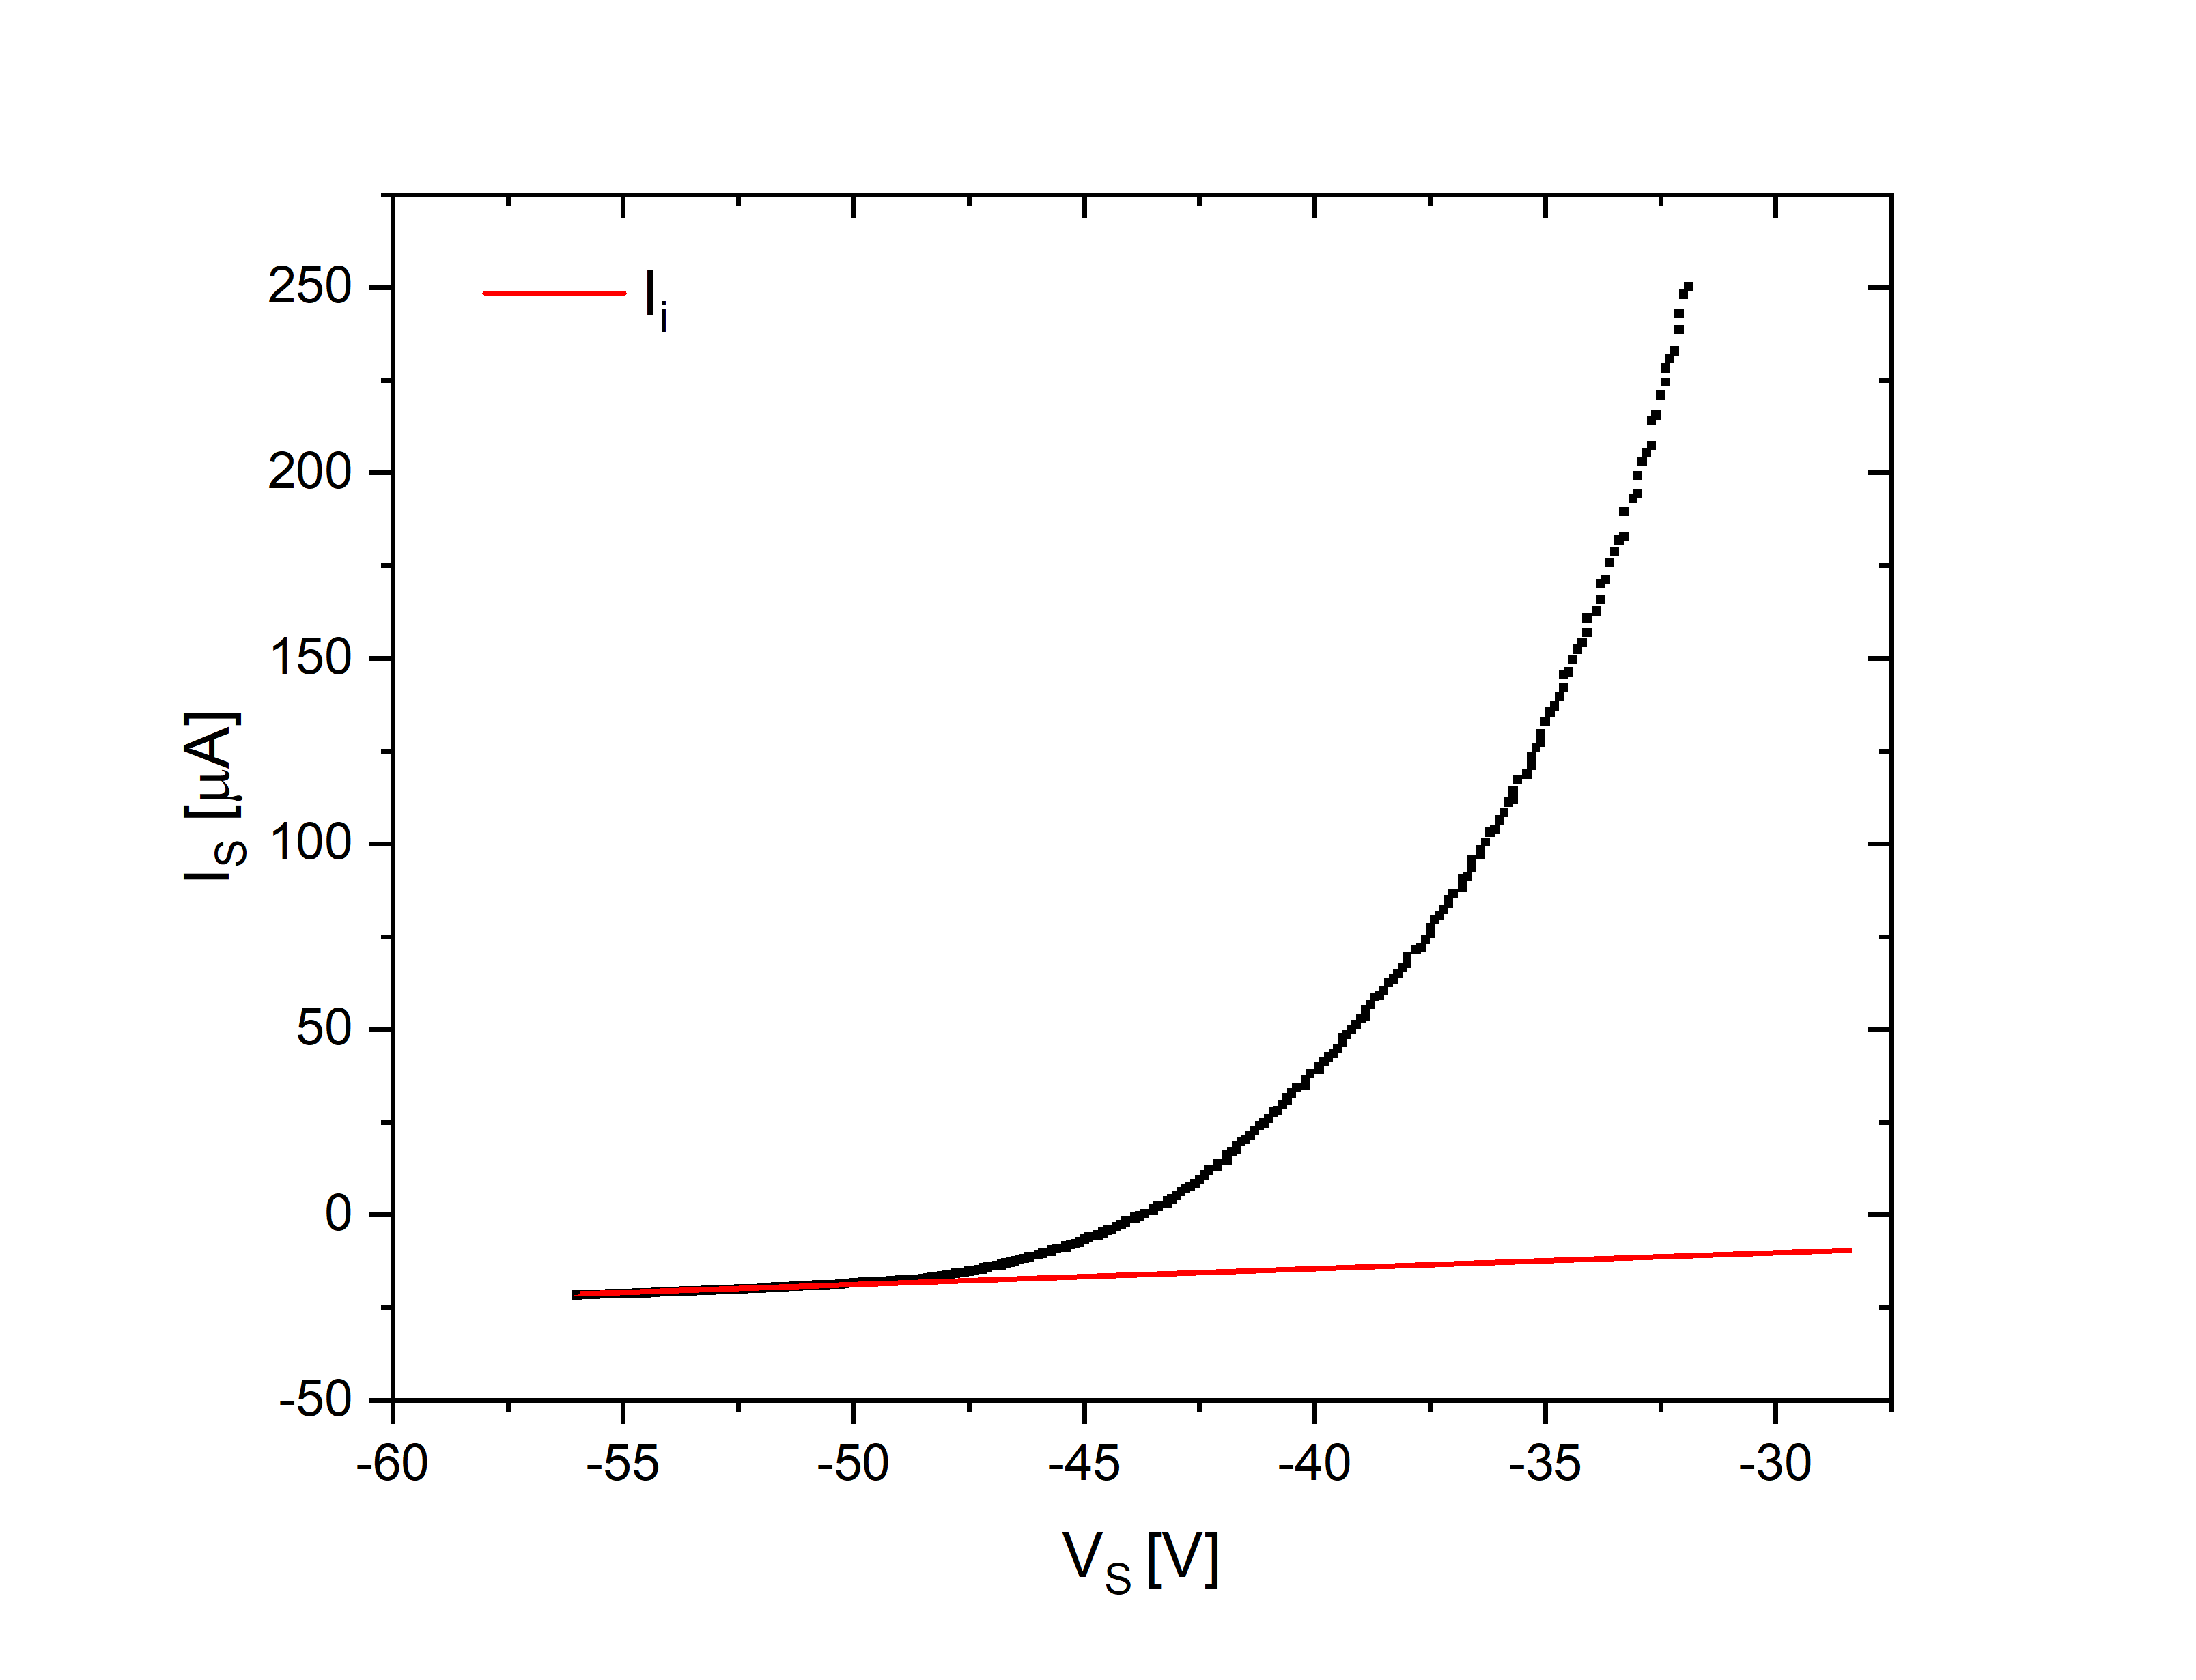
\includegraphics[width=145mm]{iiont.png}
	\caption{Rozdělení sondového proudu na iontový a elektronový pomocí 
	lineárního fitu saturovaného iontového proudu, $p = 160$ \si{\pascal} a 
	$I_\text{v} = 40$ \si{\milli\ampere}.}
	\label{iiont}
\end{figure}

\newpage
\begin{figure}[h!]
	\centering
	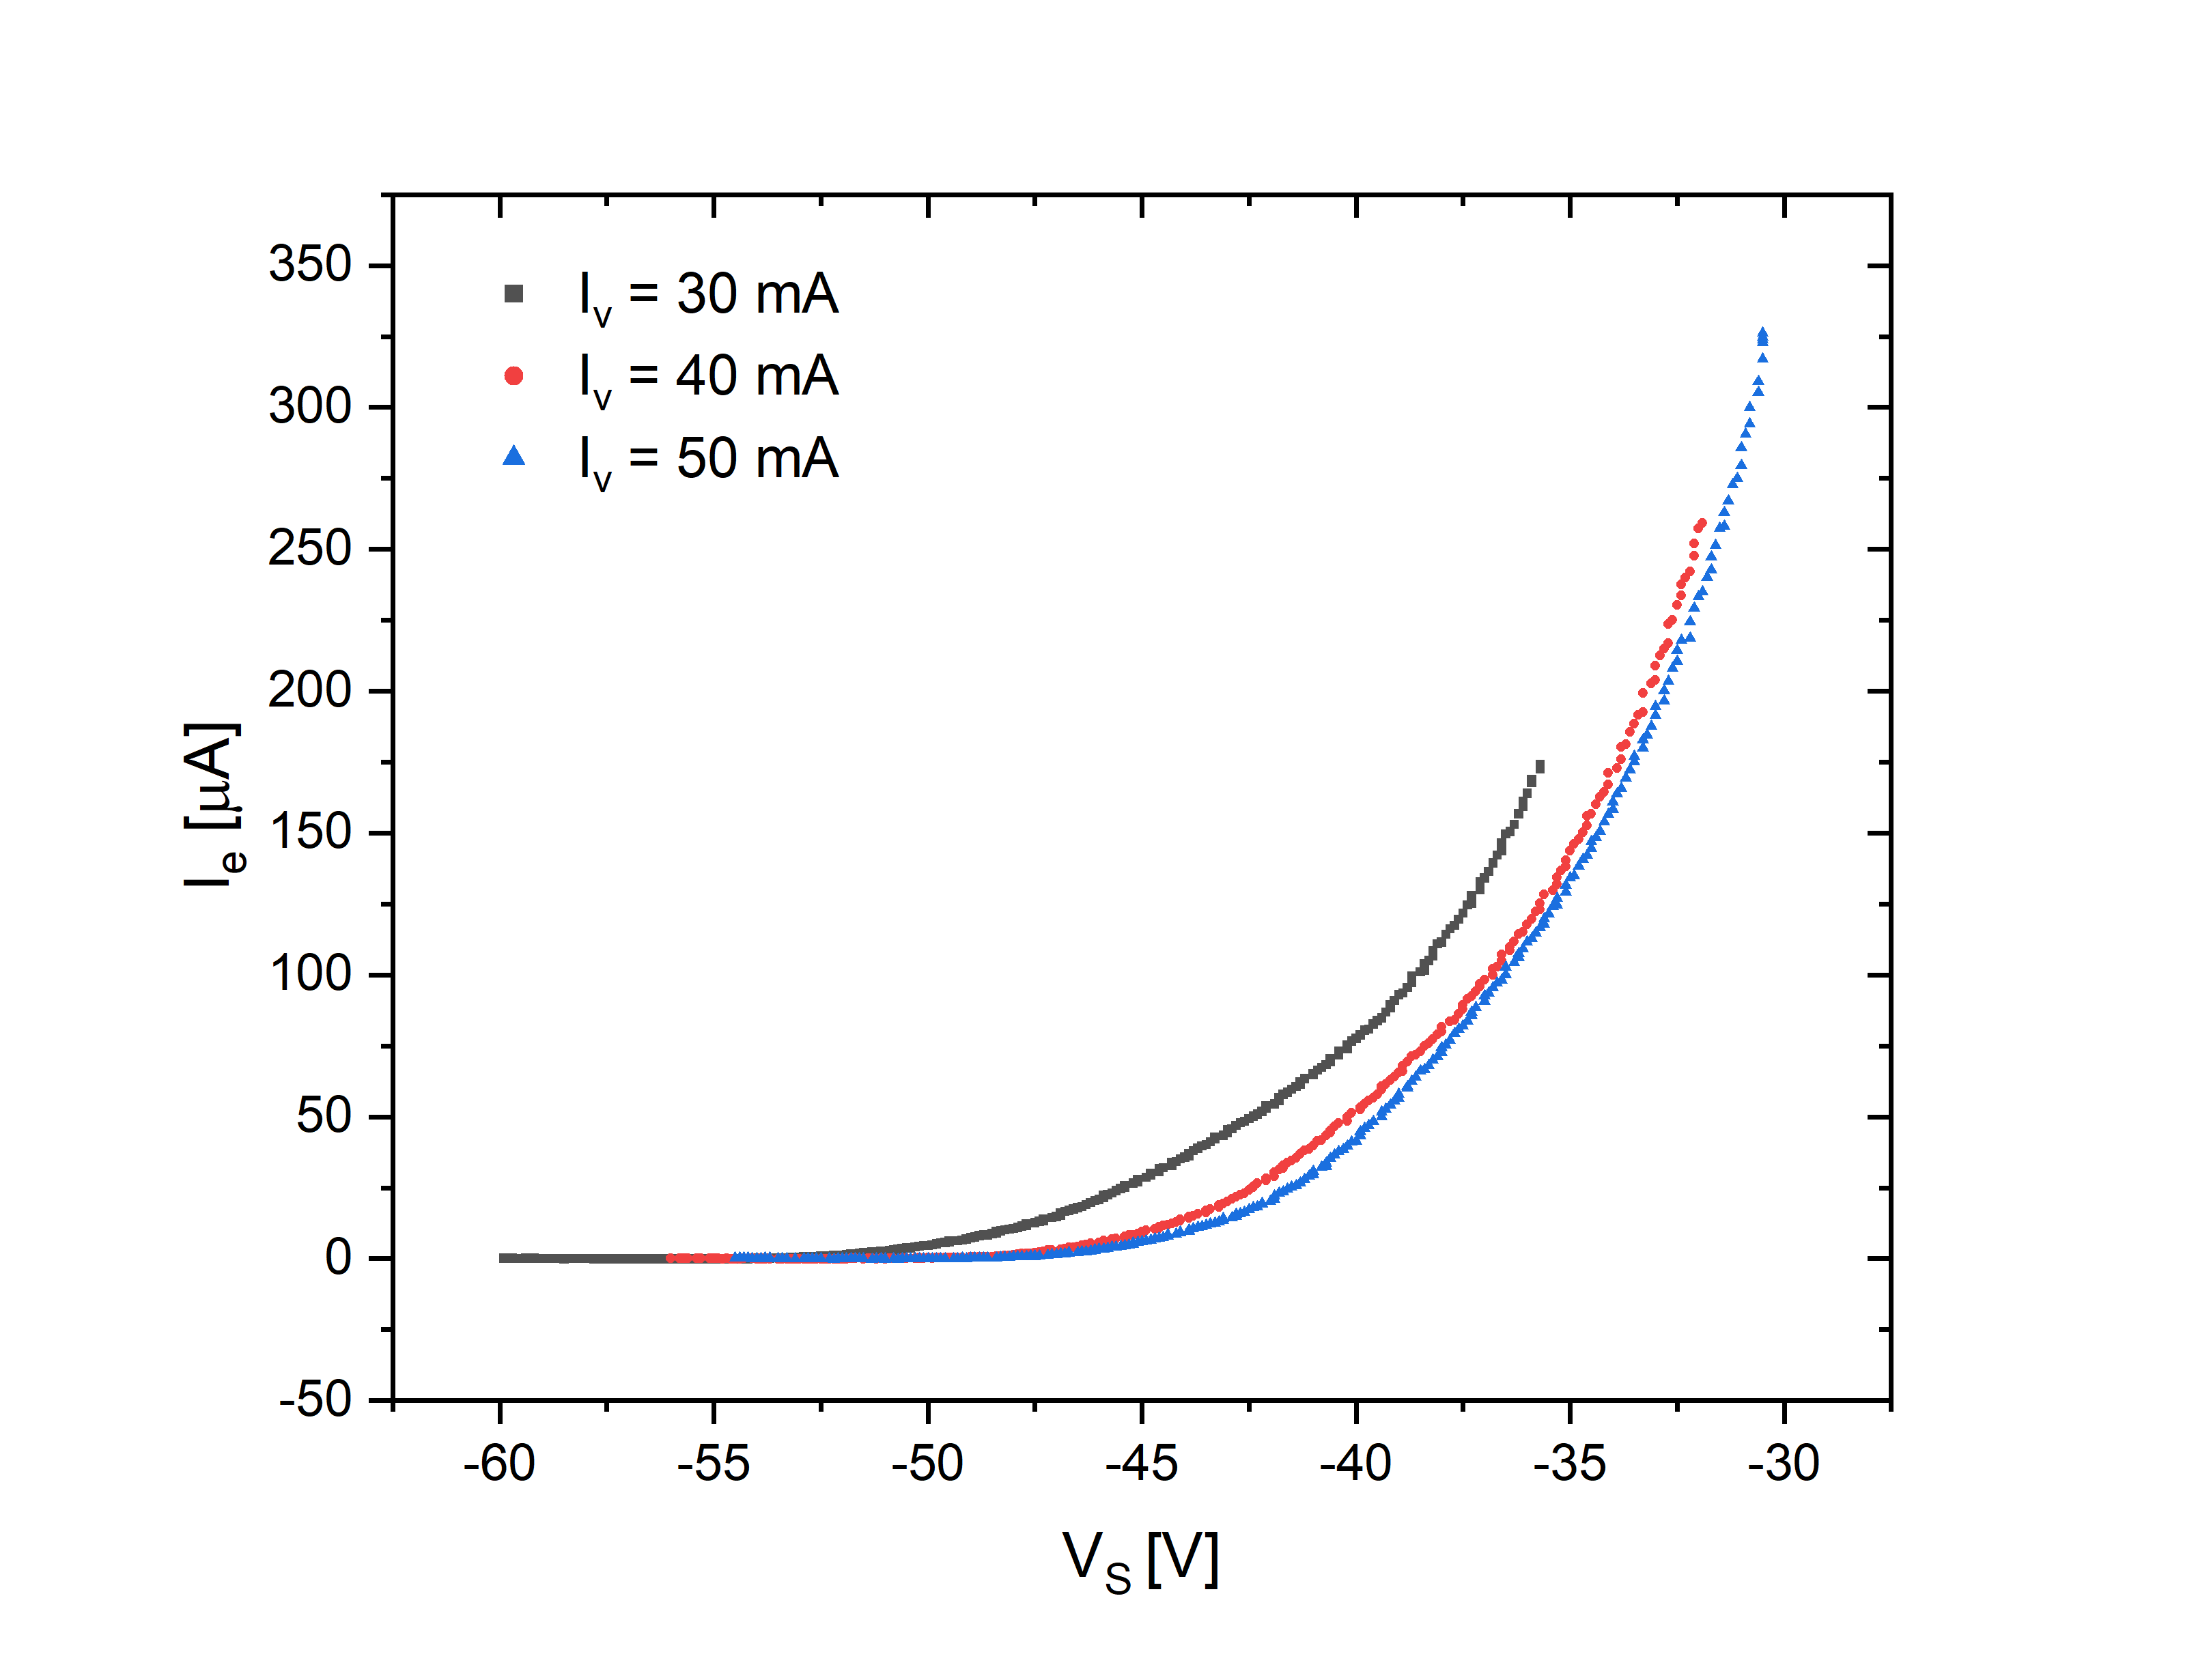
\includegraphics[width=135mm]{odectene012.png}
	\caption{VA charakteristiky s odečteným iontovým proudem pro měření s konstantním tlakem $p = 160$ \si{\pascal}.}
	\label{odectene012}
\end{figure}

\begin{figure}[h!]
	\centering
	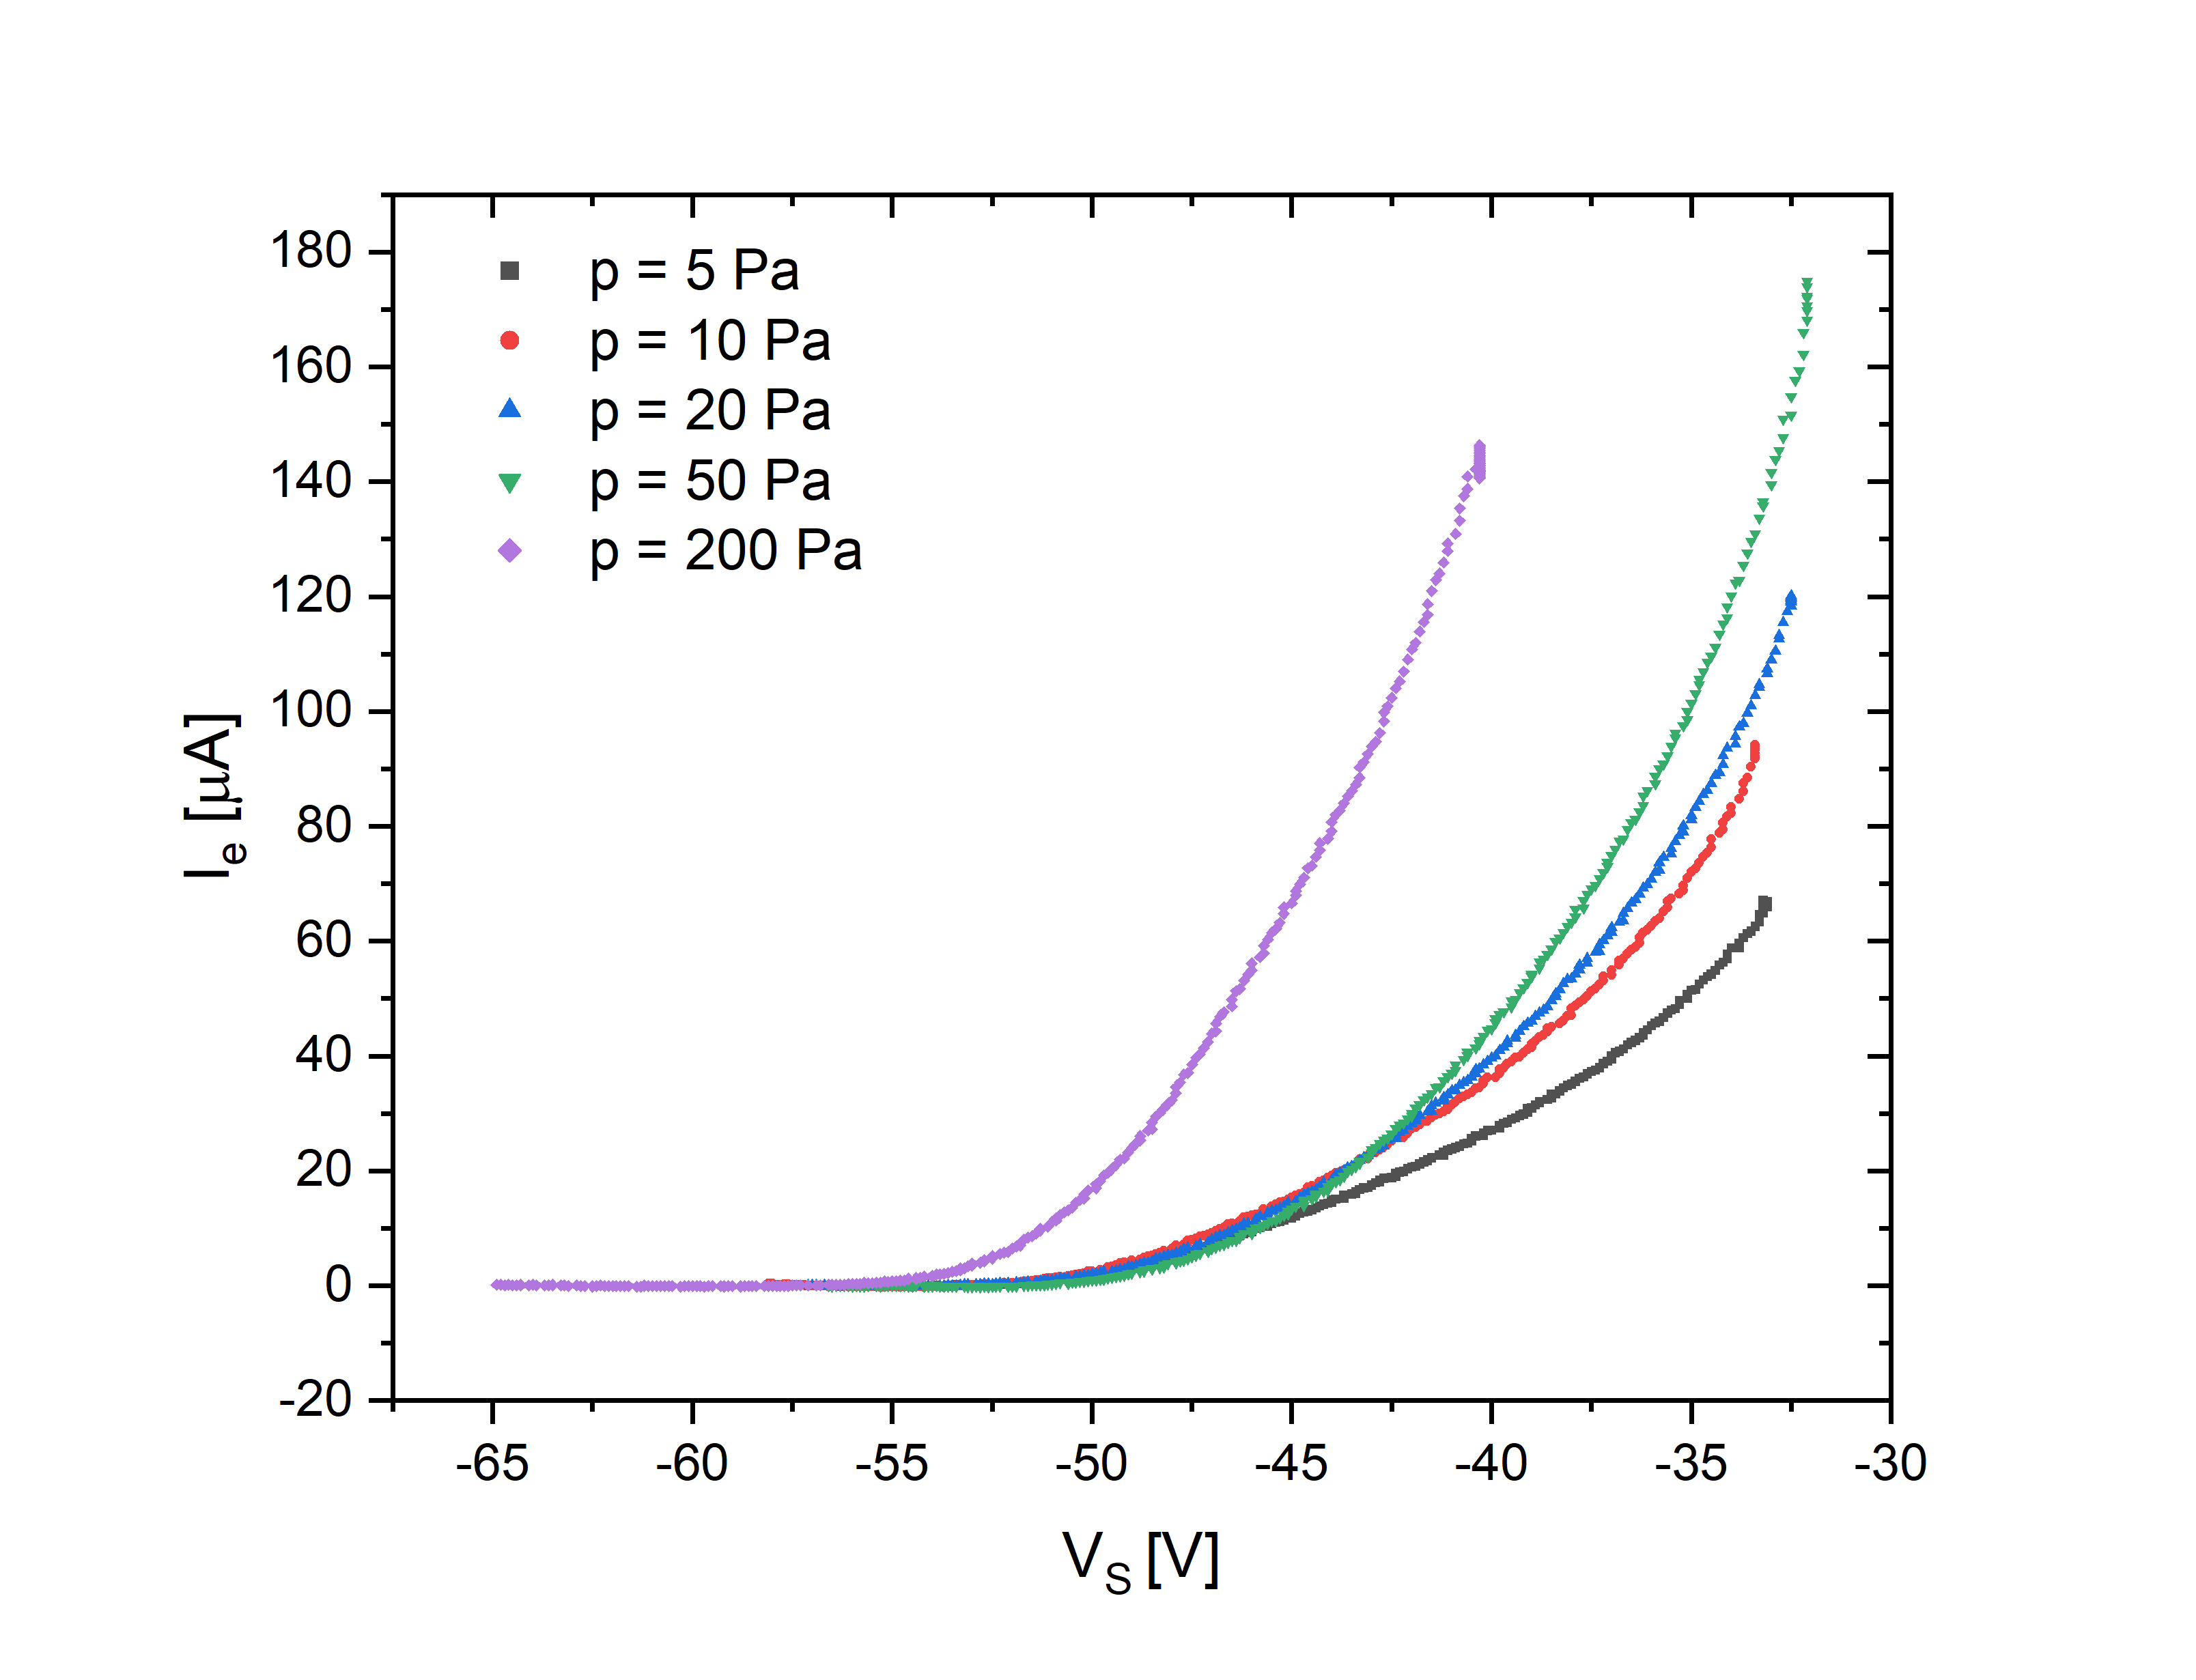
\includegraphics[width=135mm]{odectene34567.png}
	\caption{VA charakteristiky s odečteným iontovým proudem pro měření s konstantním proudem $I_\text{v} = 40$ \si{\milli\ampere}.}
	\label{odectene34567}
\end{figure}

\newpage
Potenciál plazmatu $V_\text{p}$ přibližně určíme ze zlomu VA charakteristik 
jako průsečík asymptot k lineárním částem zlogaritmovaných závislostí. Postup 
je vidět na obrázcích \ref{data1} až \ref{data7} vlevo a výsledné 
$V_\text{p}$~jsou uvedeny v tab. \ref{tab1}. Pokud máme proměřený dostatečný 
počet bodů, tak můžeme potenciál plazmatu určit také pomocí provedení druhé 
derivace, protože sondová charakteristika má v potenciálu plazmatu inflexní 
bod. Druhé derivace získané proložením dat polynomem 9. řádu
jsou vyneseny na obr.~\ref{data1sec} až \ref{data7sec}.
Nepodařilo se nám najít nulové body, spokojili jsme se vždy
s lokálním minimem.
Takto určený potenciál plazmatu je v tab.~\ref{tab1} označen jako 
$V_\text{p,d}$. Vždy platí, že~$V_\text{p}$ je větší než $V_\text{fl}$. Stejně 
jako 
$V_\text{fl}$, potenciál plazmatu s~rostoucím výbojovým proudem roste, při změně
tlaku nevykazuje žádný trend. Nyní můžeme ze vztahu \eqref{Usondy} dopočítat $U_\text{S}$. Pokud následně vyneseme do grafů závislosti $\ln
I_{\text{e}}$~=~$-\frac{e}{kT_e}U_\text{S}+C$~pro oblasti $-2(V_\text{p} - 
V_\text{{fl}}) \leq U_\text{S} \leq 0$, můžeme z
elektronového proudu pro $U_\text{S} = 0$ dle vztahu \eqref{eproud} dopočítat koncentraci elektronů. Závislosti $\ln I_{\text{e}} =
f(U_\text{S})$ proložené přímkou jsou na obr. \ref{data1} až 
\ref{data7sec} vpravo. Výsledné elektronové teploty a koncentrace
elektronů jsou v tab. \ref{tab2}, index~d značí hodnoty získané
z druhé derivace. S rostoucím výbojovým proudem roste i 
koncentrace elektronů. Metodou průsečíků asymptot teplota elektronů s výbojovým 
proudem klesá, ale metodou druhé derivace je konstantní. S rostoucím
tlakem pozorujeme klesající teplotu a~rostoucí koncentrace elektronů při 
použití obou metod. Rozdílem výsledků metod je hlavně nižší plazmový potenciál 
a koncentrace elektronů, jejichž závislost je výraznější při použití metody 
druhé derivace. V obou metodách jsme však ve stejném řádu 
$10^{14}$\,\si{\per\cubic\meter}.

\begin{center}
	\begin{table}[h!]
		\centering
		\caption{Plovoucí a plazmové potenciály}
		\label{tab1}
		\begin{tabular}{|c|c|c|c|c|c|c|c|} \hline
			\multicolumn{4}{|c|}{$p$ = 160 \si{\pascal}}& 
			\multicolumn{4}{c|}{$I_\text{v}$ = 40 \si{\milli\ampere} }  \\ 
			\hline
			$I_\text{v}$ [\si{\milli\ampere}] &  $V_\text{fl}$ [V] & 
			$V_\text{p}$ [V] & $V_\text{p,d}$ [V] & $p$ [\si{\pascal}] &  
			$V_\text{fl}$ [V] & $V_\text{p}$ [V] & $V_\text{p,d}$ \\ \hline
			30 & -48,0 & -47,7 & -43,4 & 8 & -45,3 & -44,8 & -43,8 \\ \hline
			40 & -43,8 & -43,4 & -39,7 & 16 & -45,8 & -45,2 & -44,4 \\ \hline
			50 & -42,2 & -41,6 & -37,5 & 32 & -45,0 & -44,6 & -43,4 \\ \hline
			& & & & 80 & -44,4 & -43,9 & -42,8 \\ \hline
			& & & & 320 & -50,9 & -49,9 & -45,8 \\ \hline
			
		\end{tabular}
	\end{table}
\end{center}


\begin{center}
	\begin{table}[h!]
		\centering
		\caption{Teploty a koncentrace elektronů}
		\label{tab2}
		\begin{tabular}{|c|c|c|c|c|c|} \hline
			 \multicolumn{3}{|c|}{$p$ = 160 \si{\pascal}}& \multicolumn{3}{c|}{$I_\text{v}$ = 40 \si{\milli\ampere} }  \\ \hline
			$I_\text{v}$ [\si{\milli\ampere}] &  $T$ [eV] & $n_\text{e} [10^{14}\si{\per\meter\cubed}$] & $p$ [\si{\pascal}] &  $T$ [eV] & $n_\text{e} [10^{14}\si{\per\meter\cubed}]$ \\ \hline
			30 & 3,3 & 1,0 & 8 & 4,6 & 0,8\\ \hline
			40 & 2,8 & 1,6 & 16 & 4,3 & 1,1 \\ \hline
			50 & 2,6 & 2,3 & 32 & 4,0 & 1,2\\ \hline
			&  &  & 80 & 3,7 & 1,4 \\ \hline
			& &  & 320 & 2,2 & 1,7 \\ \hline
			$I_\text{v}$ [\si{\milli\ampere}] &  $T_\text{d}$ [eV] & 
			$n_\text{e,d} [10^{14}\si{\per\meter\cubed}$] & $p$ [\si{\pascal}] 
			&  $T_\text{d}$ [eV] & $n_\text{e,d} 
			[10^{14}\si{\per\meter\cubed}]$ \\ \hline
			30 & 2,4 & 4,0 & 8 & 4,4 & 1,1\\ \hline
			40 & 2,4 & 5,4 & 16 & 4,0 & 1,3 \\ \hline
			50 & 2,5 & 7,7 & 32 & 3,8 & 1,6\\ \hline
			&  &  & 80 & 3,5 & 2,0 \\ \hline
			& &  & 320 & 2,0 & 6,0 \\ \hline
			
		\end{tabular}
	\end{table}
\end{center}
\newpage
\begin{figure}[h]
	\centering
	\begin{subfigure}[b]{.49\textwidth}
		\centering
		\scalebox{.34}{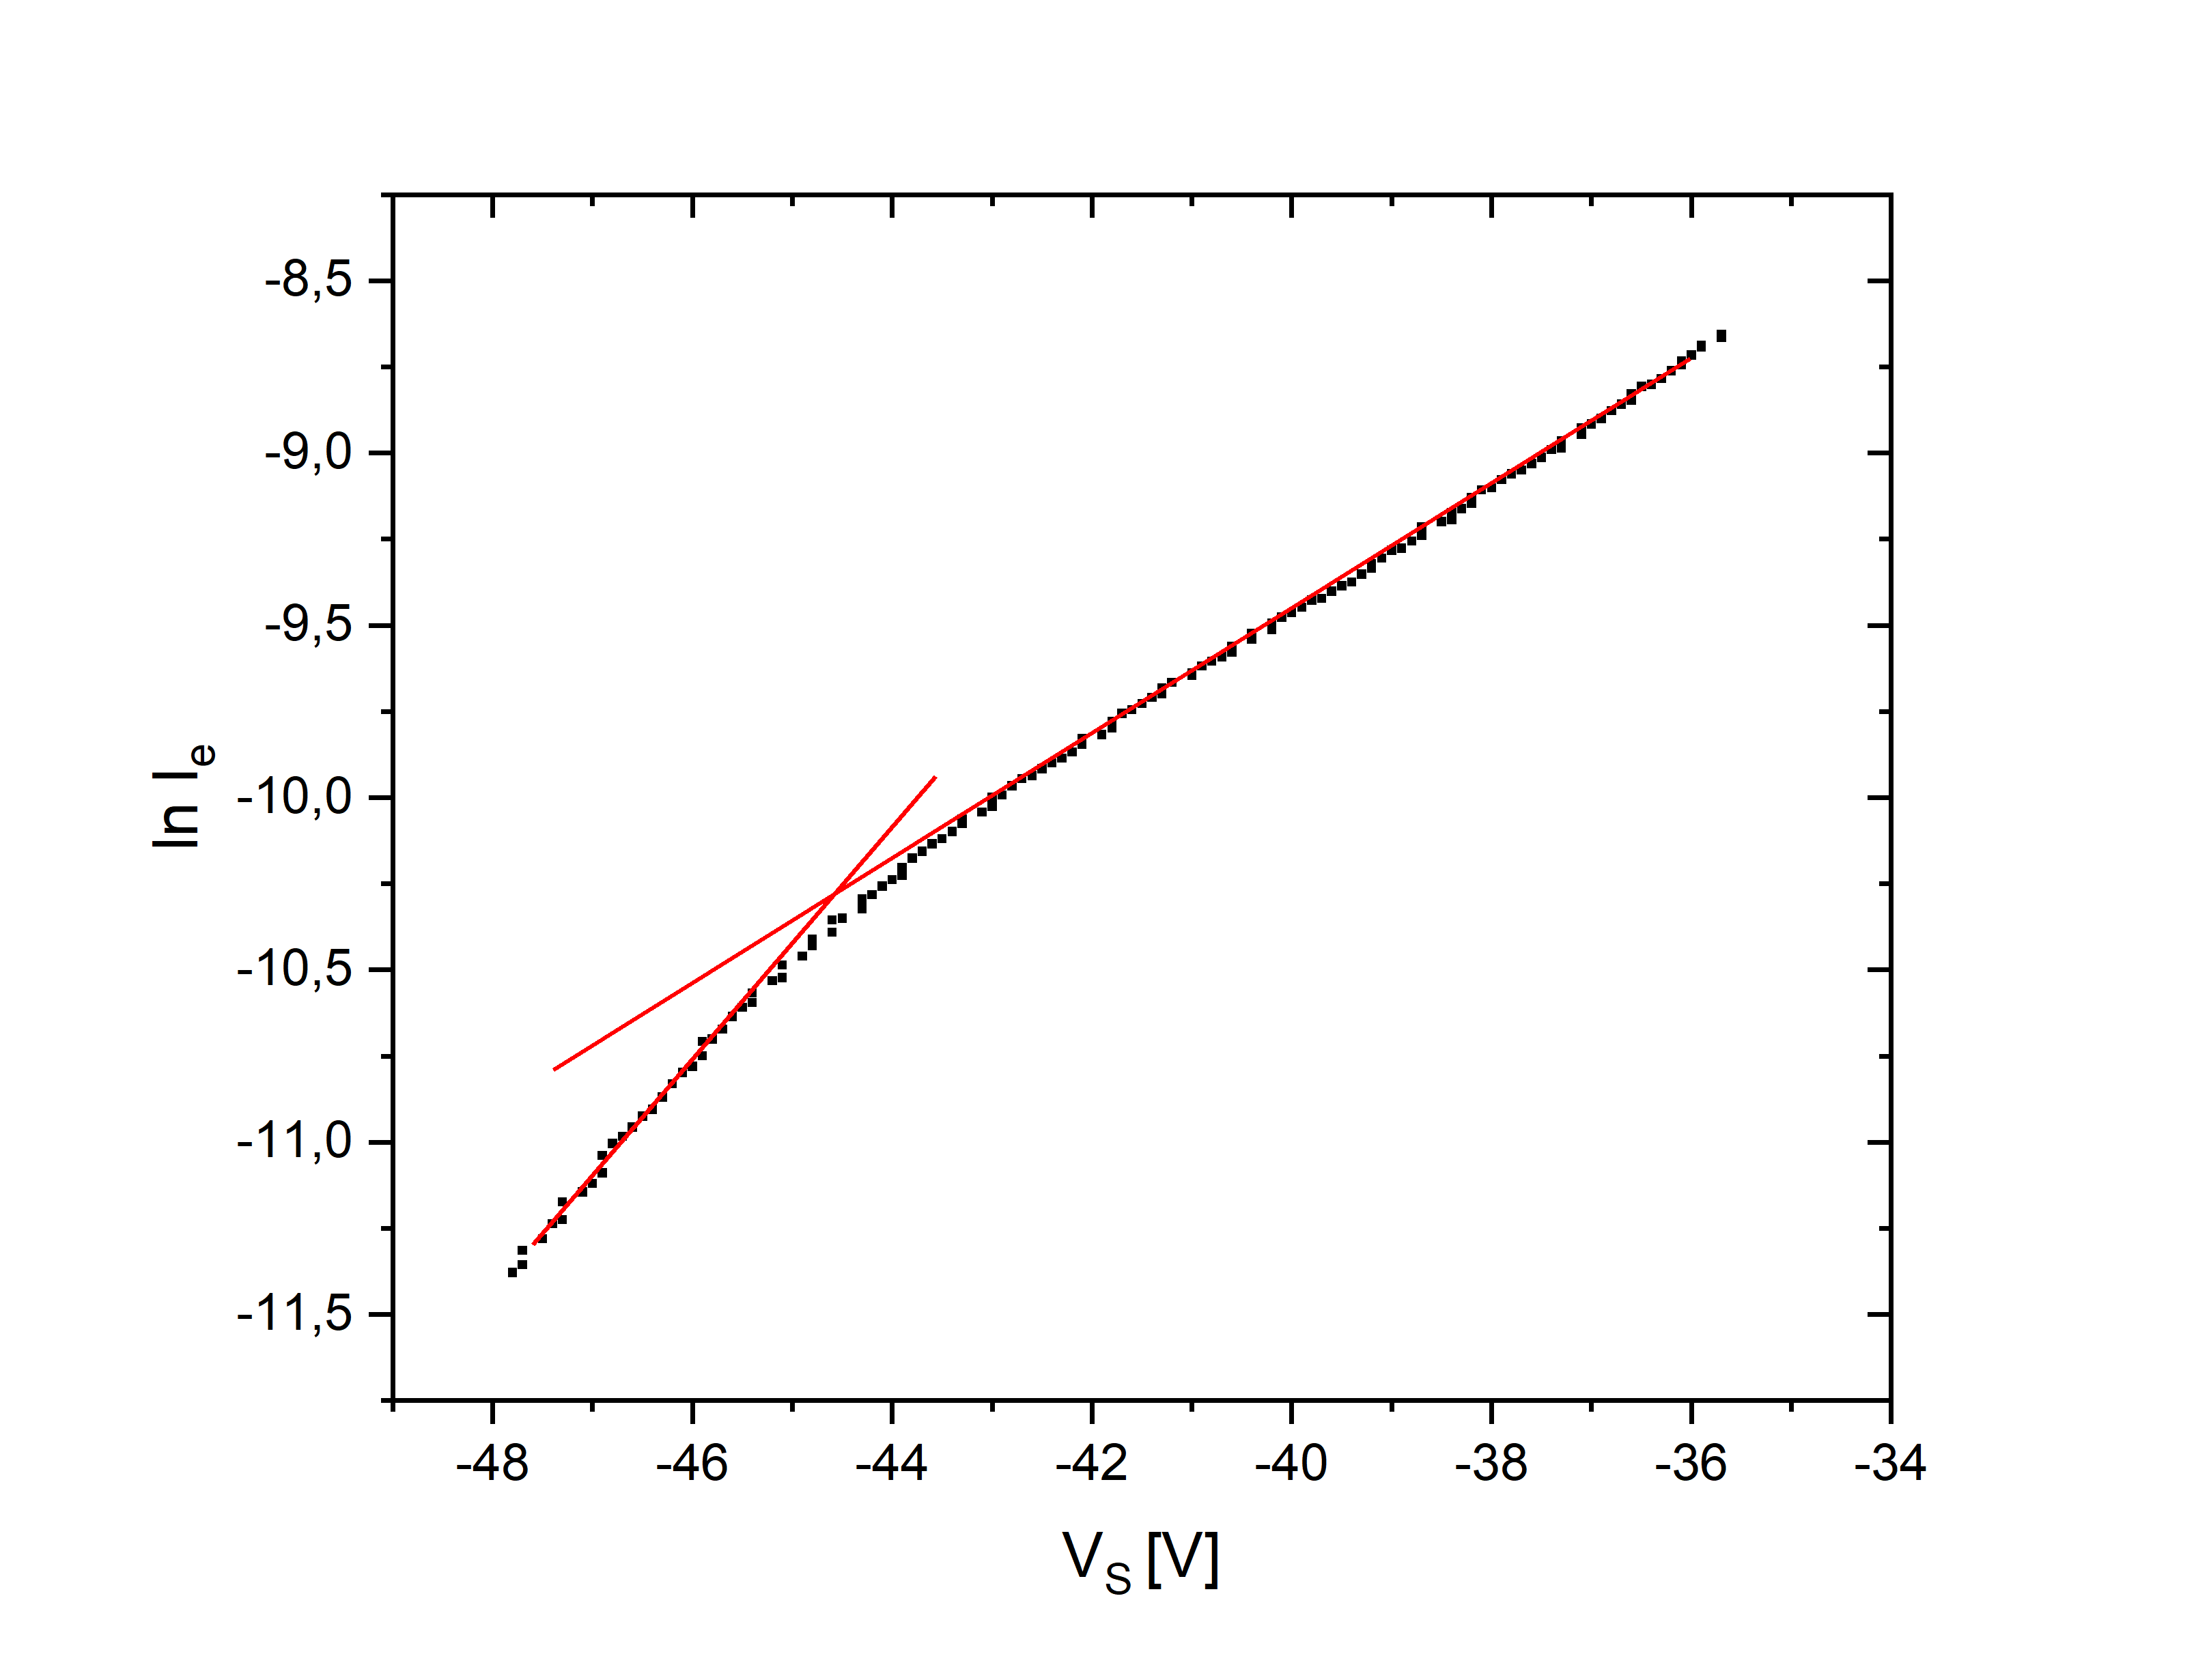
\includegraphics{data1Vp.png}}
		%\caption{$f(t) = 1/n$}
	\end{subfigure}
	\begin{subfigure}[b]{.49\textwidth}
		\centering
		\scalebox{.34}{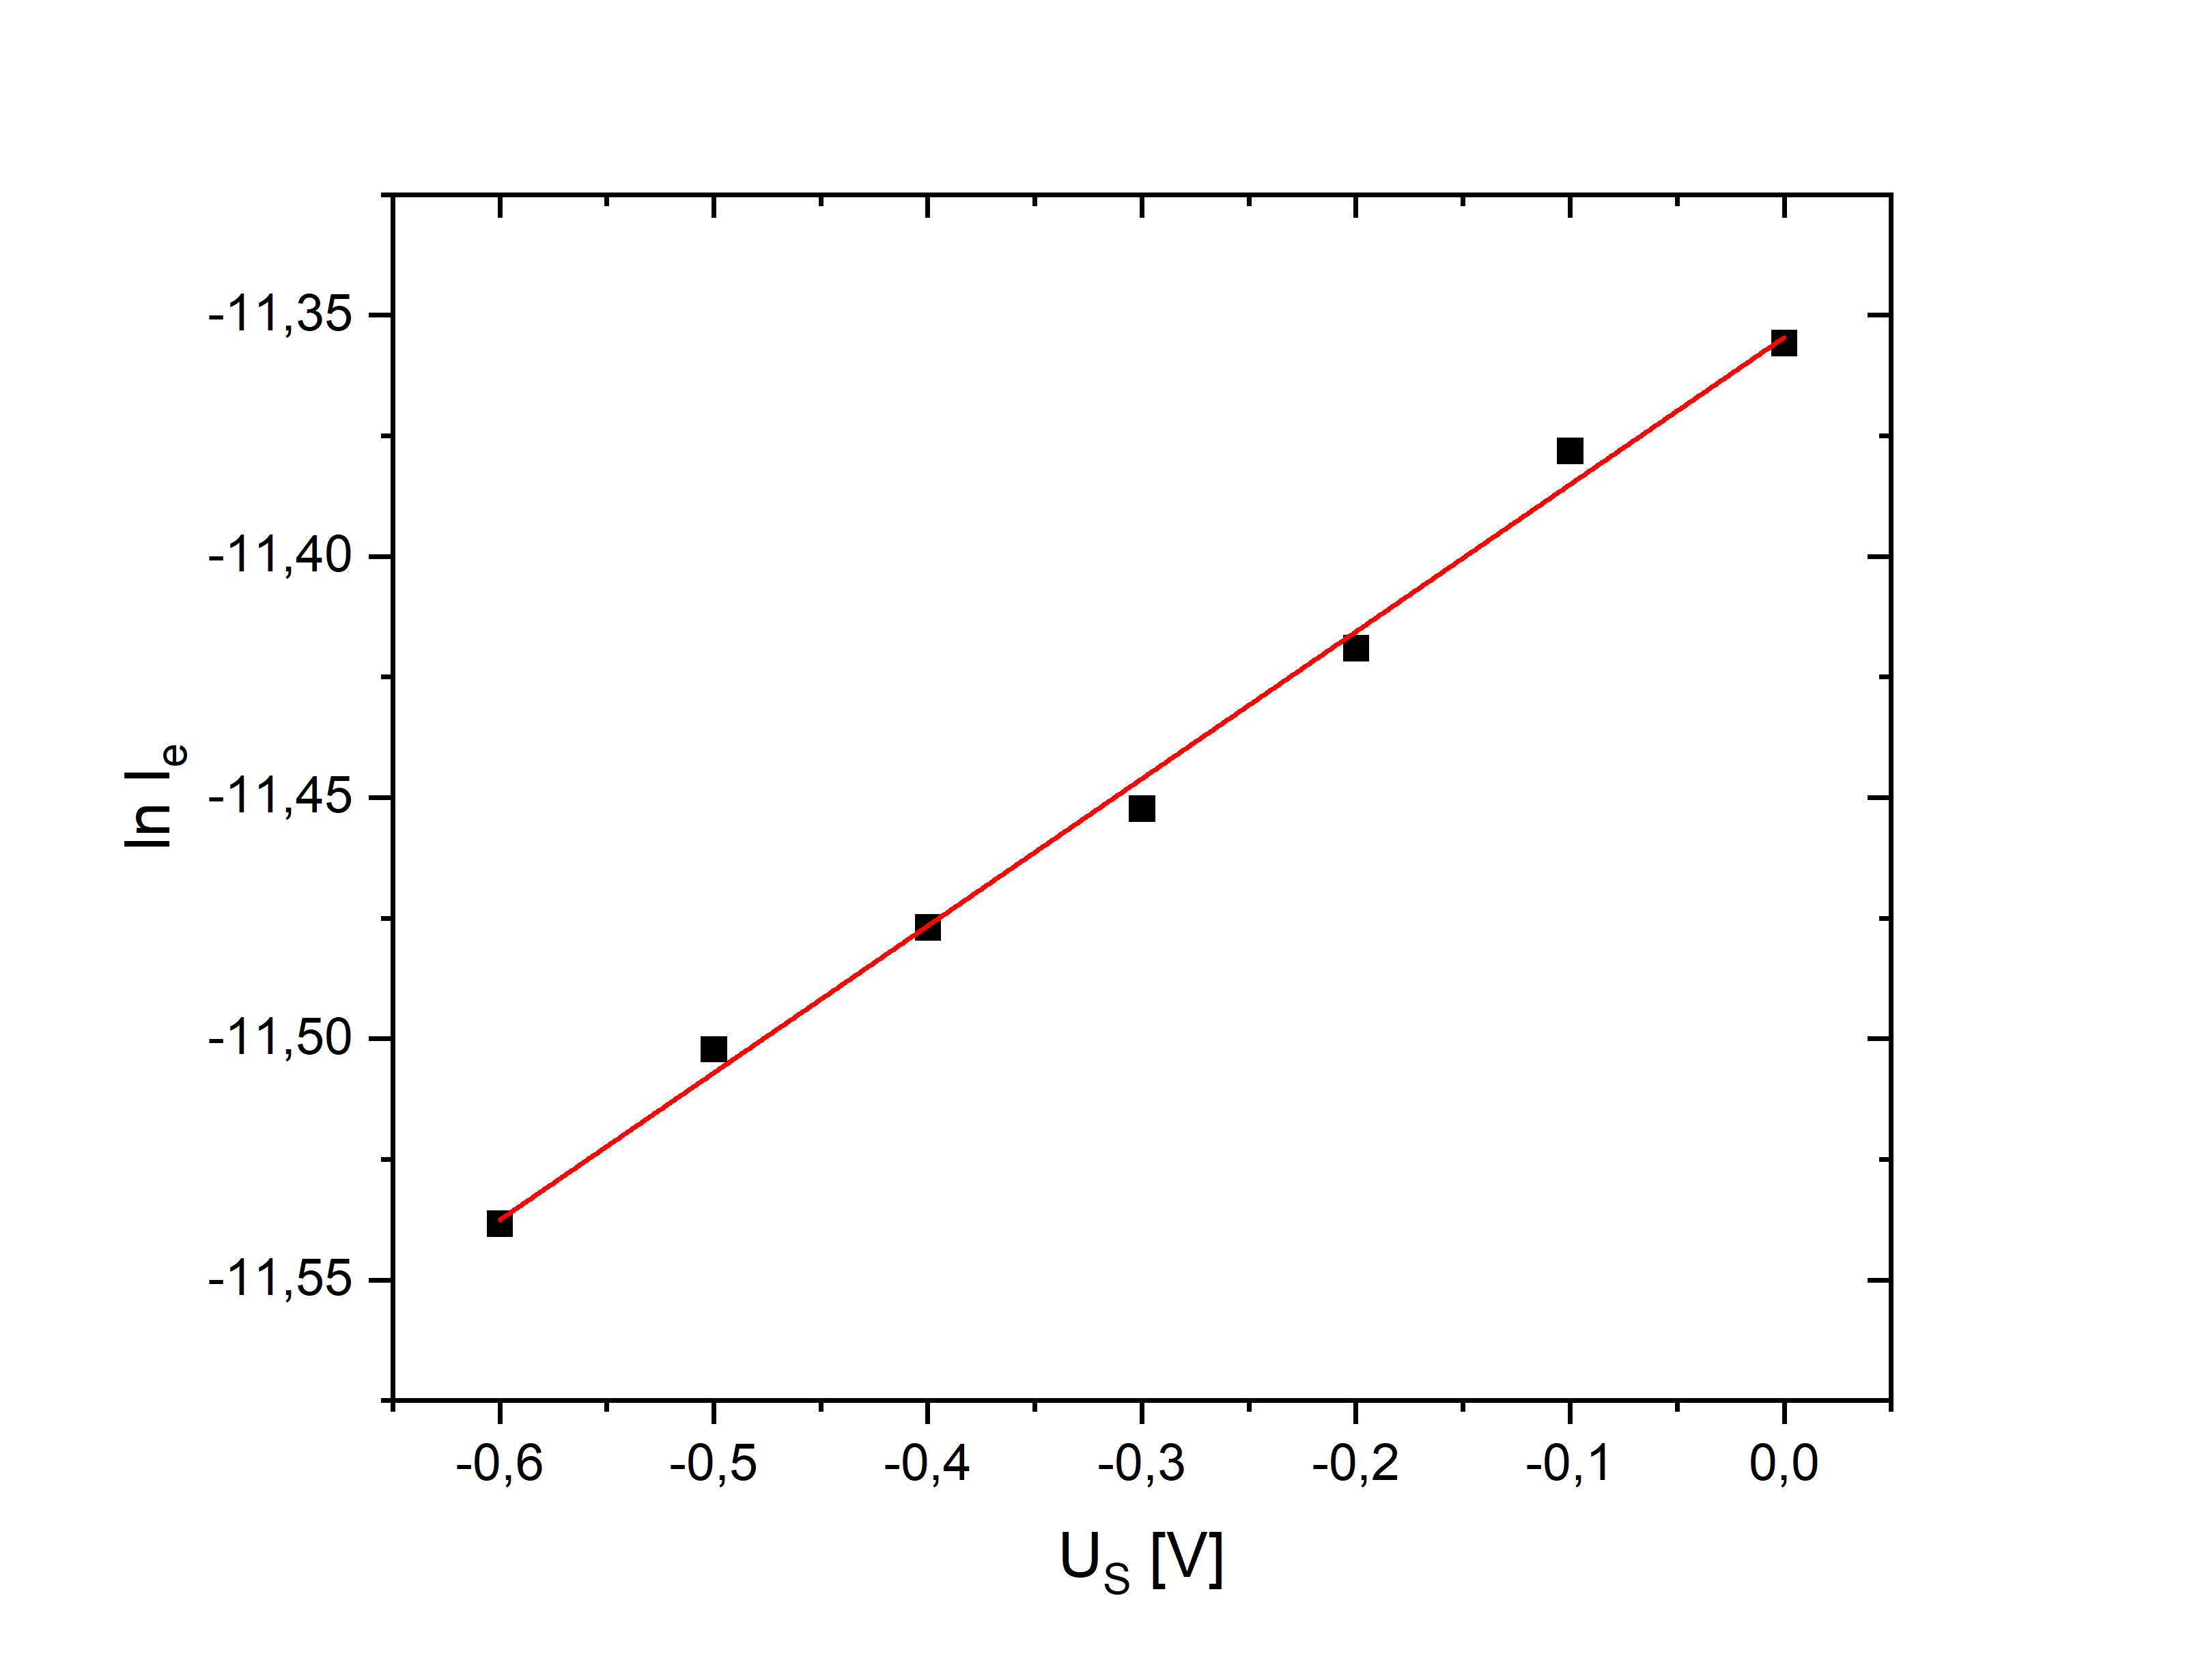
\includegraphics{data1T.png}}
		%\caption{$f(t) = \ln n$}
	\end{subfigure}
	\caption{Stanovení potenciálu plazmatu a elektronové teploty pomocí 
	průsečíku asymptot, $p = 160$ \si{\pascal} a $I_\text{v} = 30$ 
	\si{\milli\ampere}.}
	\label{data1}
\end{figure}

\begin{figure}[h]
	\centering
	\begin{subfigure}[b]{.49\textwidth}
		\centering
		\scalebox{.34}{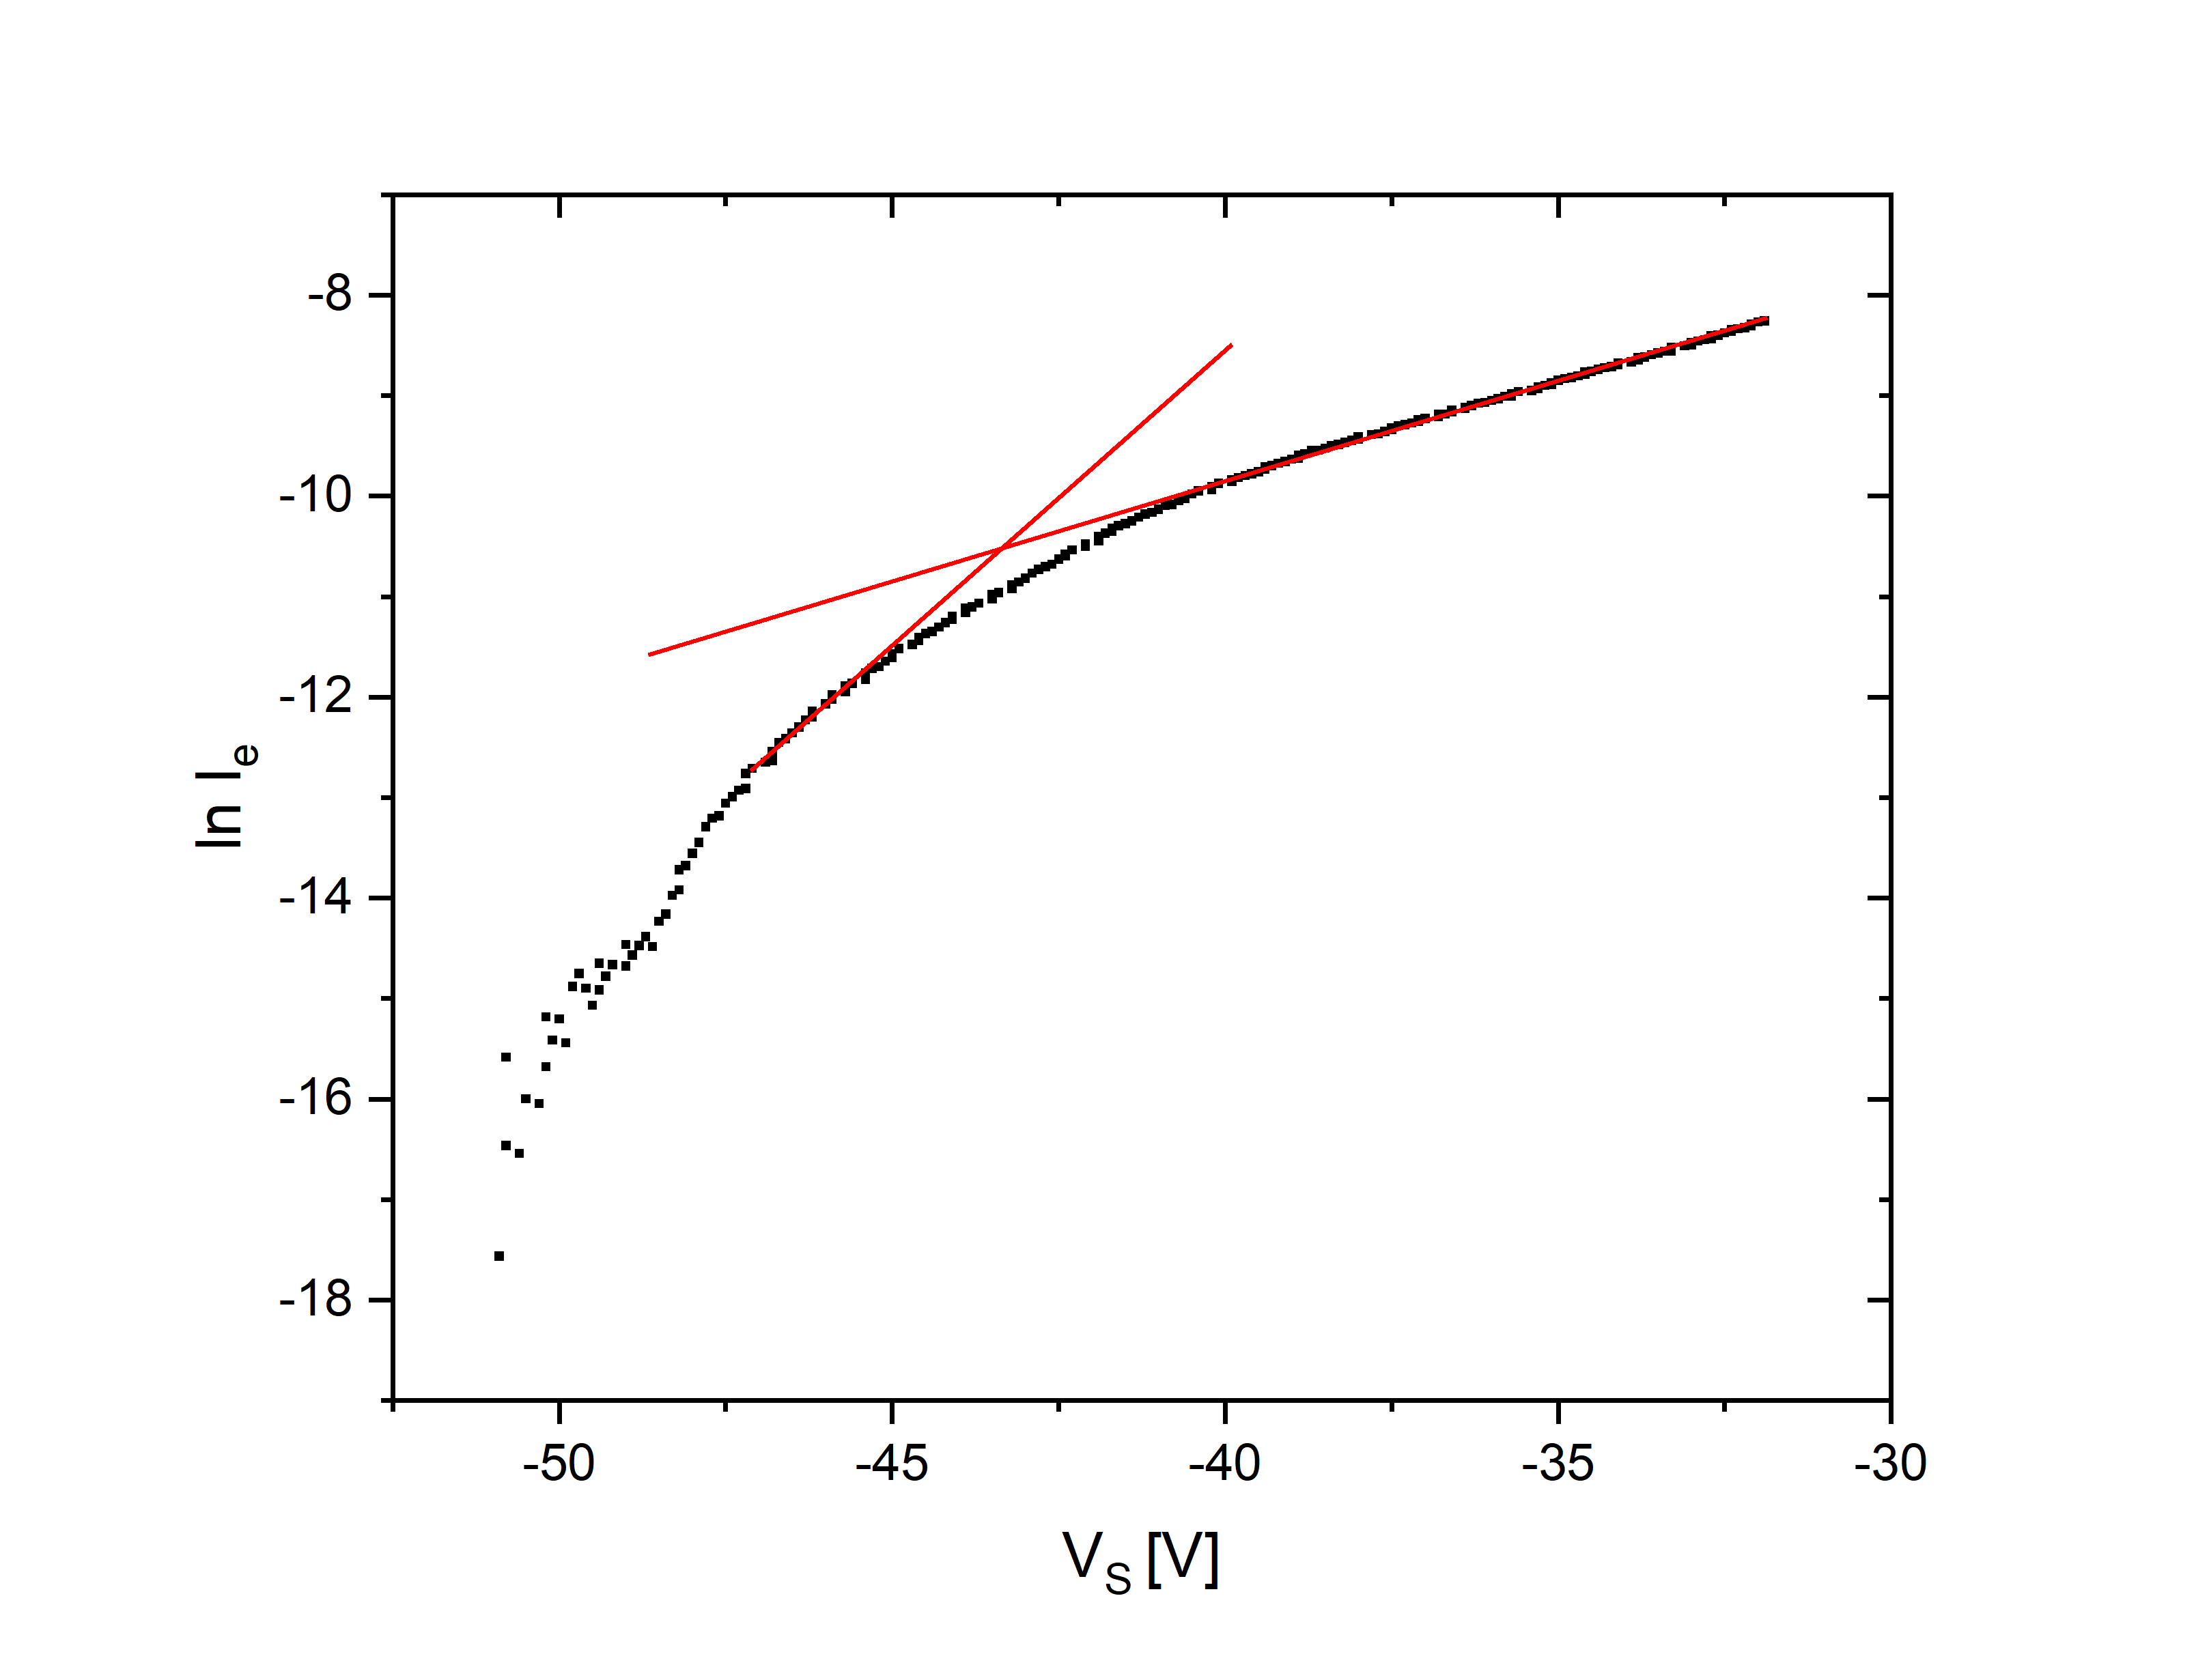
\includegraphics{data0Vp.png}}
		%\caption{$f(t) = 1/n$}
	\end{subfigure}
	\begin{subfigure}[b]{.49\textwidth}
		\centering
		\scalebox{.34}{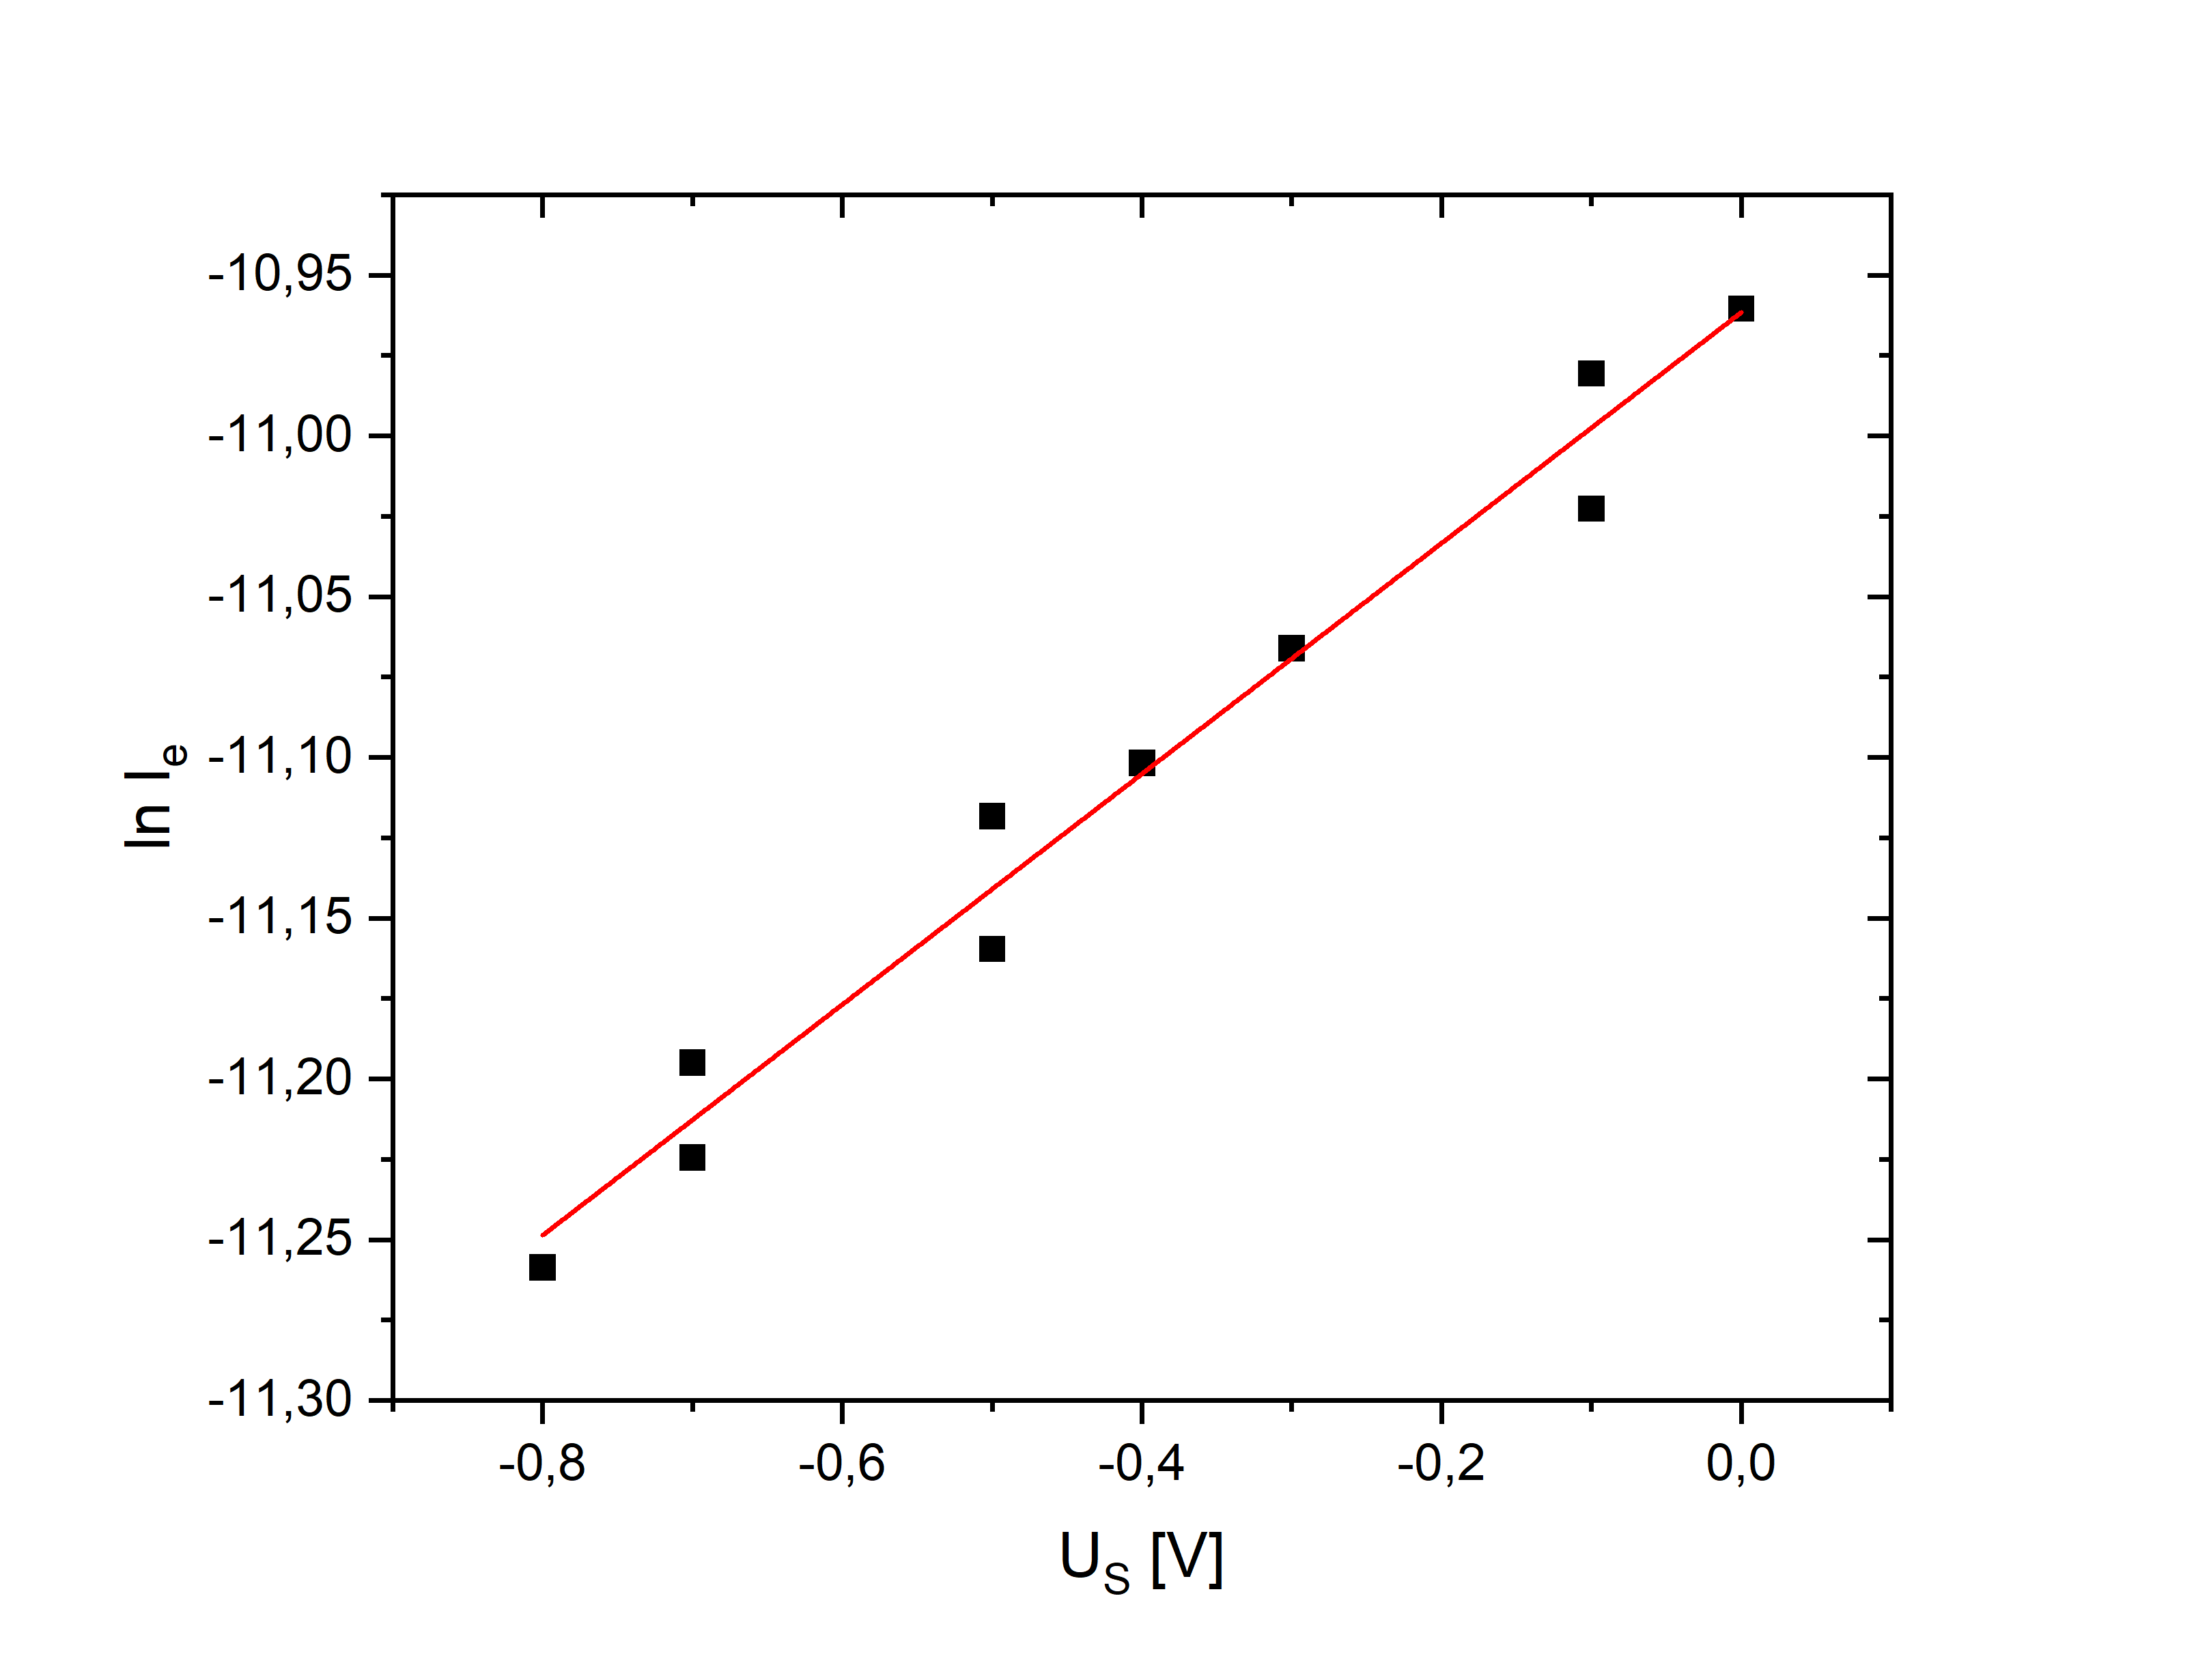
\includegraphics{data0T.png}}
		%\caption{$f(t) = \ln n$}
	\end{subfigure}
	\caption{Stanovení potenciálu plazmatu a elektronové teploty pomocí 
		průsečíku asymptot, $p = 160$ \si{\pascal} a 
	$I_\text{v} = 40$ \si{\milli\ampere}.}
	\label{data0}
\end{figure}

\newpage
\begin{figure}[h]
	\centering
	\begin{subfigure}[b]{.49\textwidth}
		\centering
		\scalebox{.34}{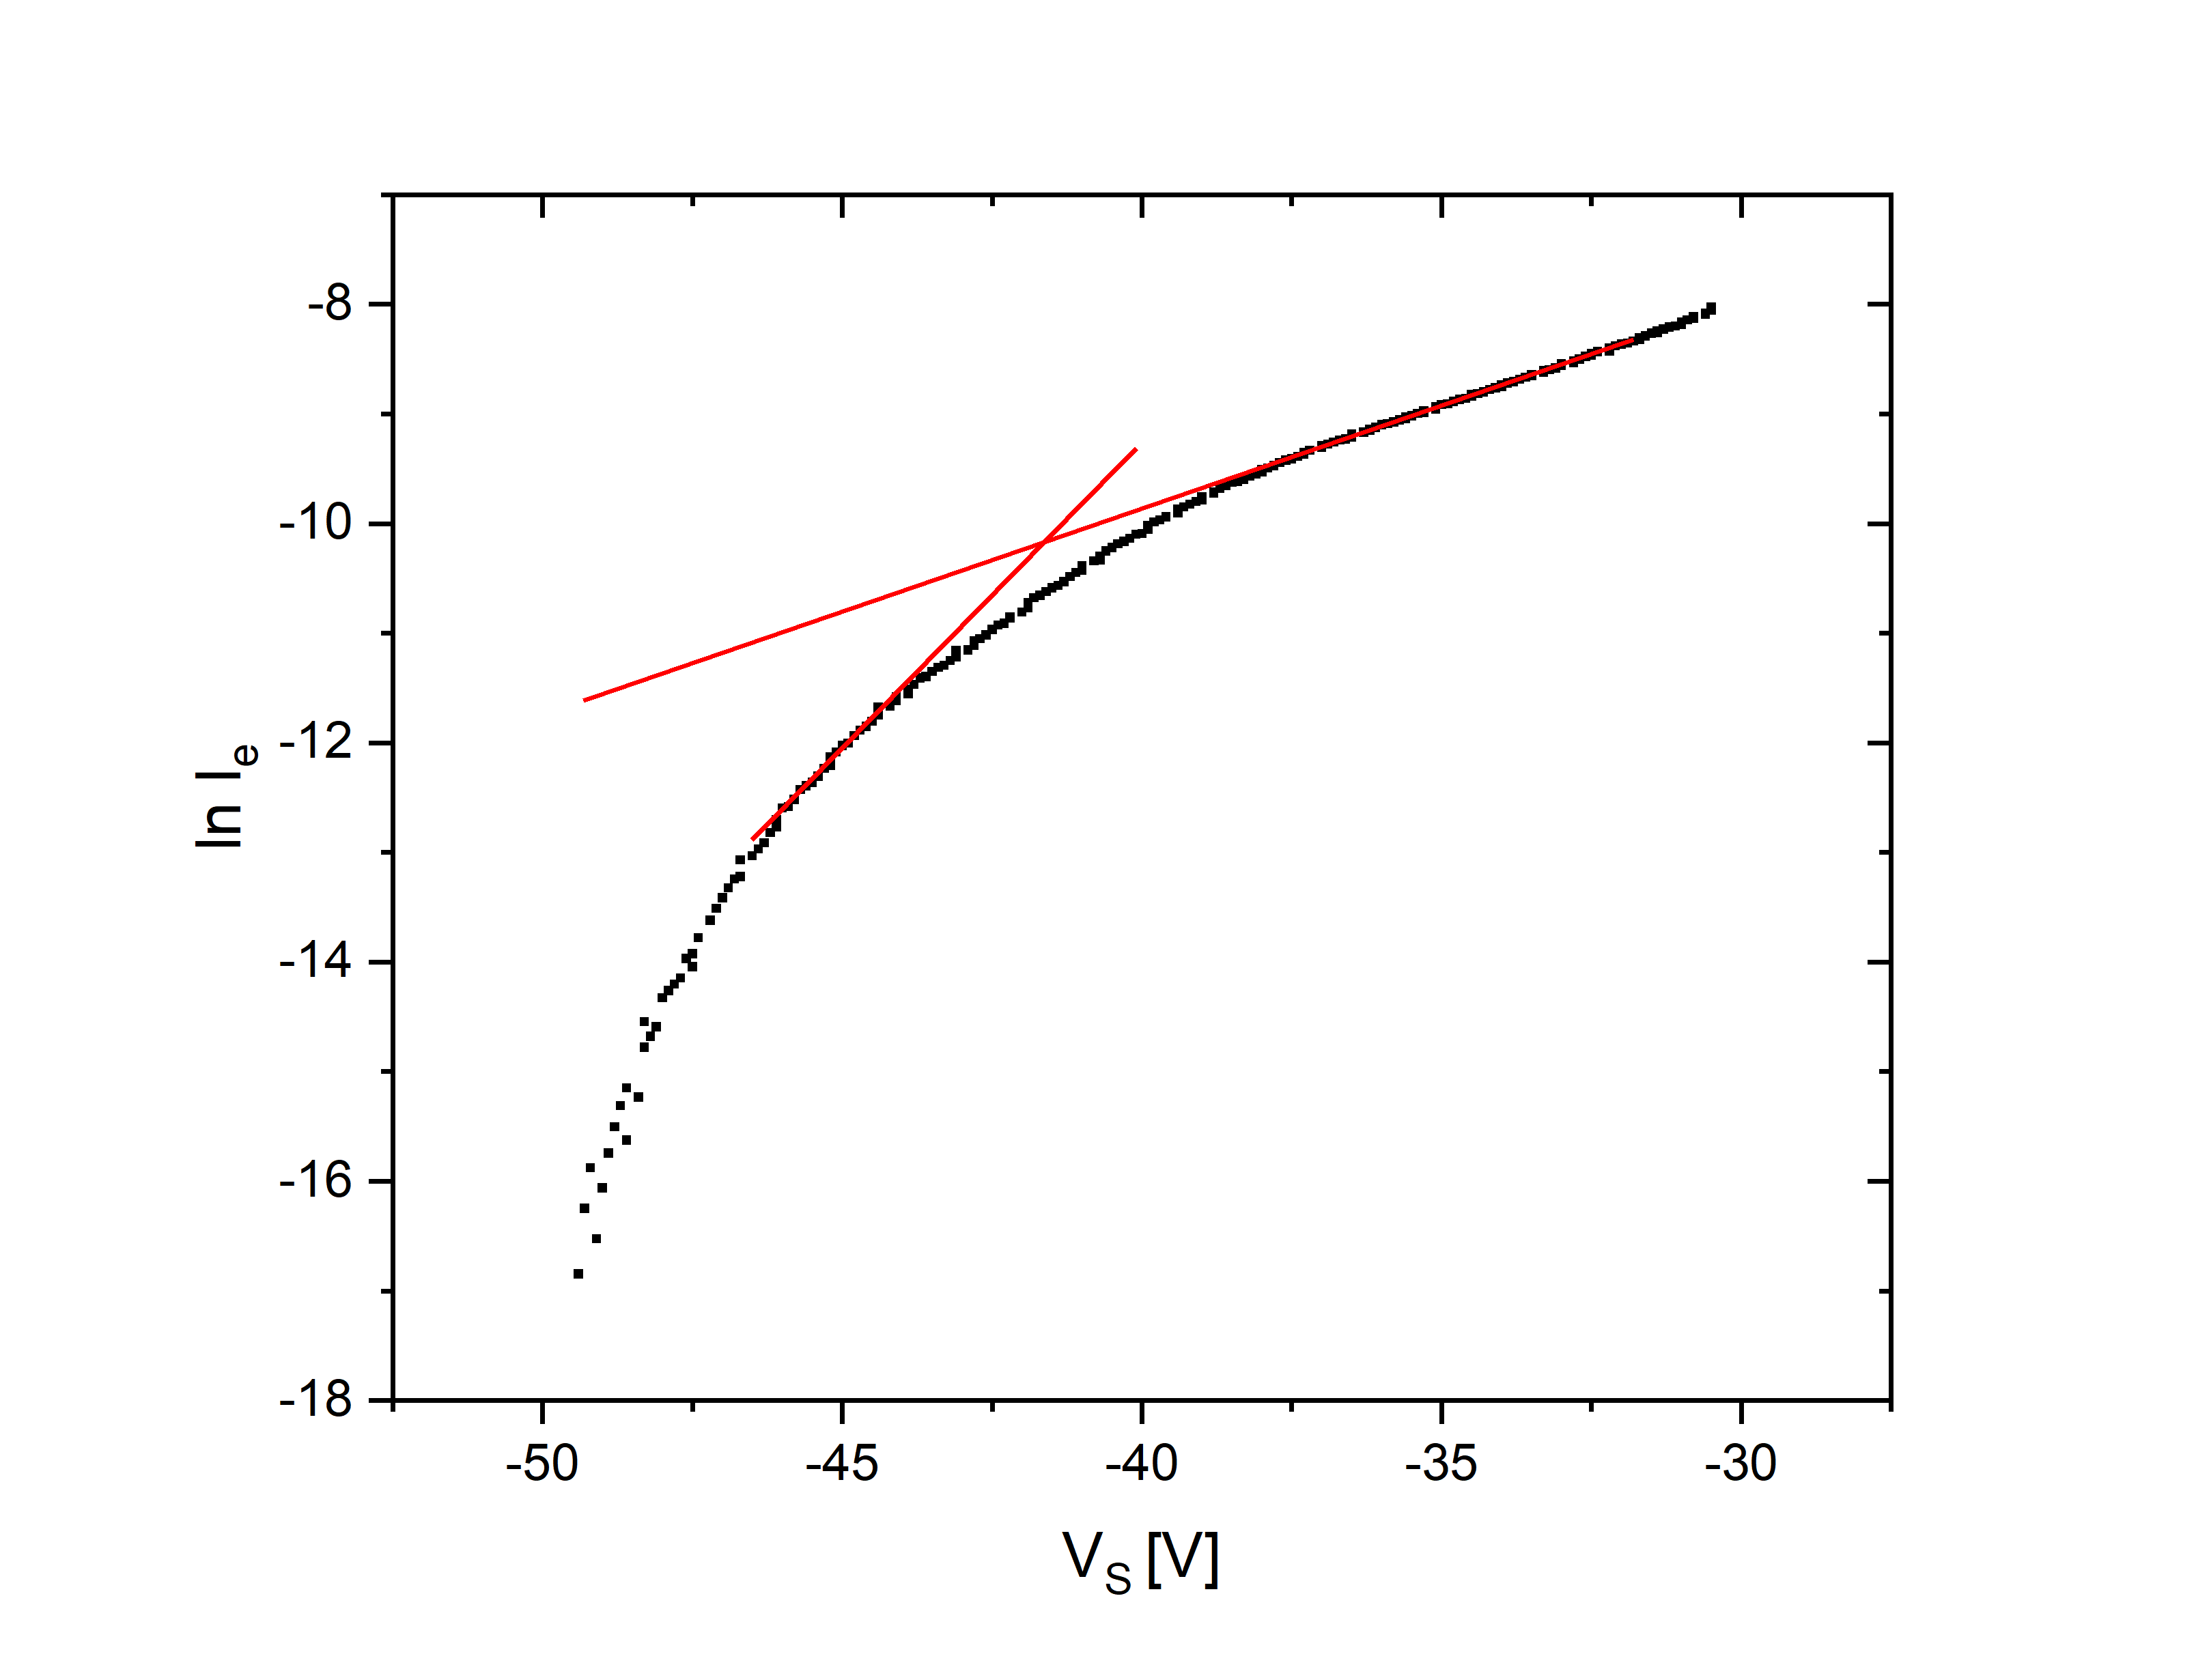
\includegraphics{data2Vp.png}}
		%\caption{$f(t) = 1/n$}
	\end{subfigure}
	\begin{subfigure}[b]{.49\textwidth}
		\centering
		\scalebox{.34}{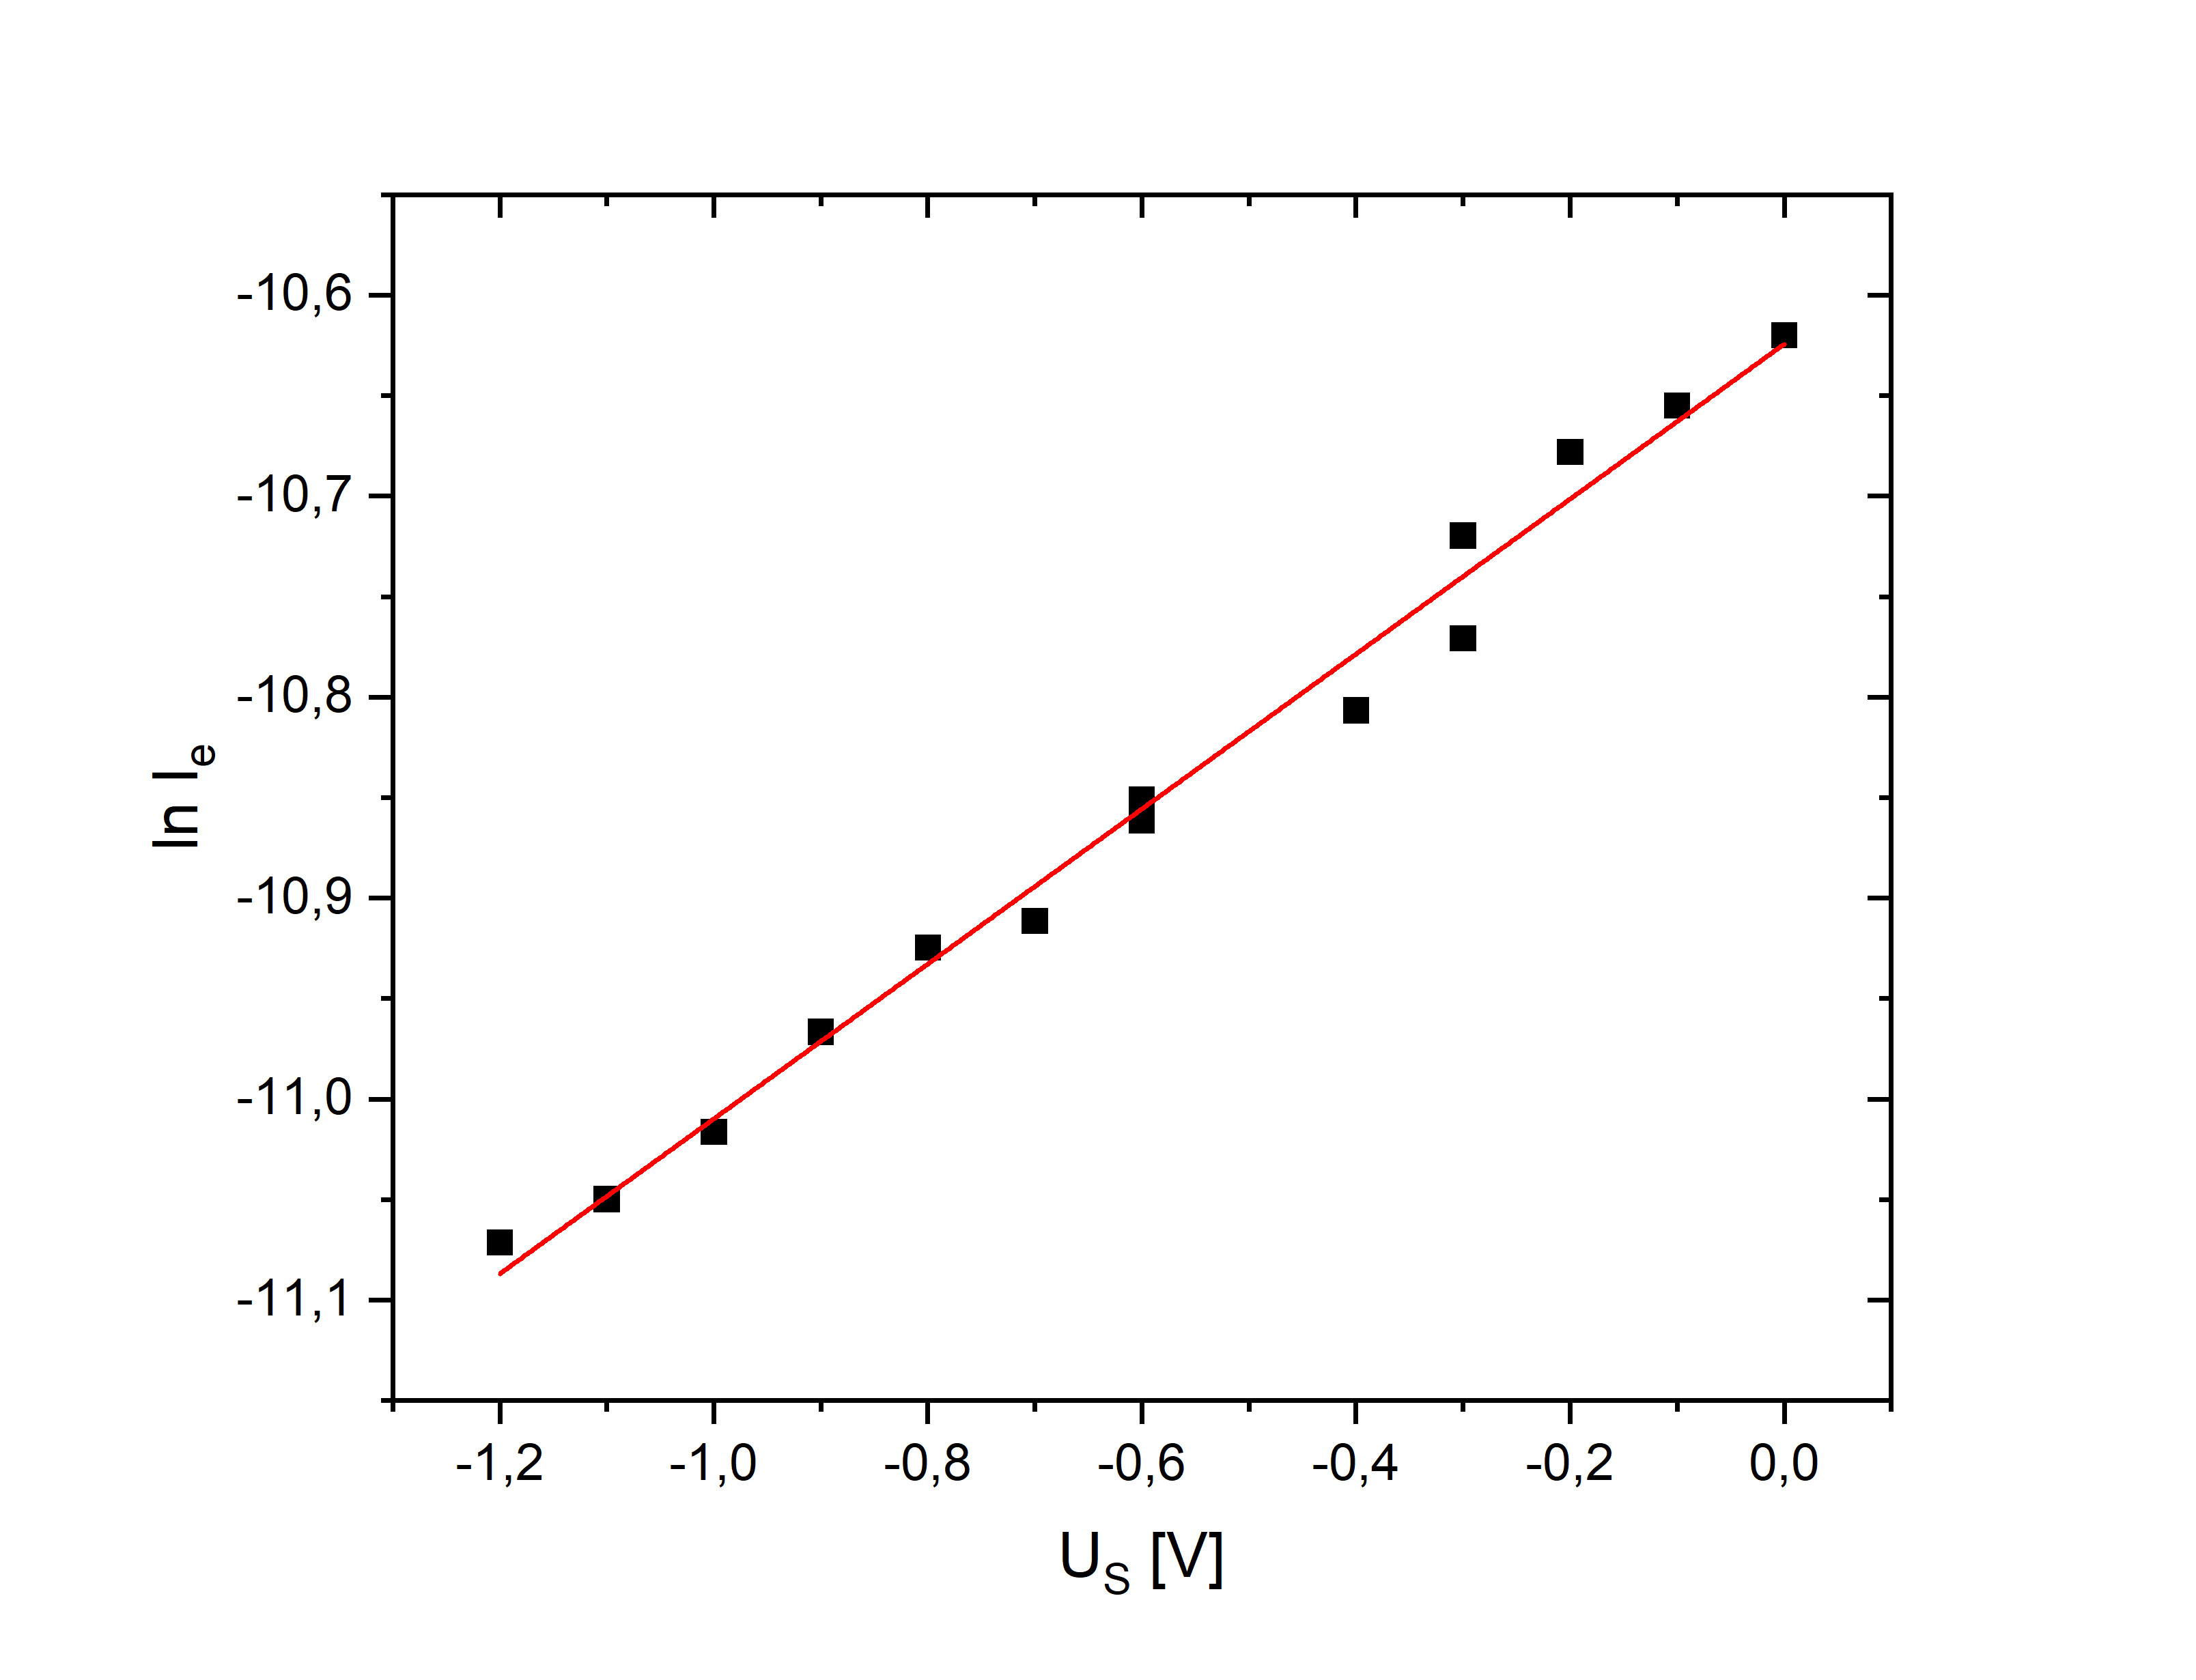
\includegraphics{data2T.png}}
		%\caption{$f(t) = \ln n$}
	\end{subfigure}
	\caption{Stanovení potenciálu plazmatu a elektronové teploty pomocí 
		průsečíku asymptot, $p = 160$ \si{\pascal} a $I_\text{v} = 50$ 
		\si{\milli\ampere}.}
	\label{data2}
\end{figure}



\begin{figure}[h]
	\centering
	\begin{subfigure}[b]{.49\textwidth}
		\centering
		\scalebox{.34}{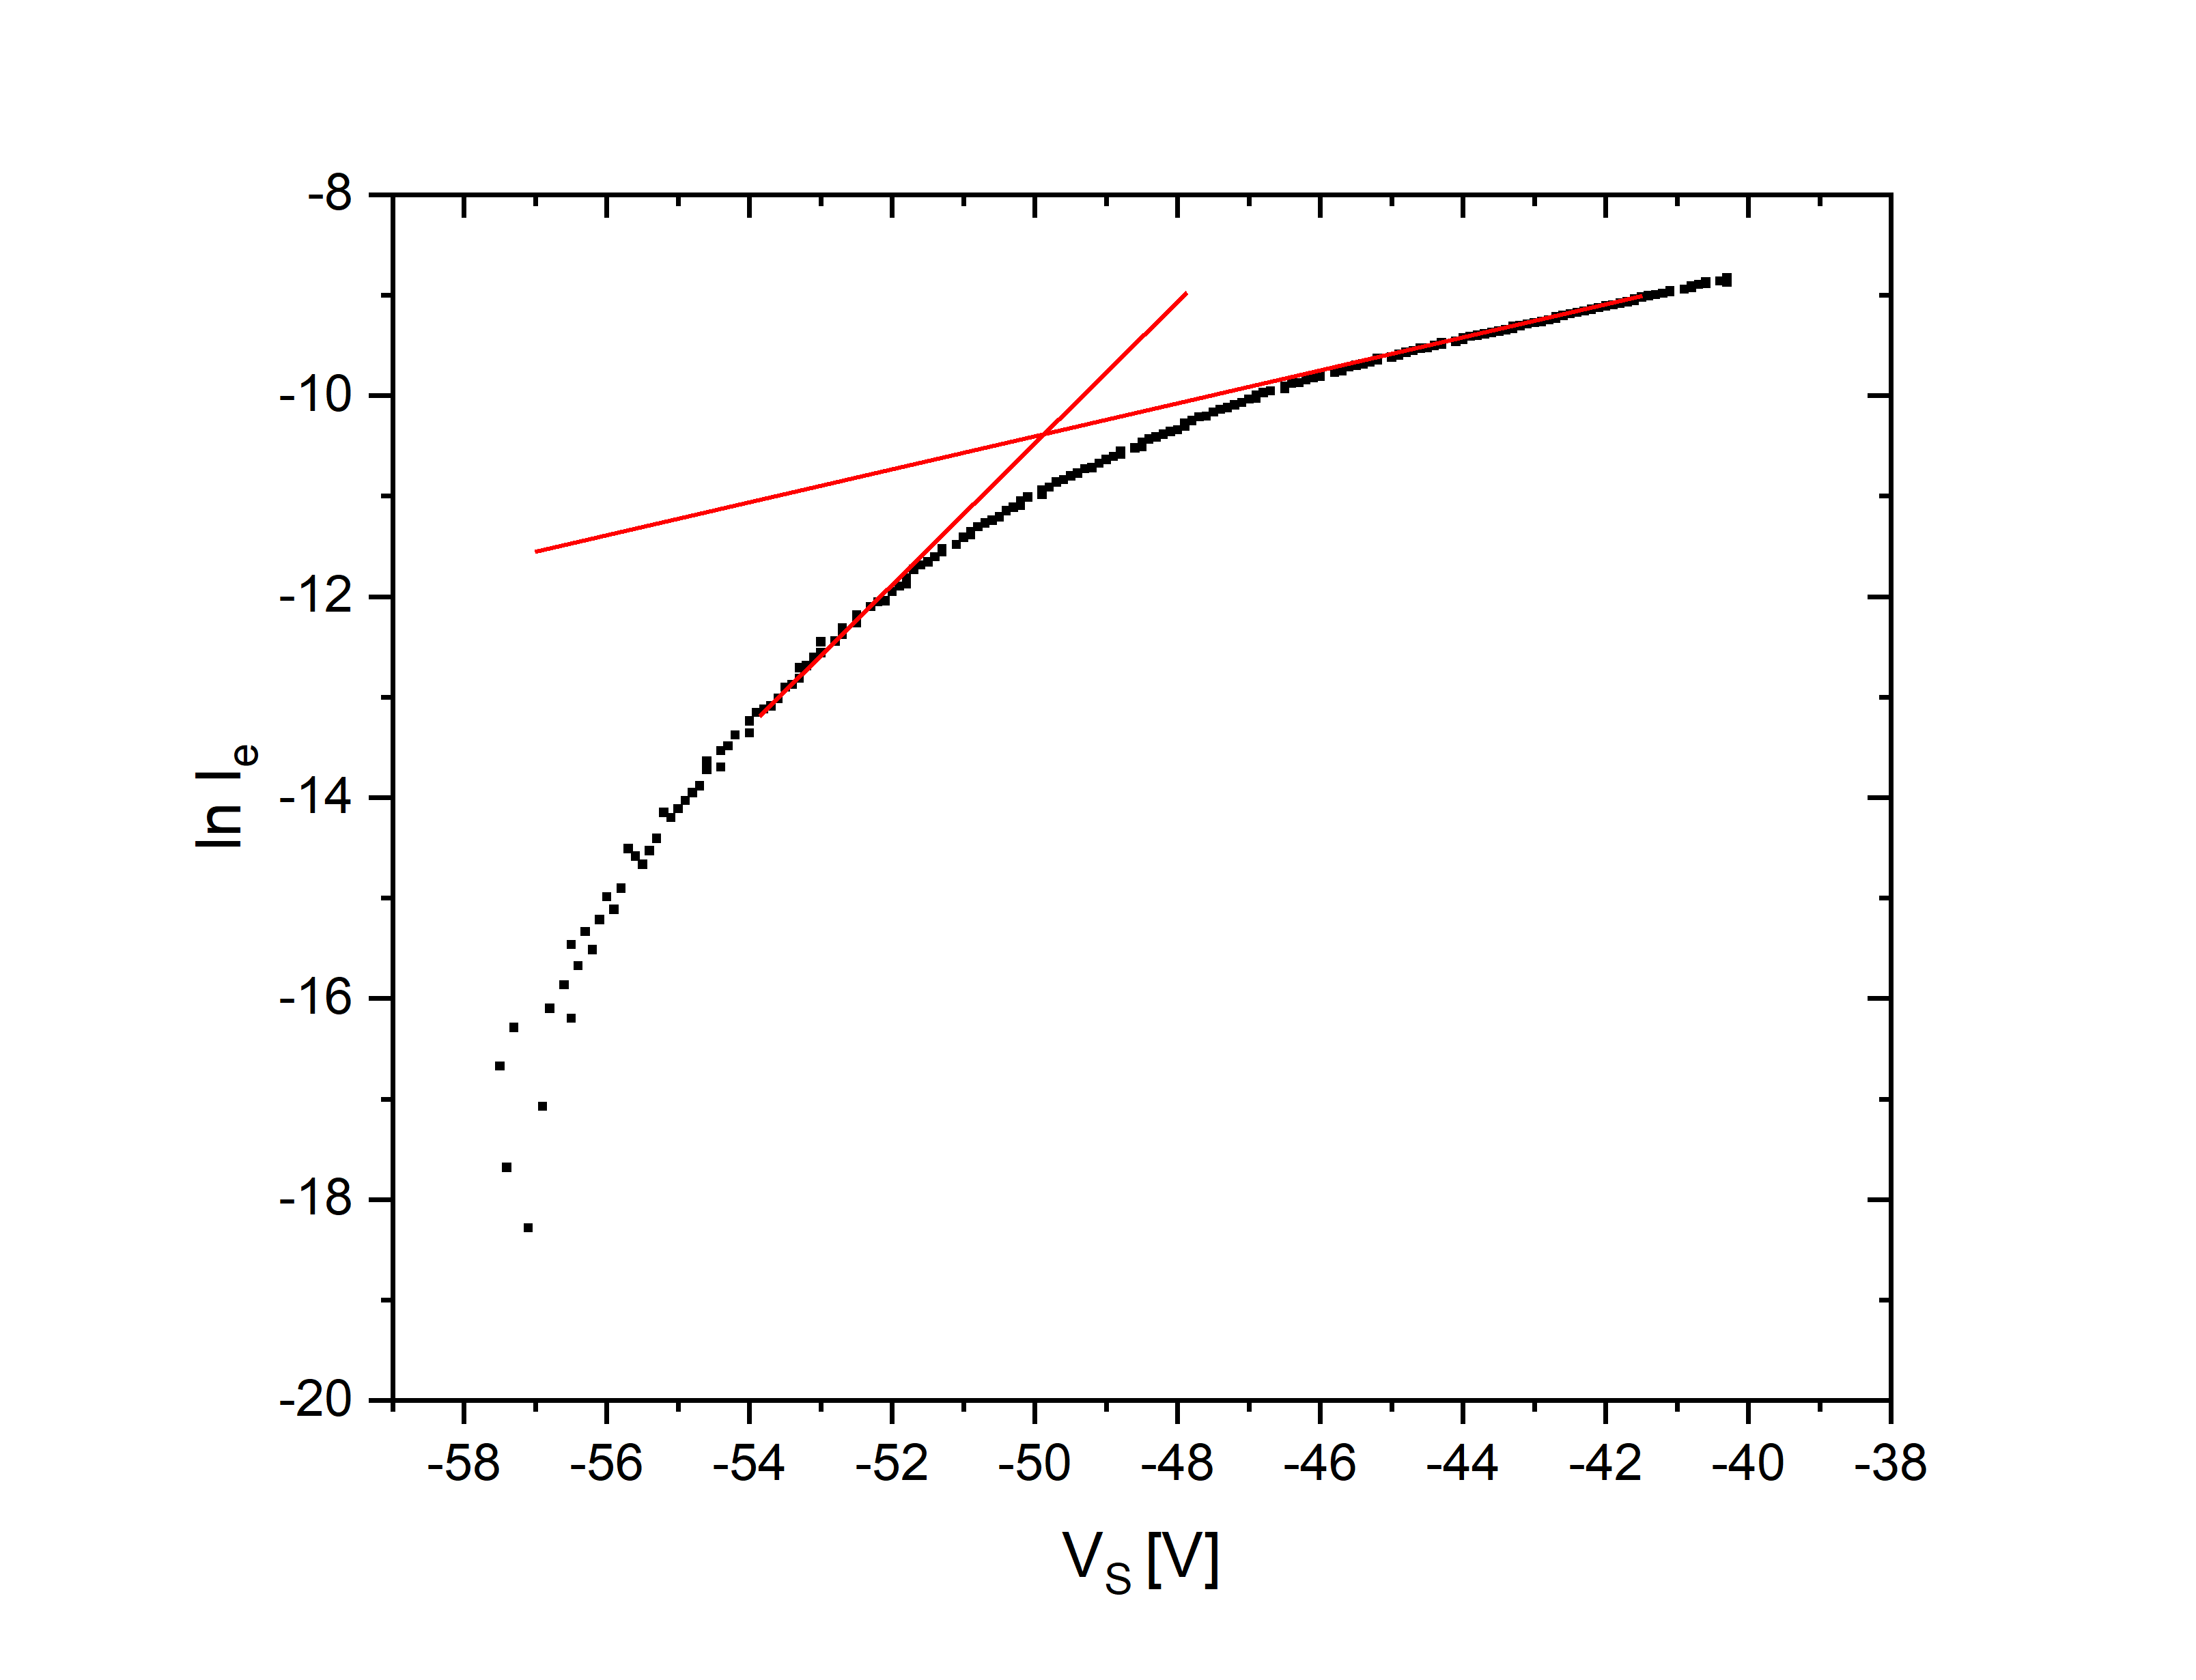
\includegraphics{data3Vp.png}}
		%\caption{$f(t) = 1/n$}
	\end{subfigure}
	\begin{subfigure}[b]{.49\textwidth}
		\centering
		\scalebox{.34}{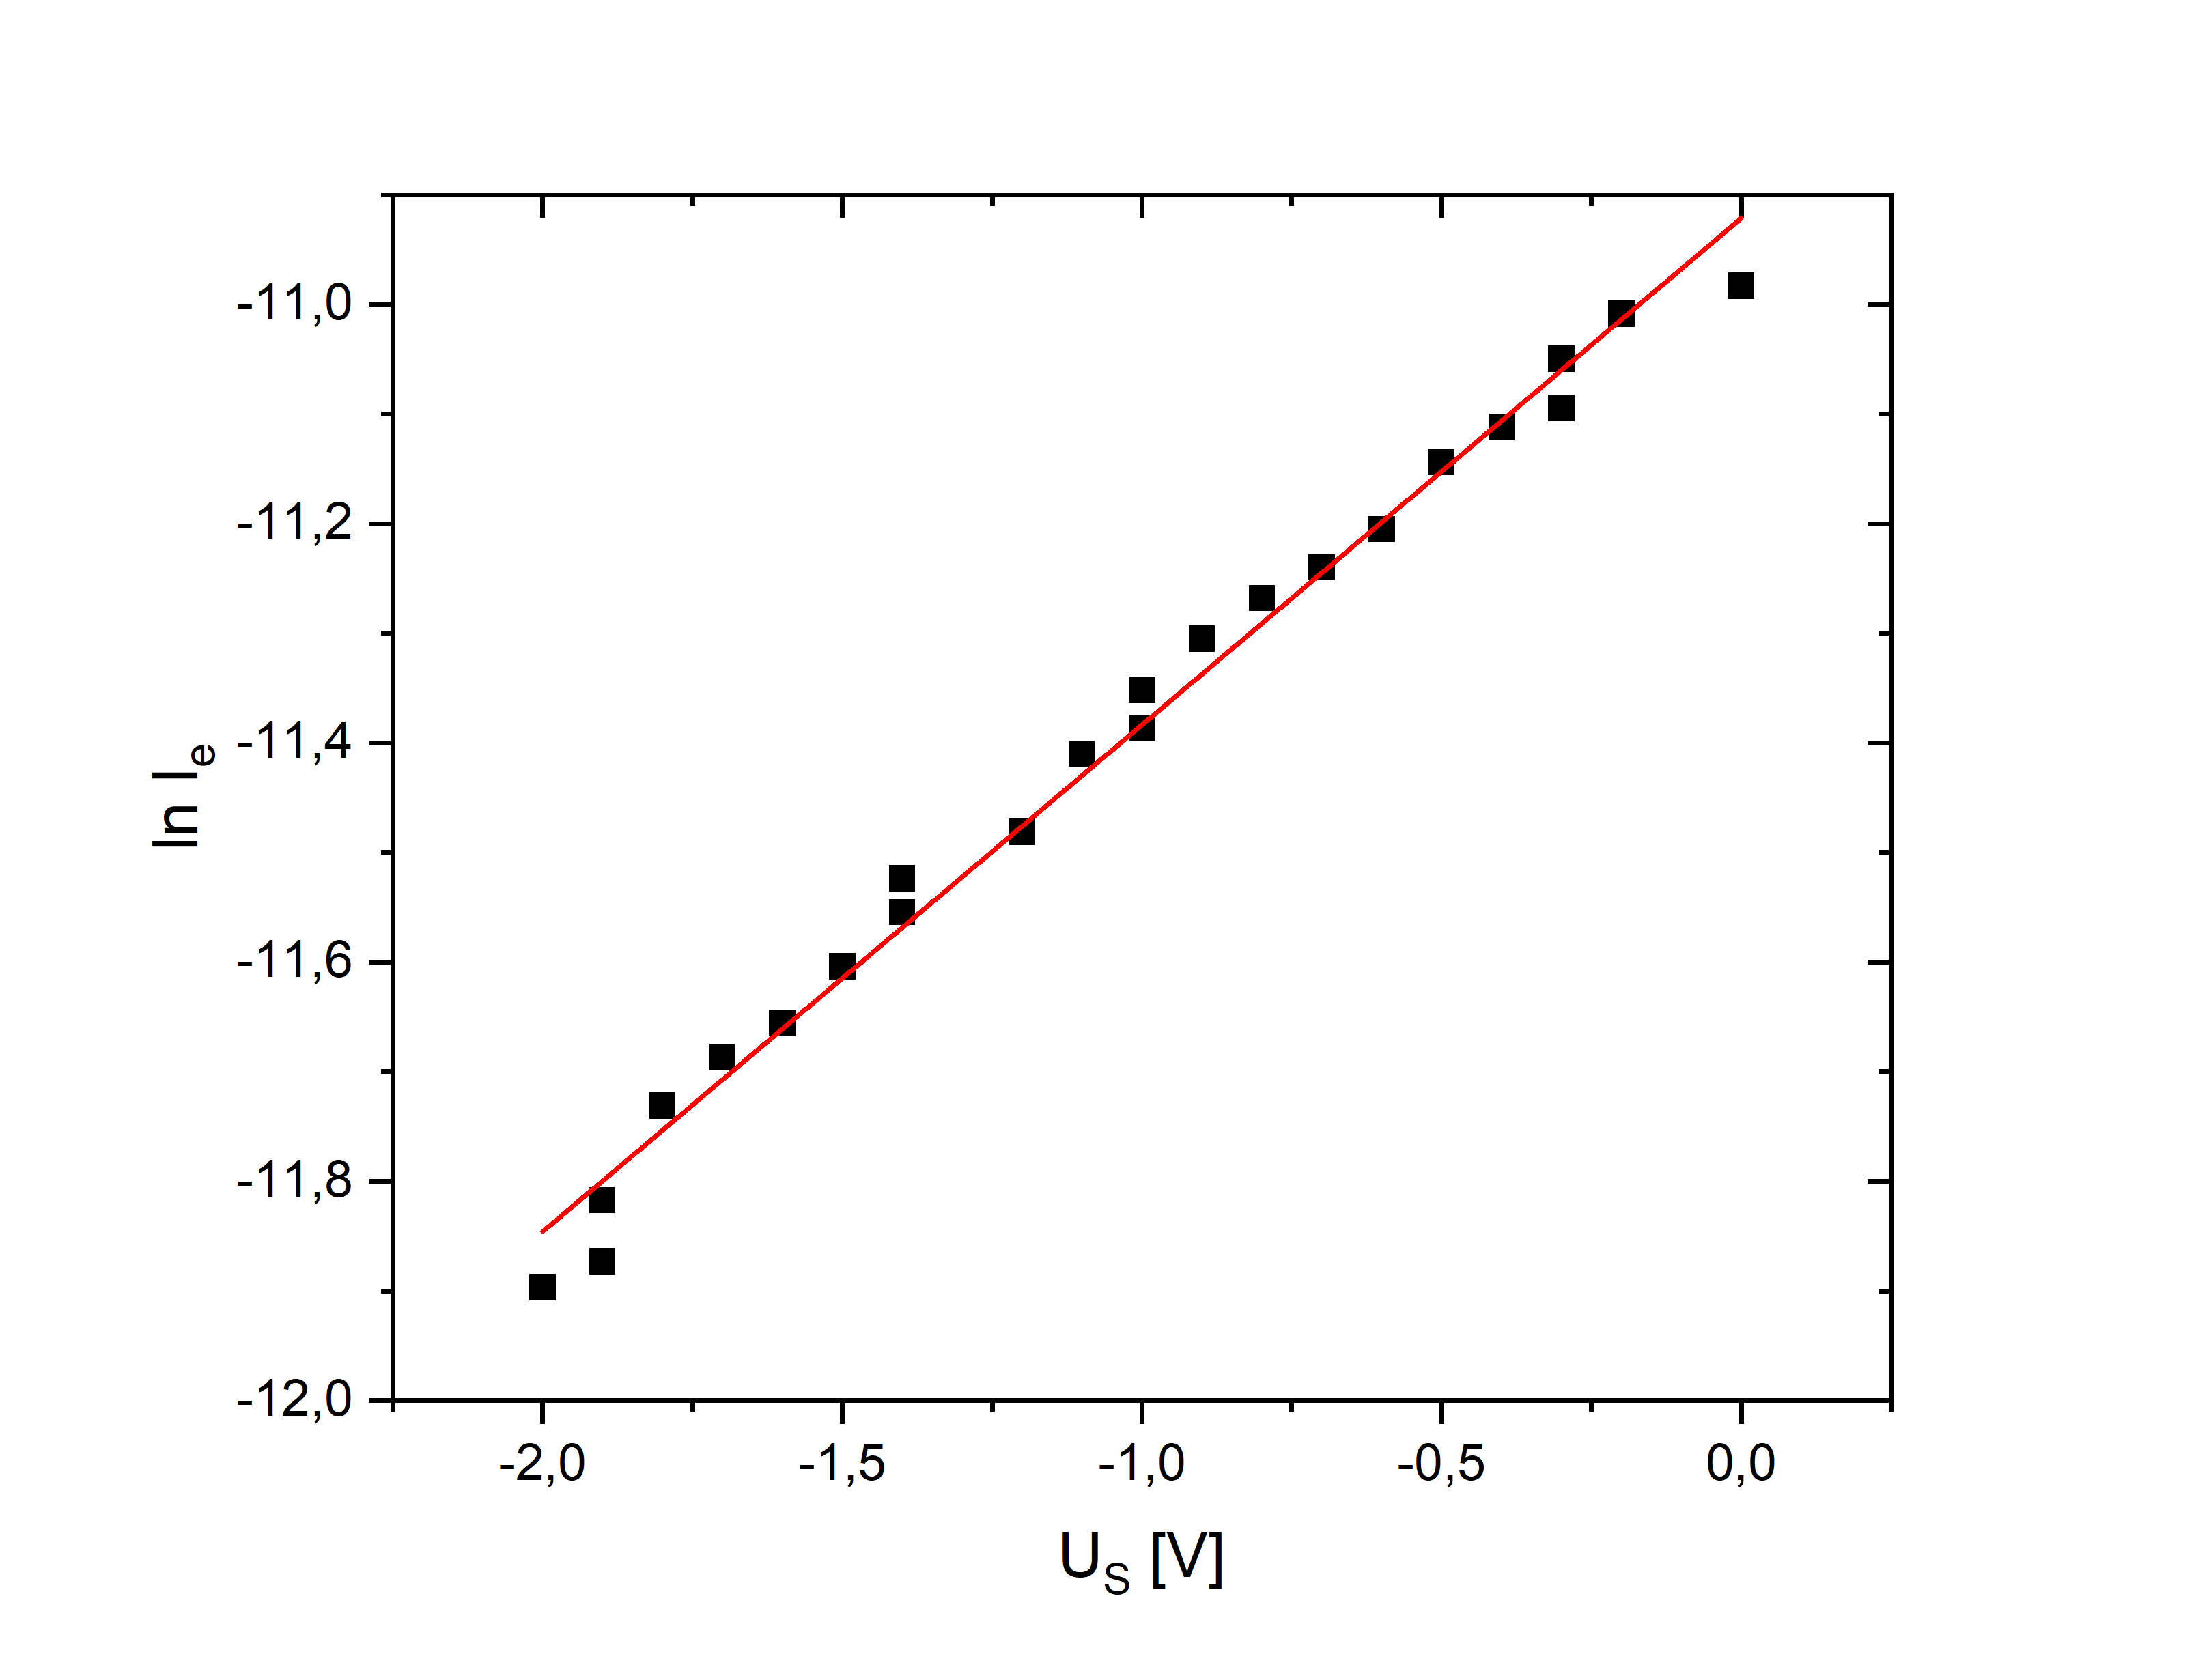
\includegraphics{data3T.png}}
		%\caption{$f(t) = \ln n$}
	\end{subfigure}
	\caption{Stanovení potenciálu plazmatu a elektronové teploty pomocí 
		průsečíku asymptot, $p = 320$ \si{\pascal} a $I_\text{v} = 40$ 
		\si{\milli\ampere}.}
	\label{data3}
\end{figure}

\newpage
\begin{figure}[h]
	\centering
	\begin{subfigure}[b]{.49\textwidth}
		\centering
		\scalebox{.34}{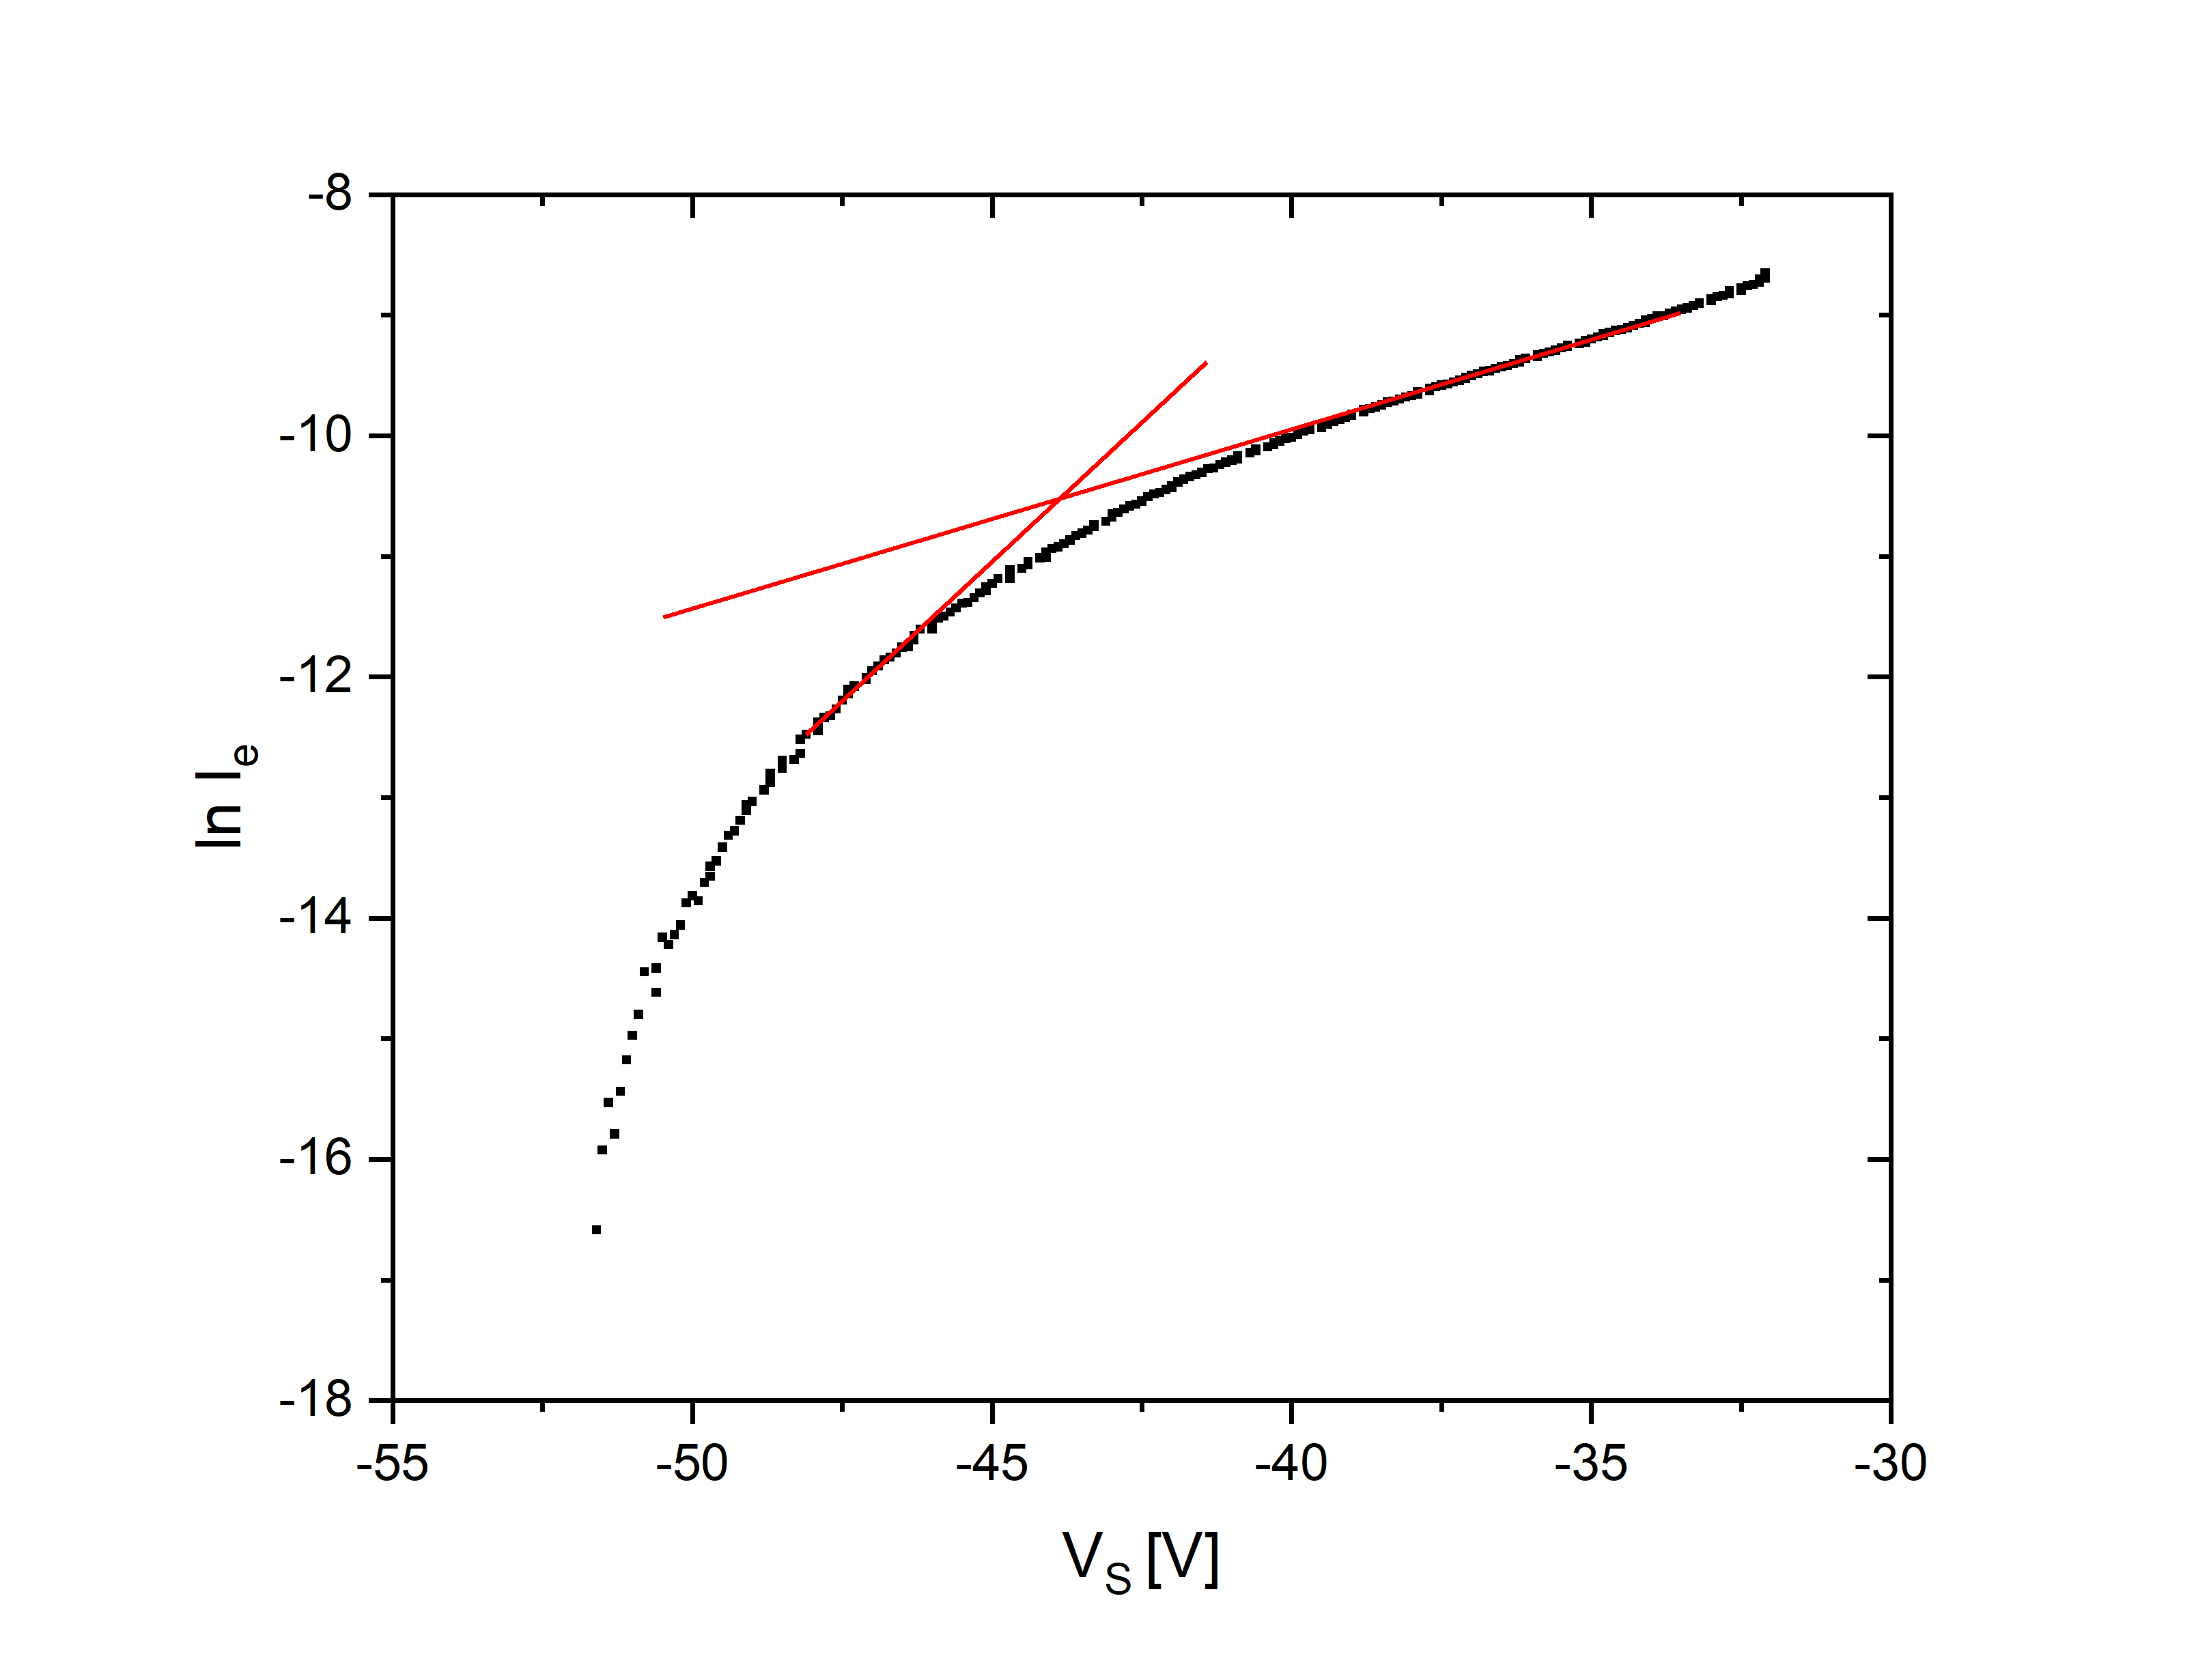
\includegraphics{data4Vp.png}}
		%\caption{$f(t) = 1/n$}
	\end{subfigure}
	\begin{subfigure}[b]{.49\textwidth}
		\centering
		\scalebox{.34}{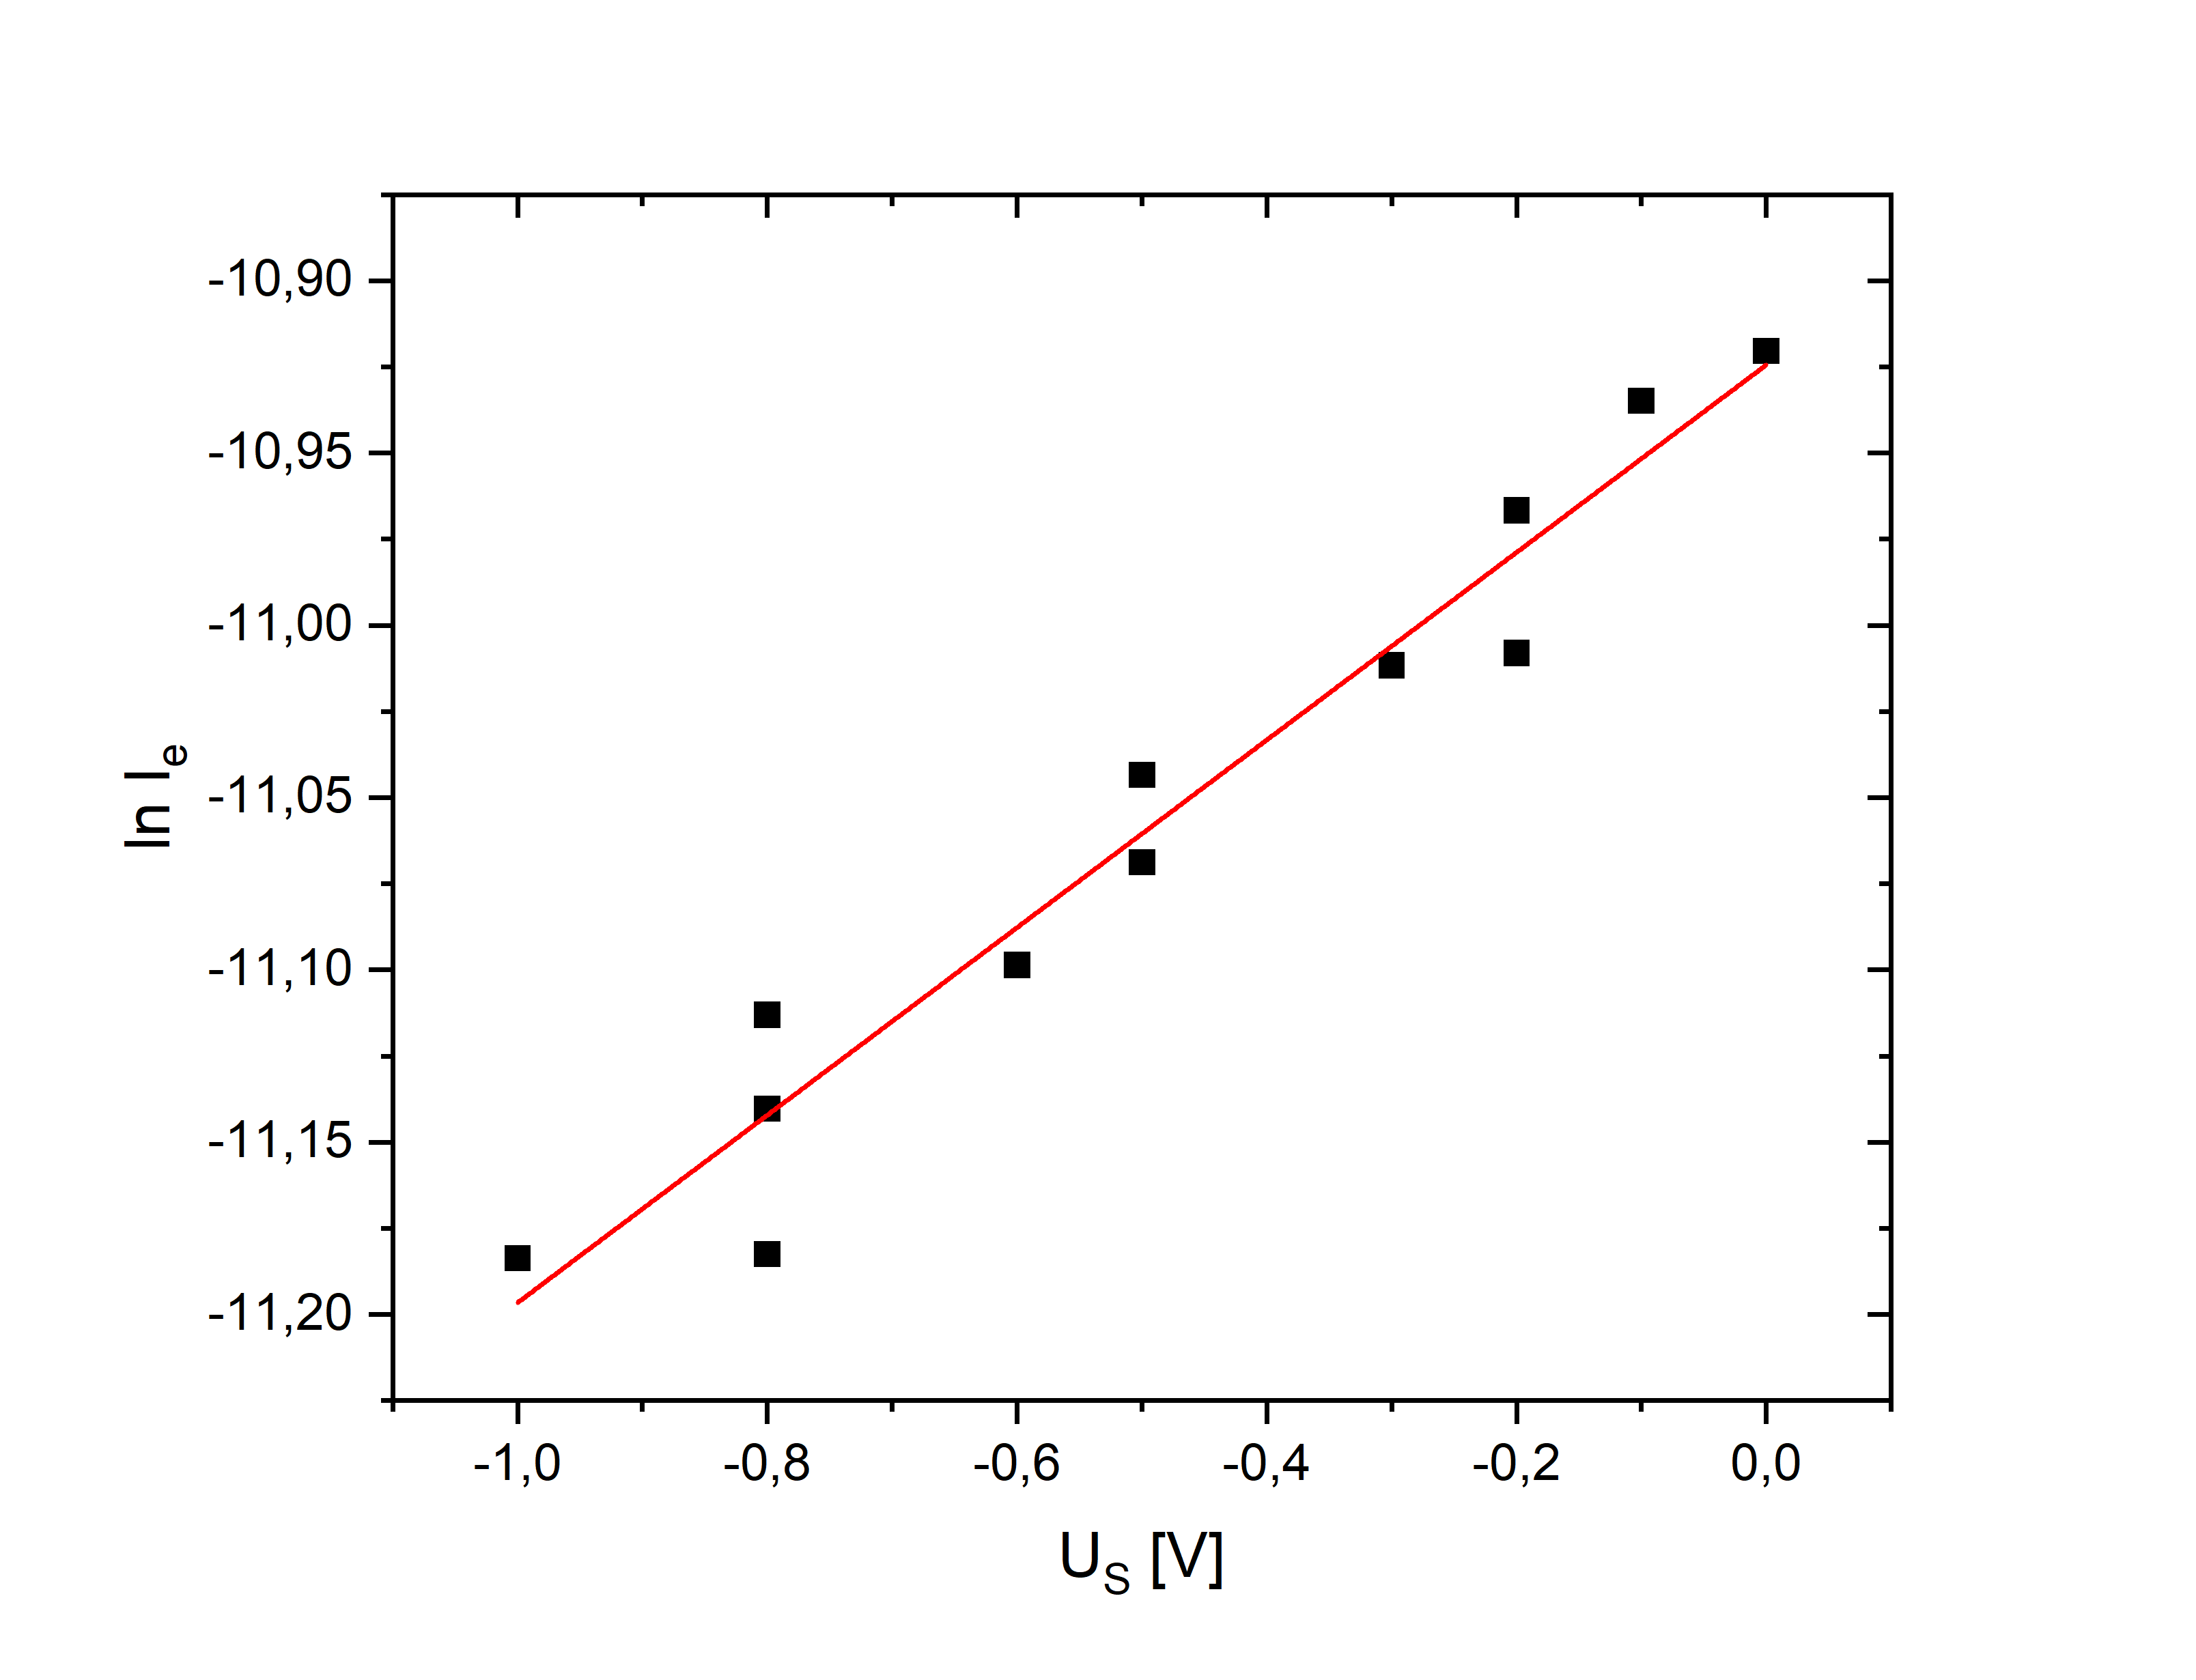
\includegraphics{data4T.png}}
		%\caption{$f(t) = \ln n$}
	\end{subfigure}
	\caption{Stanovení potenciálu plazmatu a elektronové teploty pomocí 
		průsečíku asymptot, $p = 80$ \si{\pascal} a $I_\text{v} = 40$ 
		\si{\milli\ampere}.}
	\label{data4}
\end{figure}

\begin{figure}[h]
	\centering
	\begin{subfigure}[b]{.49\textwidth}
		\centering
		\scalebox{.34}{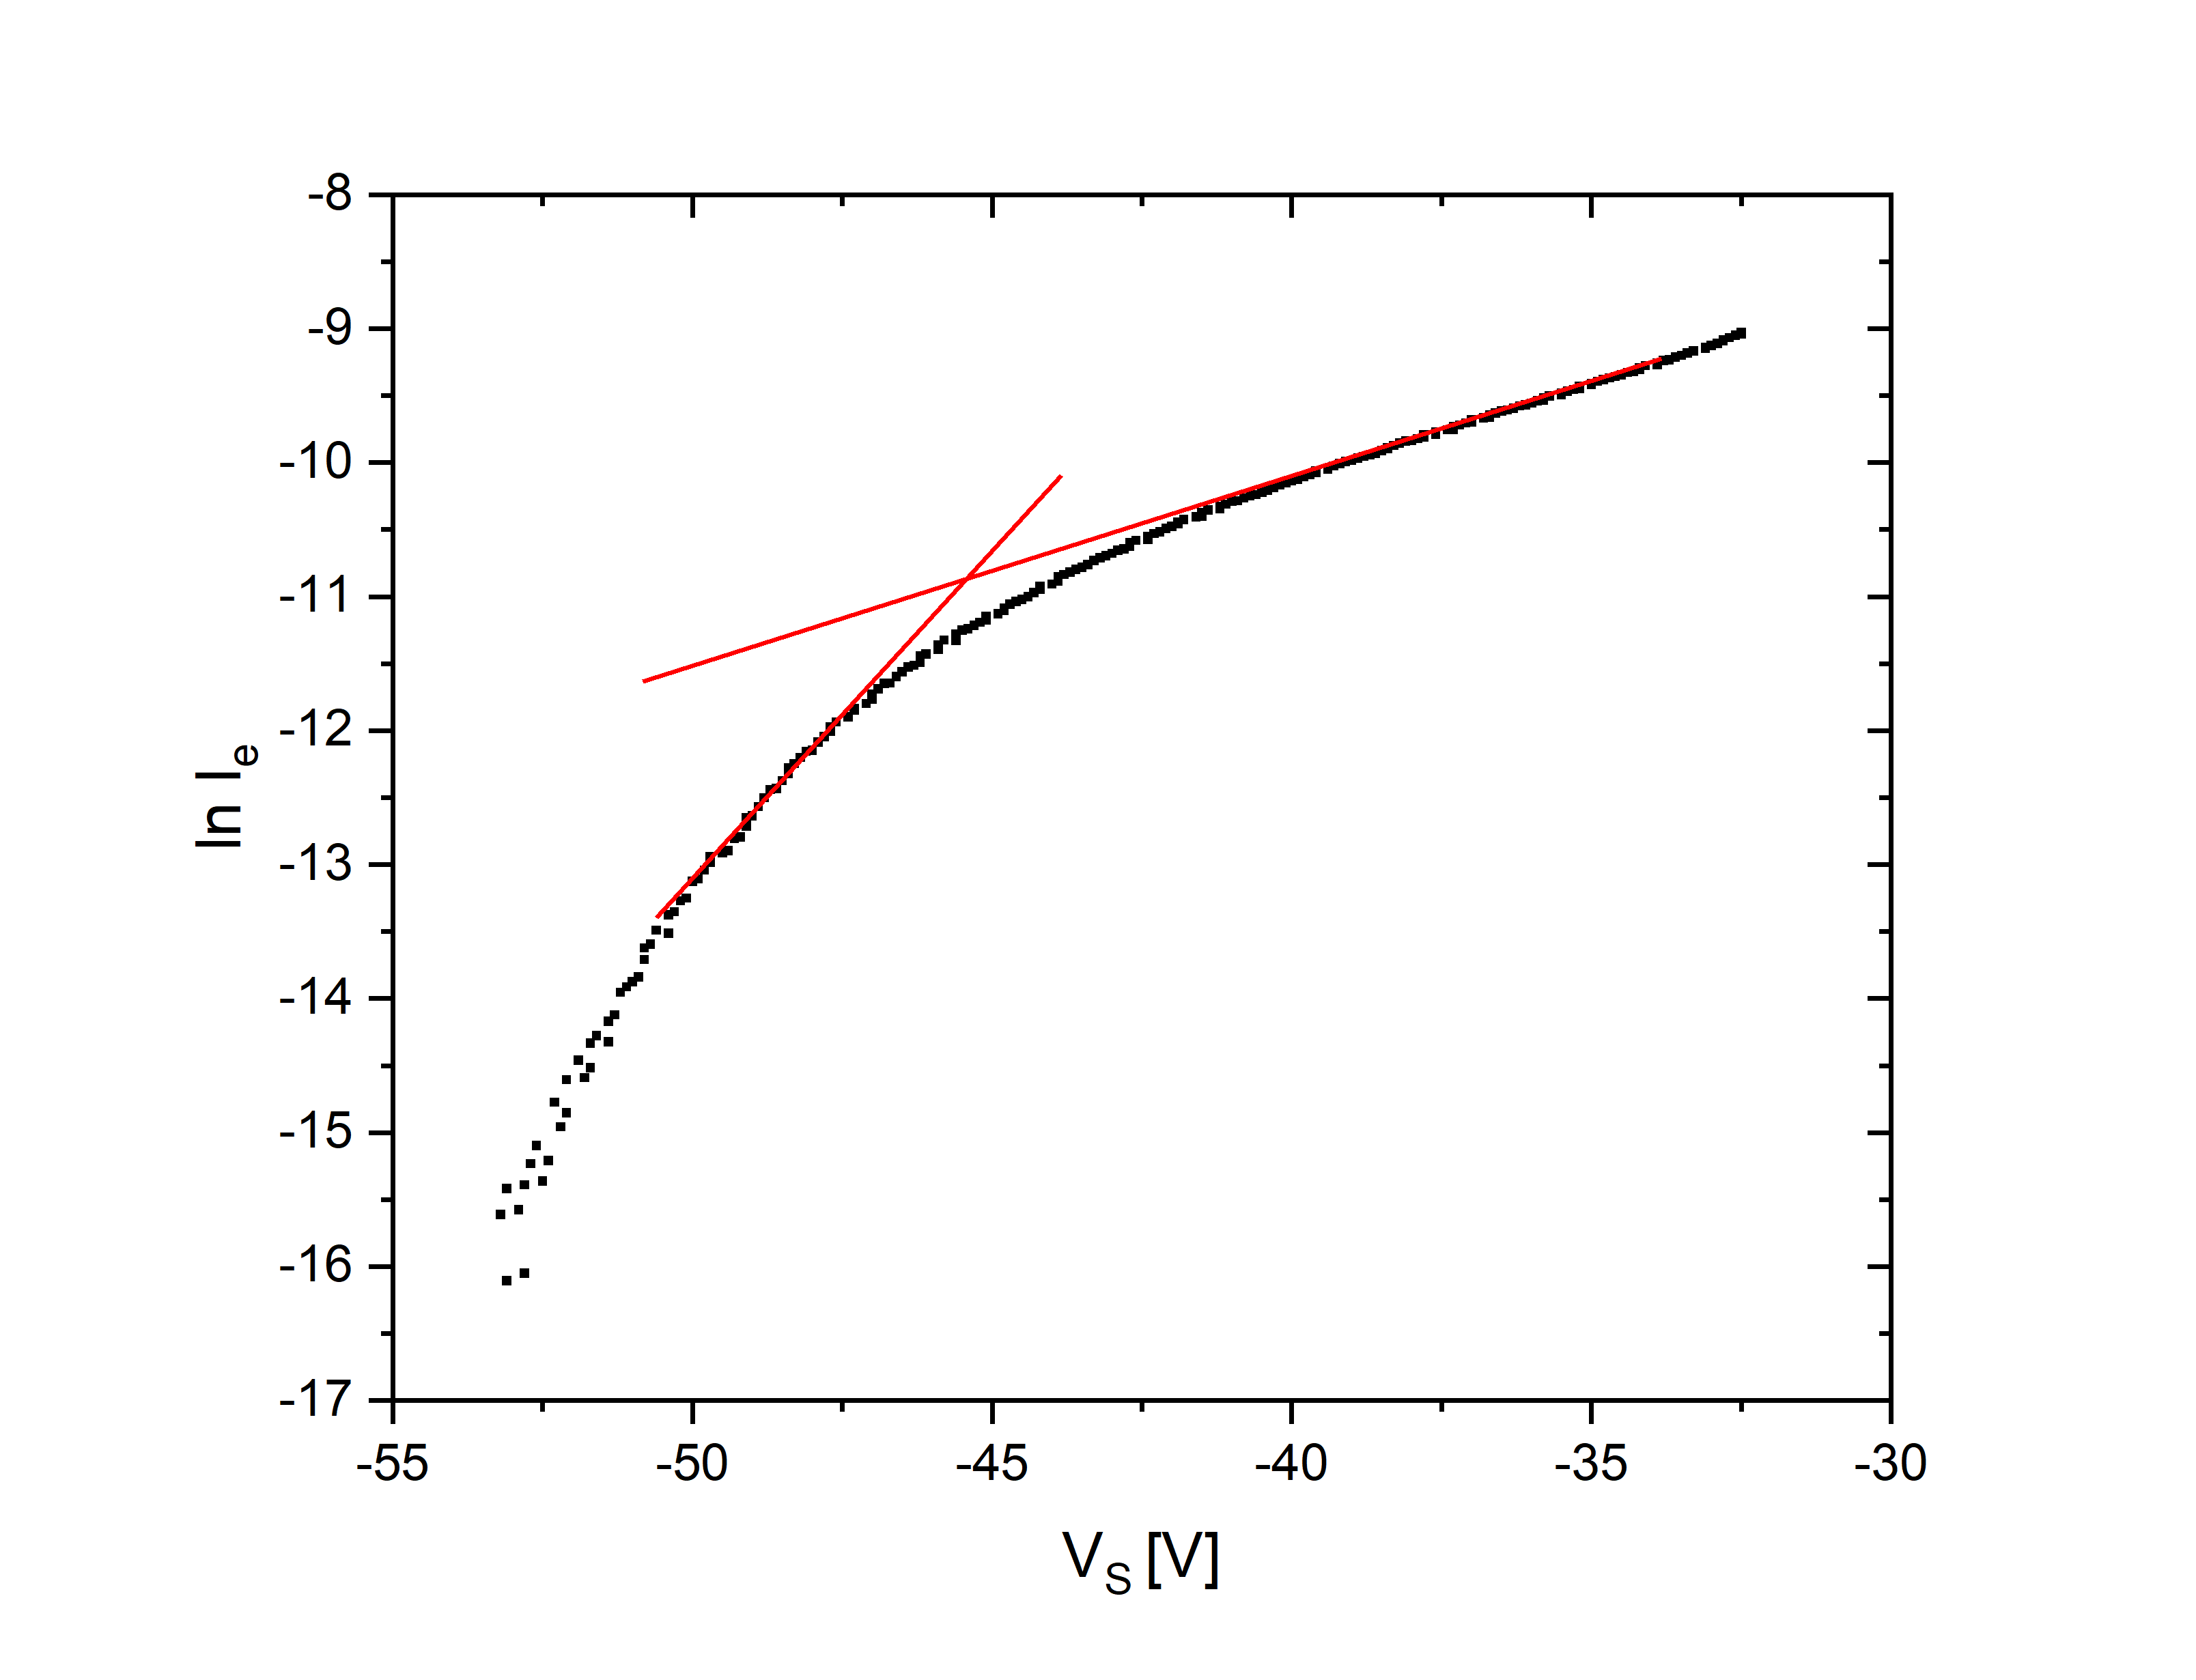
\includegraphics{data5Vp.png}}
		%\caption{$f(t) = 1/n$}
	\end{subfigure}
	\begin{subfigure}[b]{.49\textwidth}
		\centering
		\scalebox{.34}{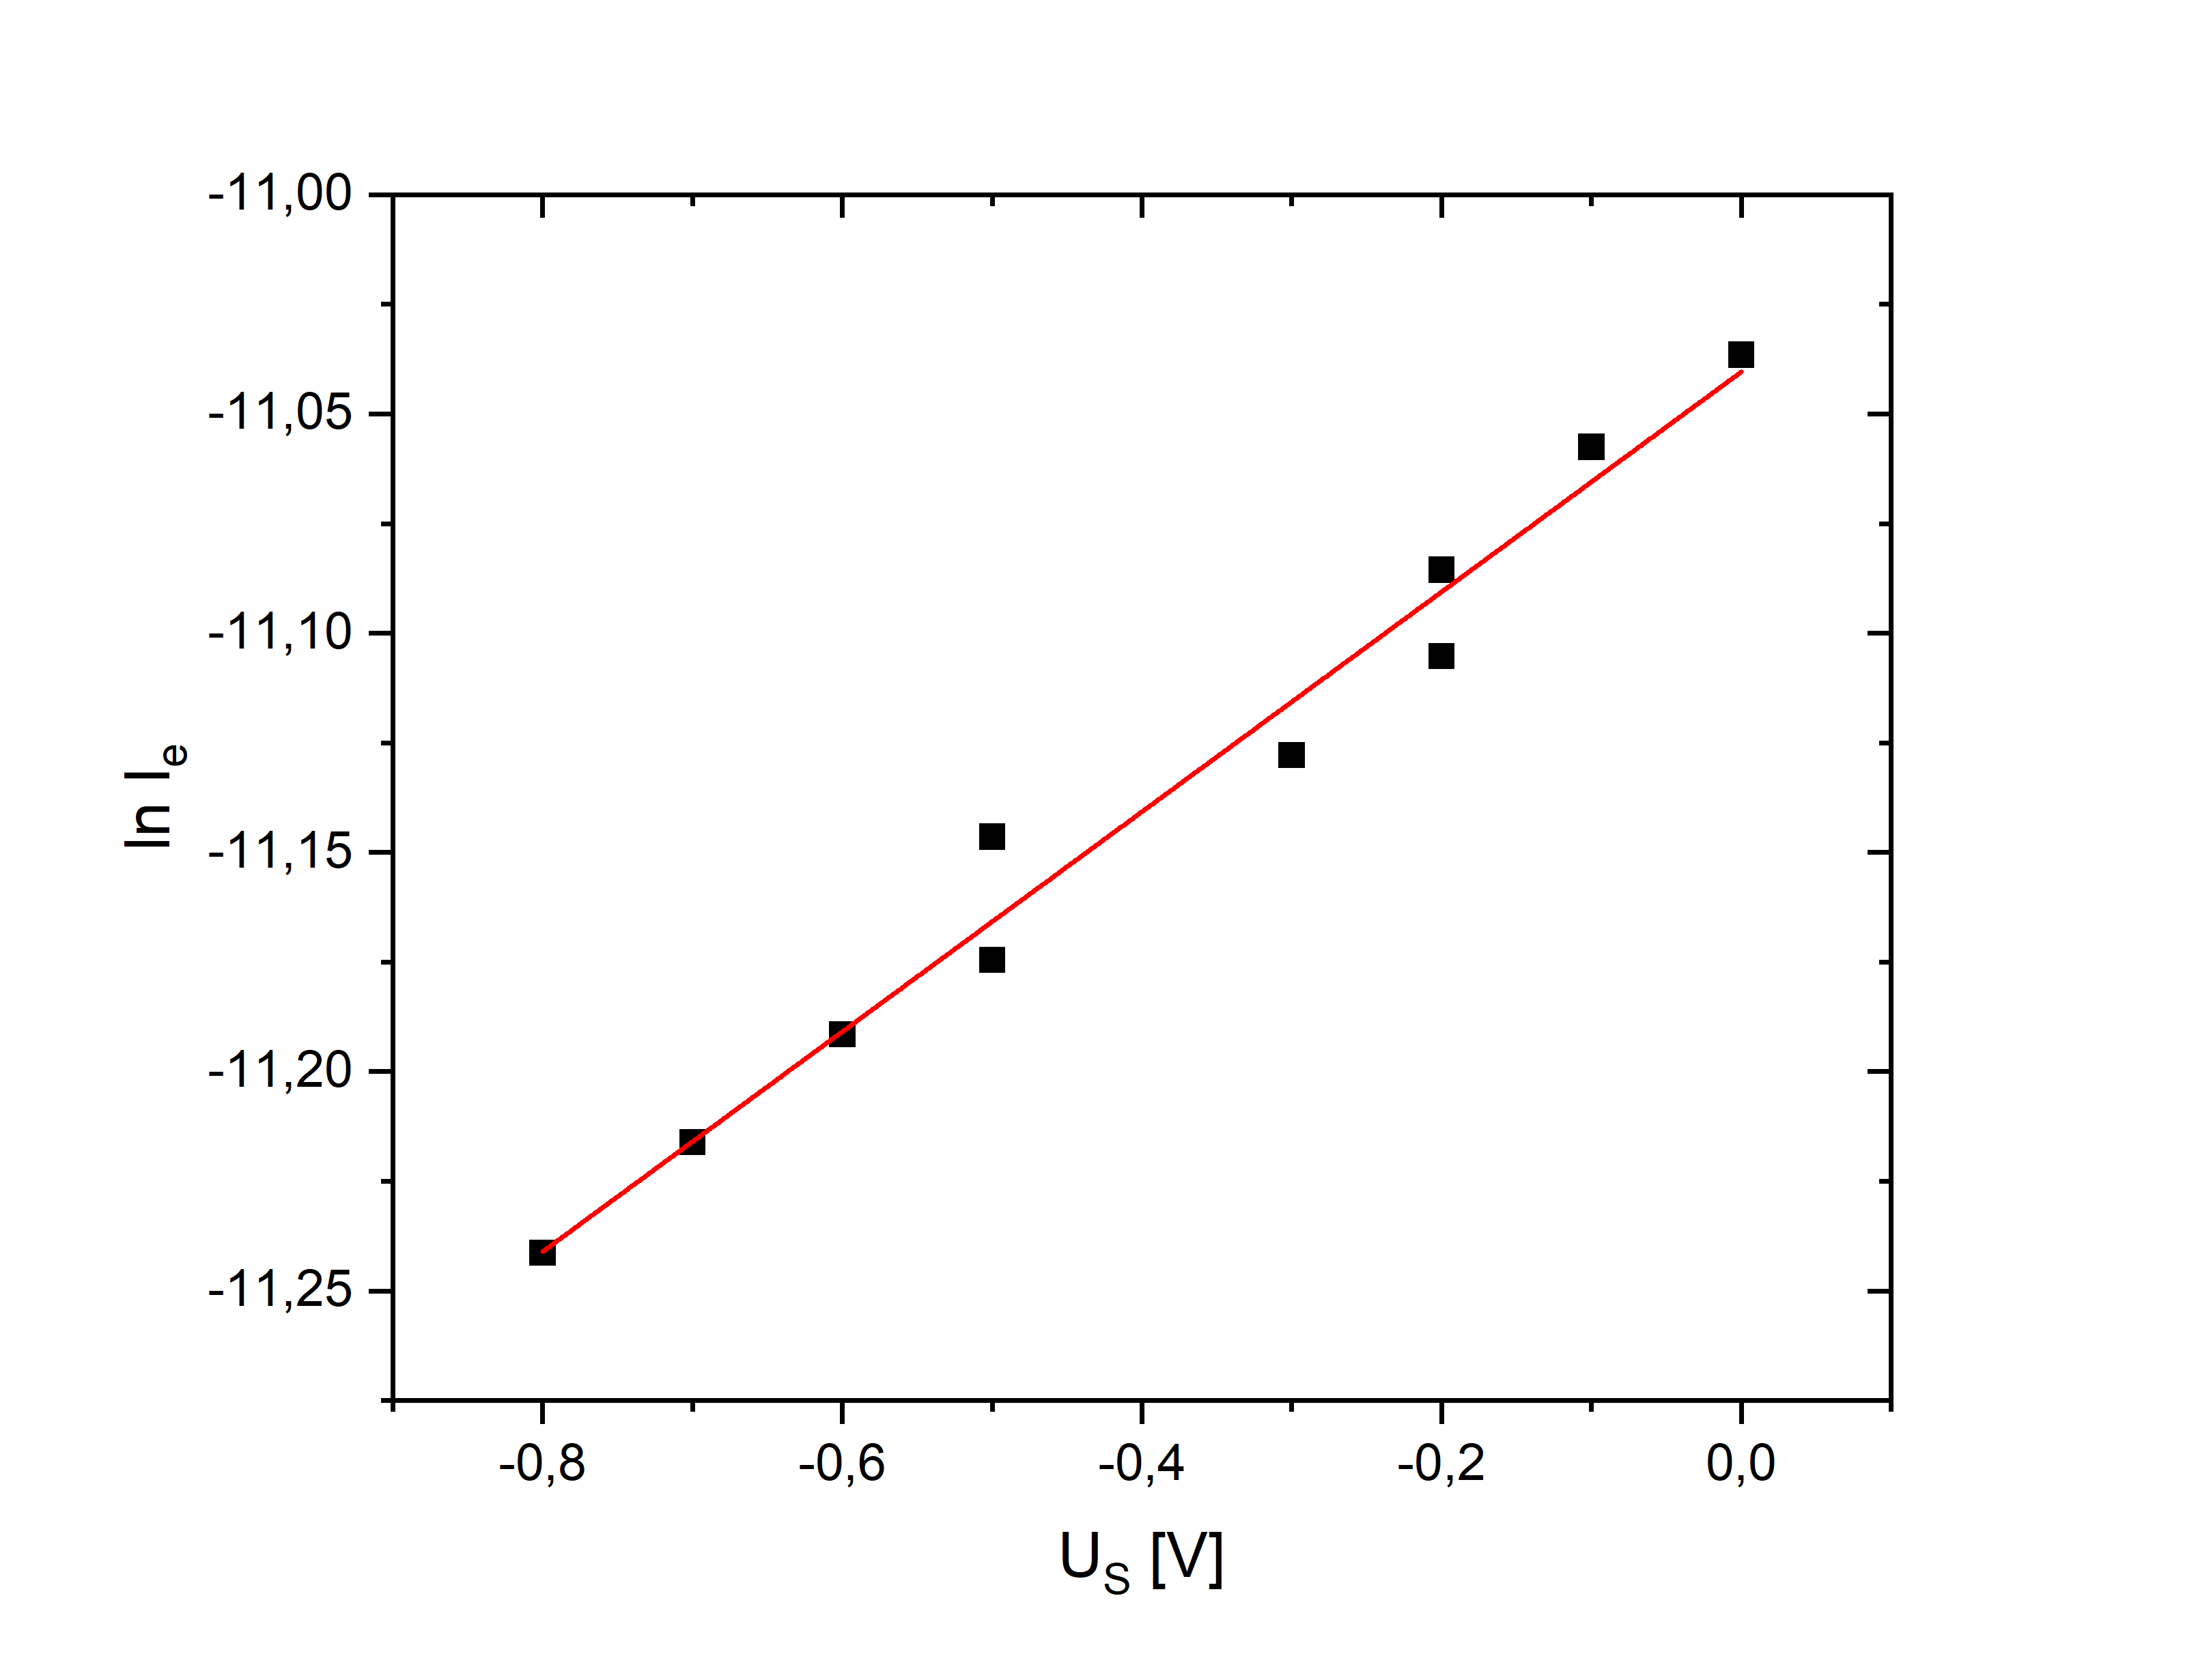
\includegraphics{data5T.png}}
		%\caption{$f(t) = \ln n$}
	\end{subfigure}
	\caption{Stanovení potenciálu plazmatu a elektronové teploty pomocí 
		průsečíku asymptot, $p = 32$ \si{\pascal} a $I_\text{v} = 40$ 
		\si{\milli\ampere}.}
	\label{data5}
\end{figure}

\newpage
\begin{figure}[h!]
	\centering
	\begin{subfigure}[b]{.49\textwidth}
		\centering
		\scalebox{.34}{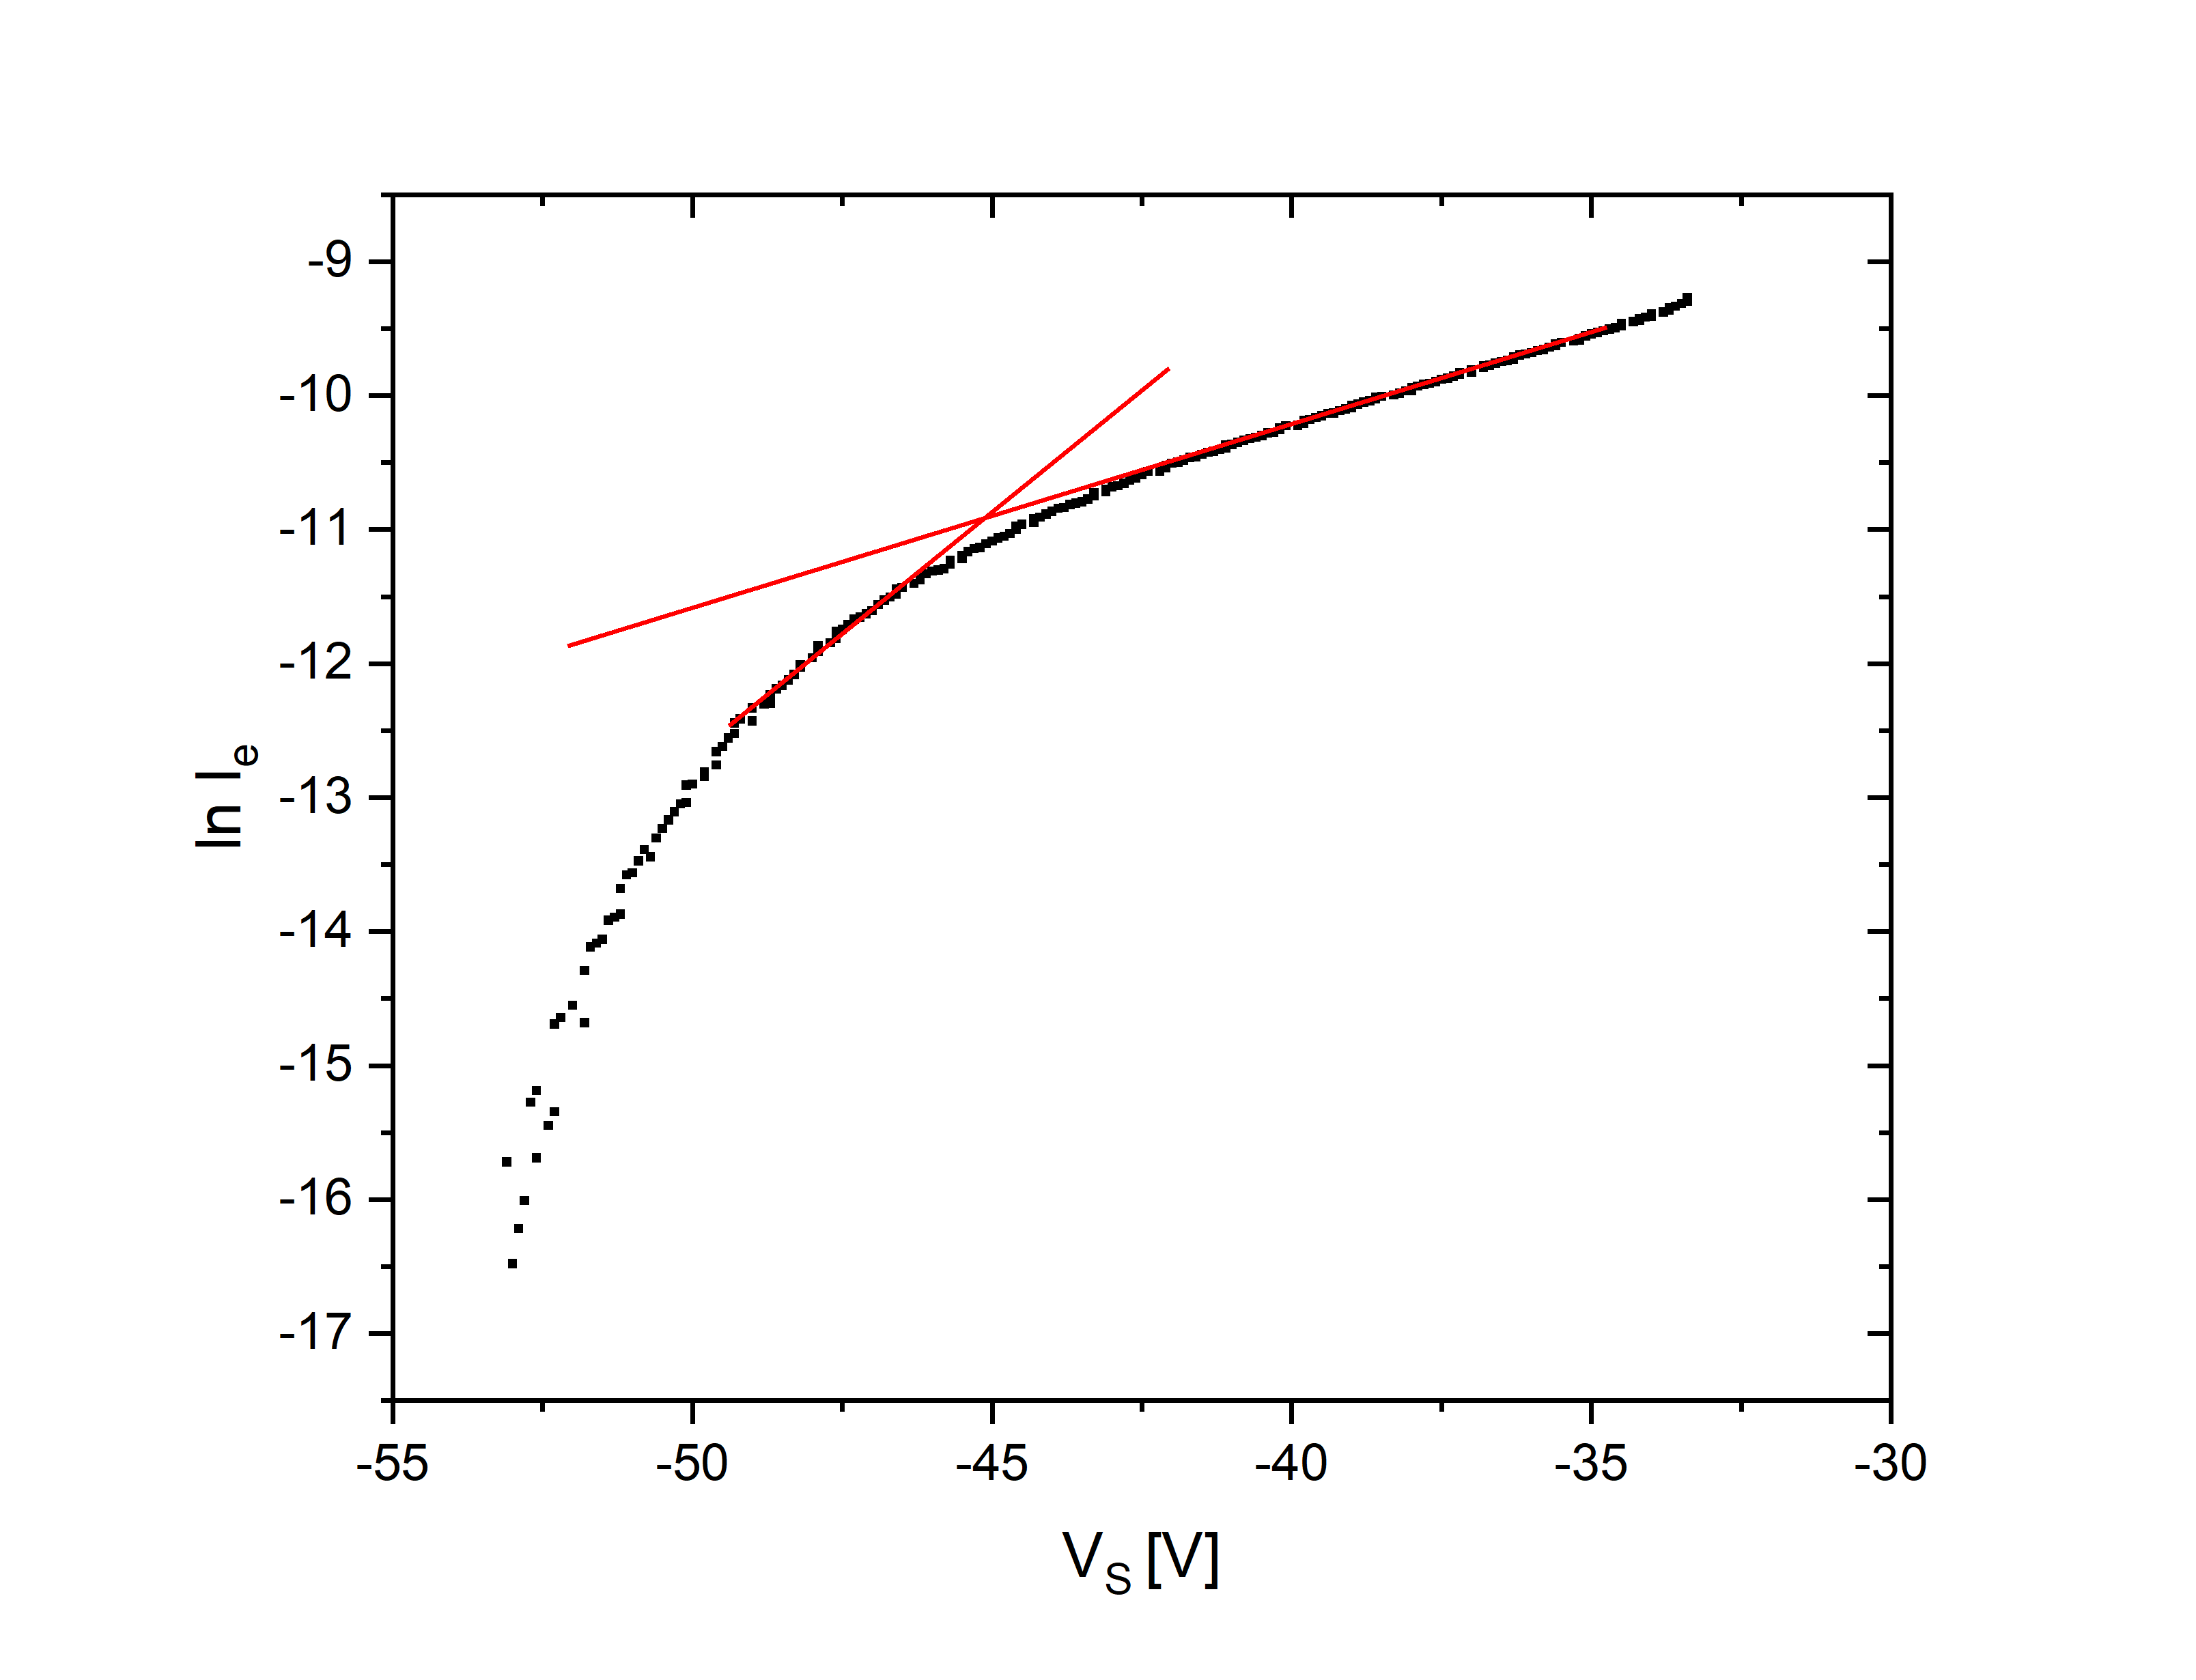
\includegraphics{data6Vp.png}}
		%\caption{$f(t) = 1/n$}
	\end{subfigure}
	\begin{subfigure}[b]{.49\textwidth}
		\centering
		\scalebox{.34}{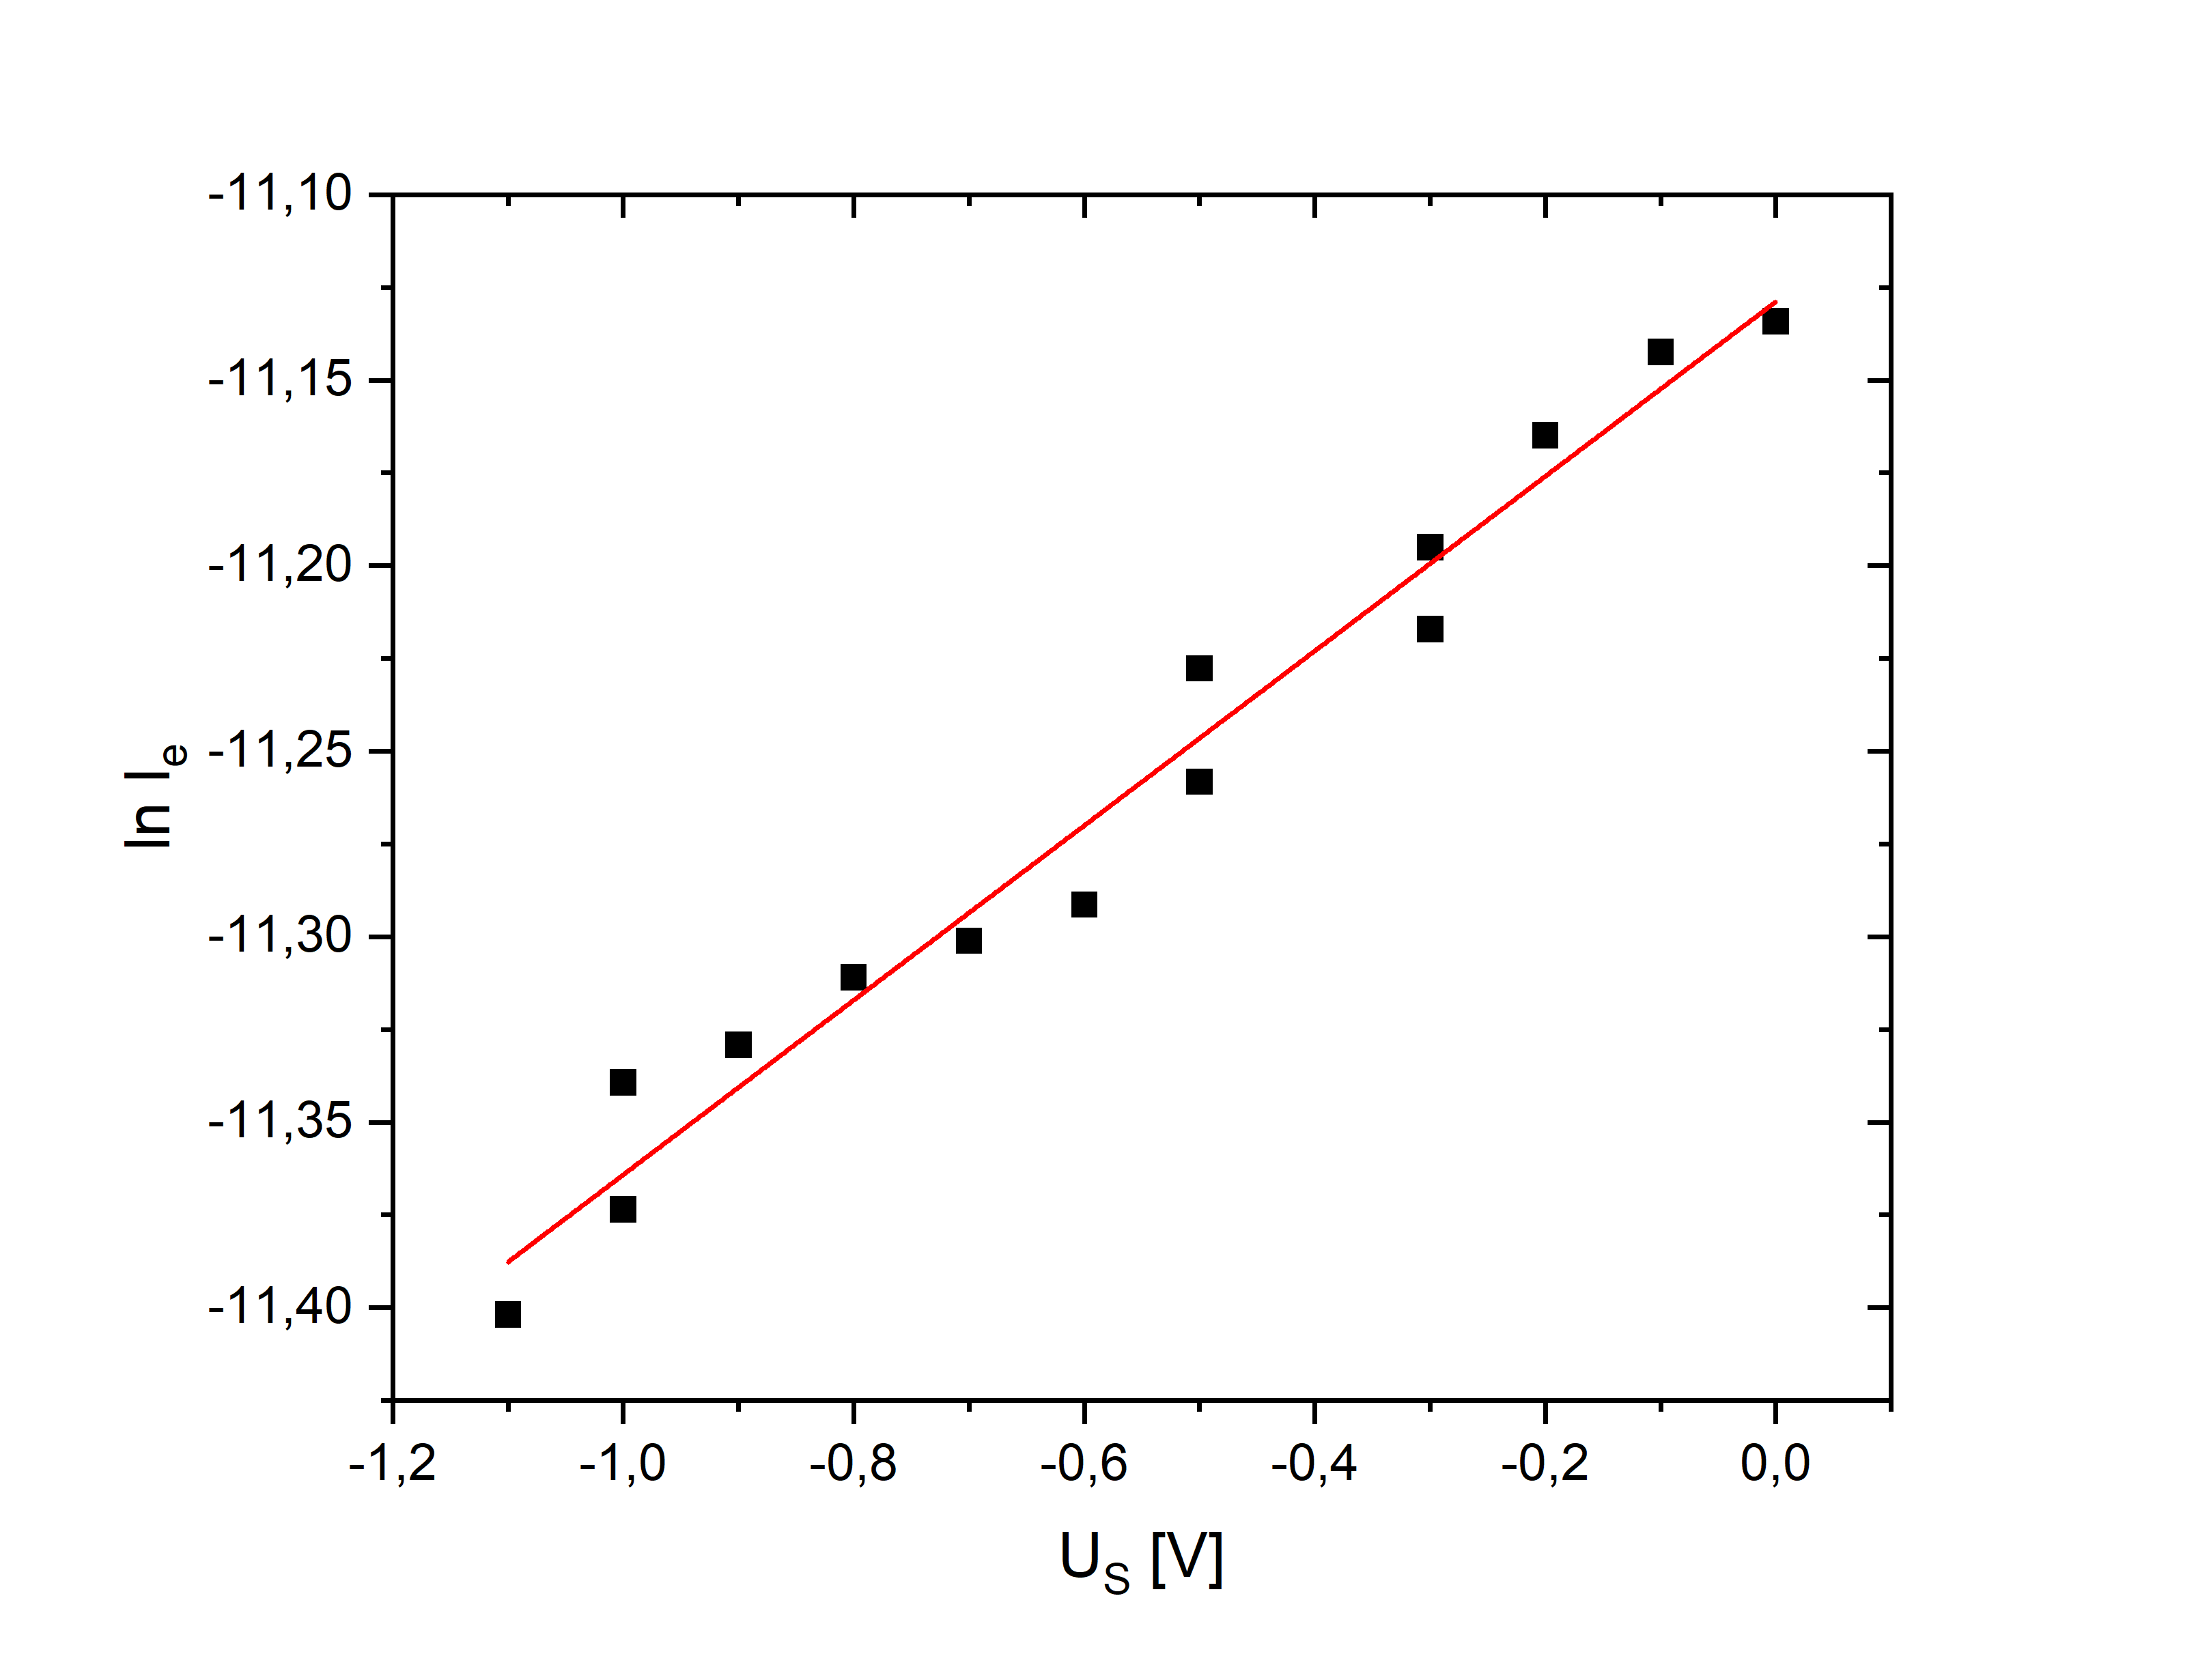
\includegraphics{data6T.png}}
		%\caption{$f(t) = \ln n$}
	\end{subfigure}
	\caption{Stanovení potenciálu plazmatu a elektronové teploty pomocí 
		průsečíku asymptot, $p = 16$ \si{\pascal} a $I_\text{v} = 40$ 
		\si{\milli\ampere}.}
	\label{data6}
\end{figure}

\begin{figure}[h!]
	\centering
	\begin{subfigure}[b]{.49\textwidth}
		\centering
		\scalebox{.34}{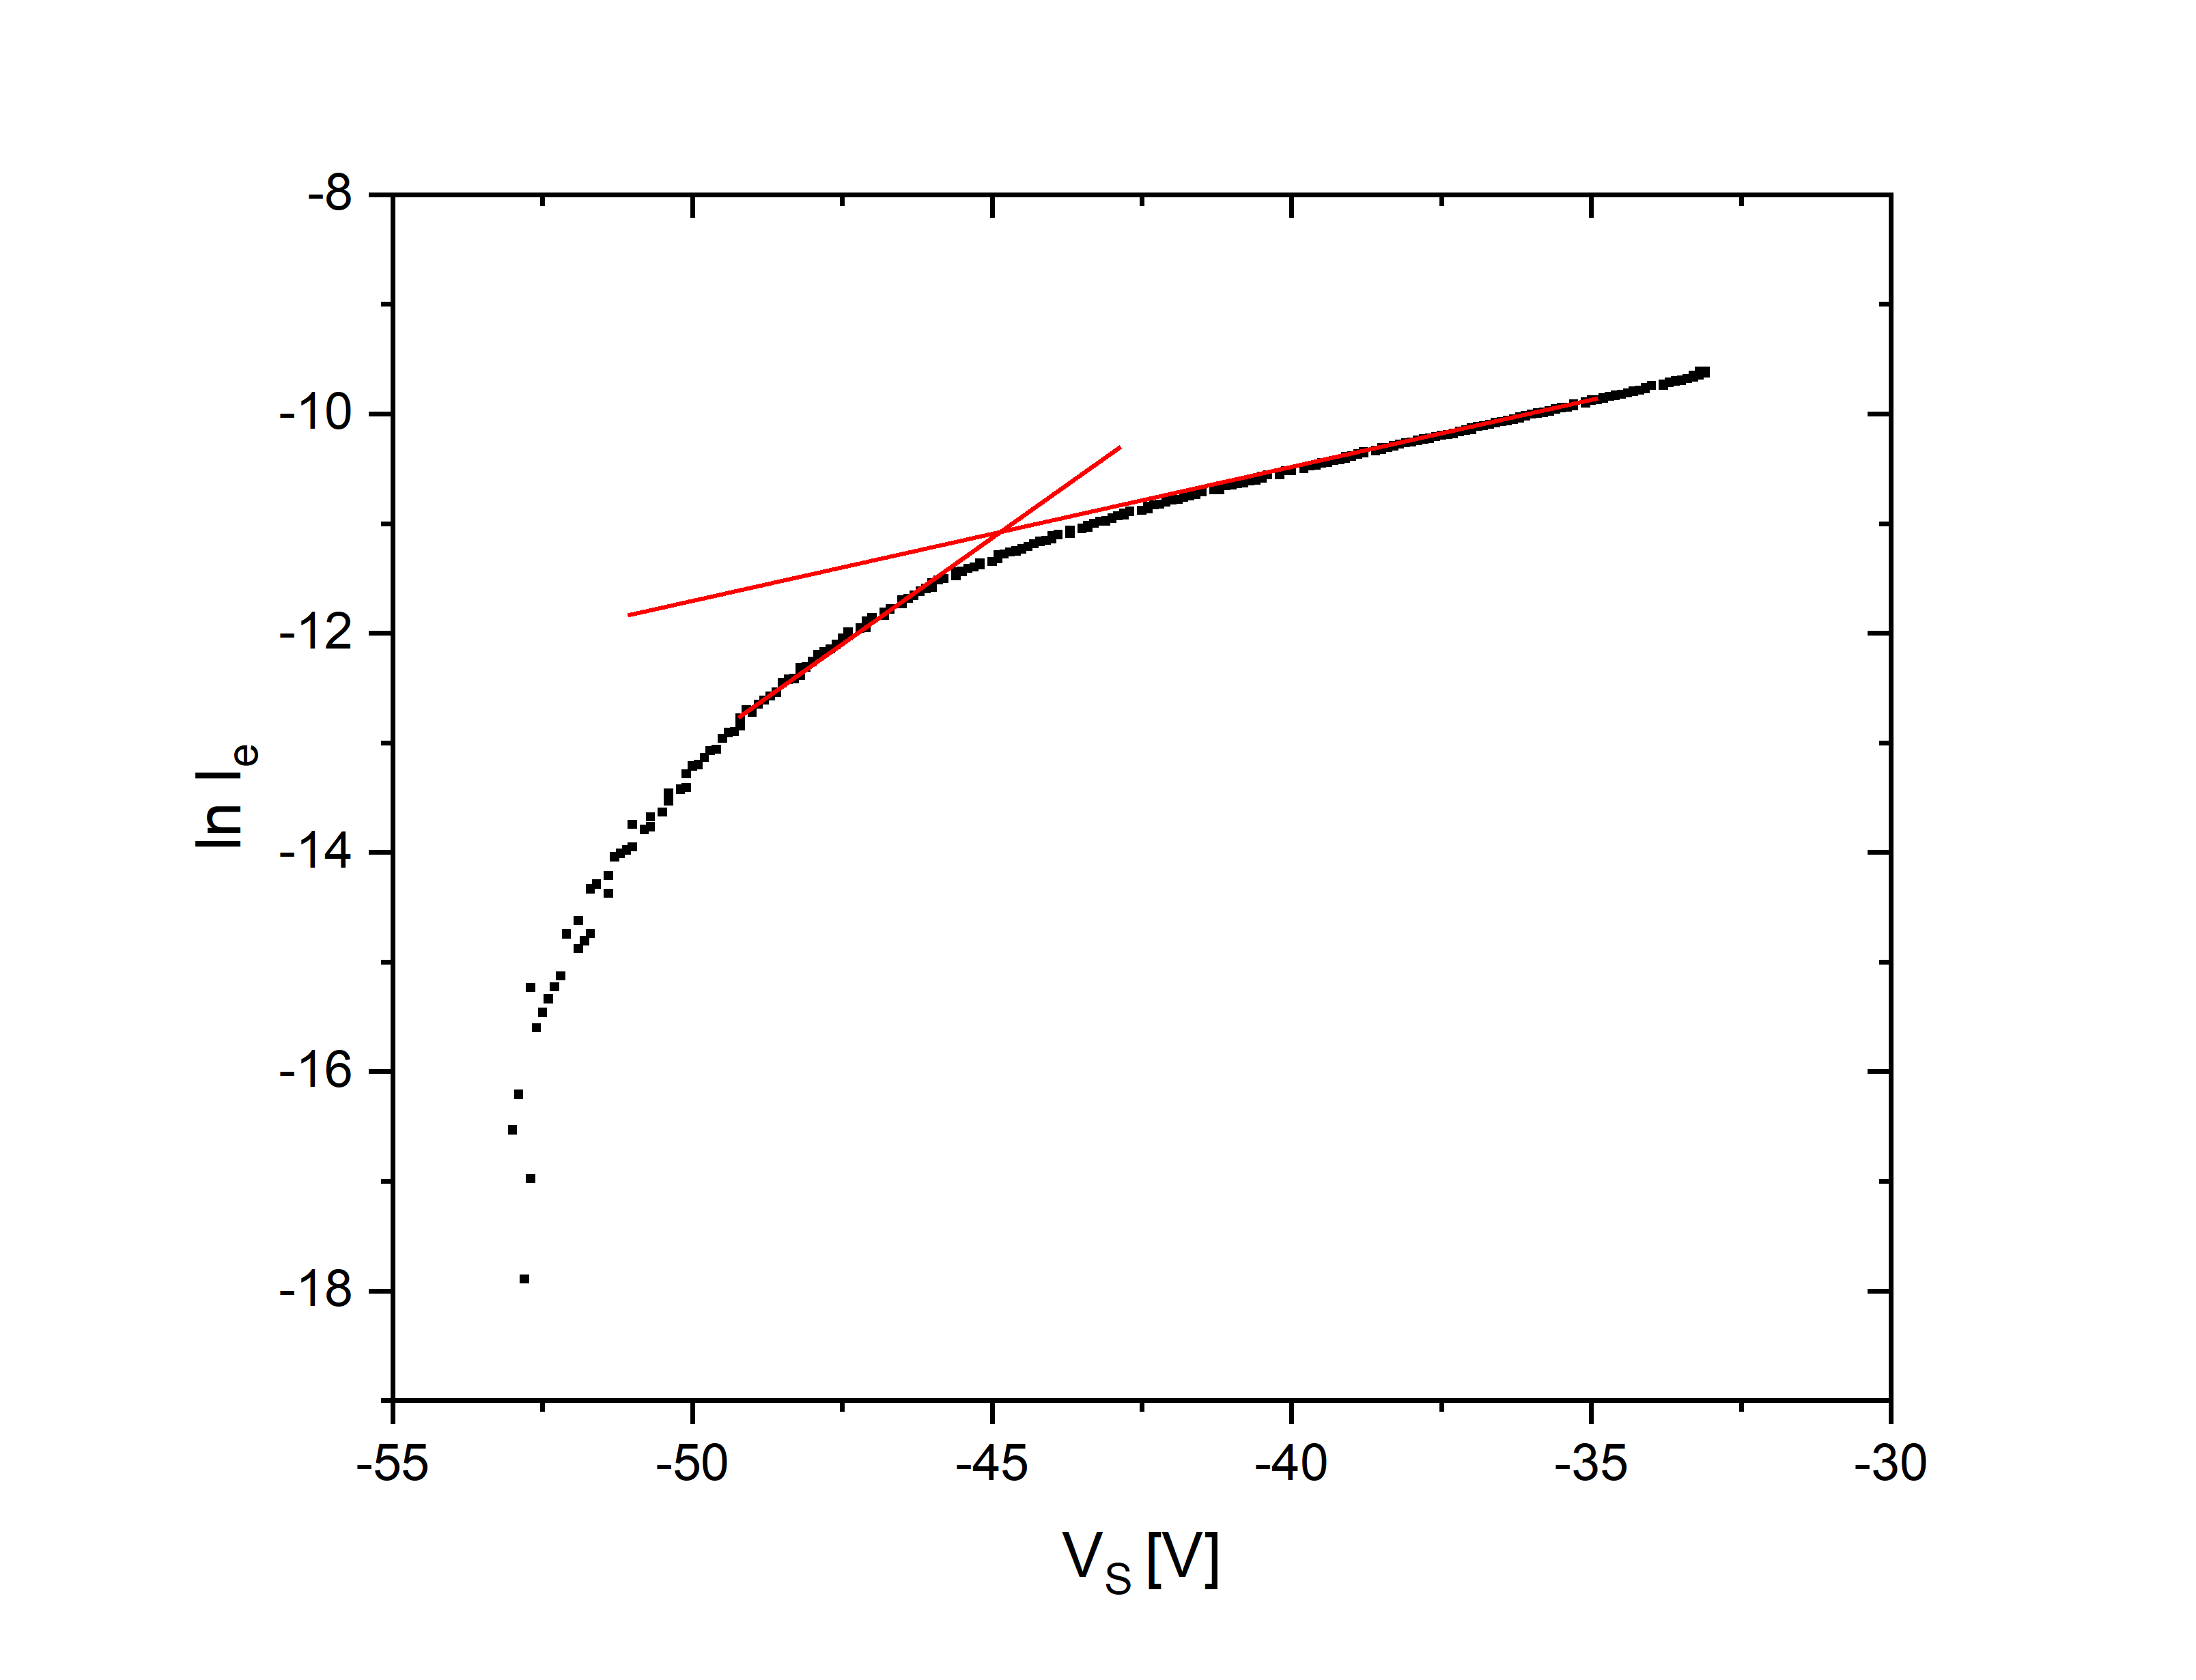
\includegraphics{data7Vp.png}}
		%\caption{$f(t) = 1/n$}
	\end{subfigure}
	\begin{subfigure}[b]{.49\textwidth}
		\centering
		\scalebox{.34}{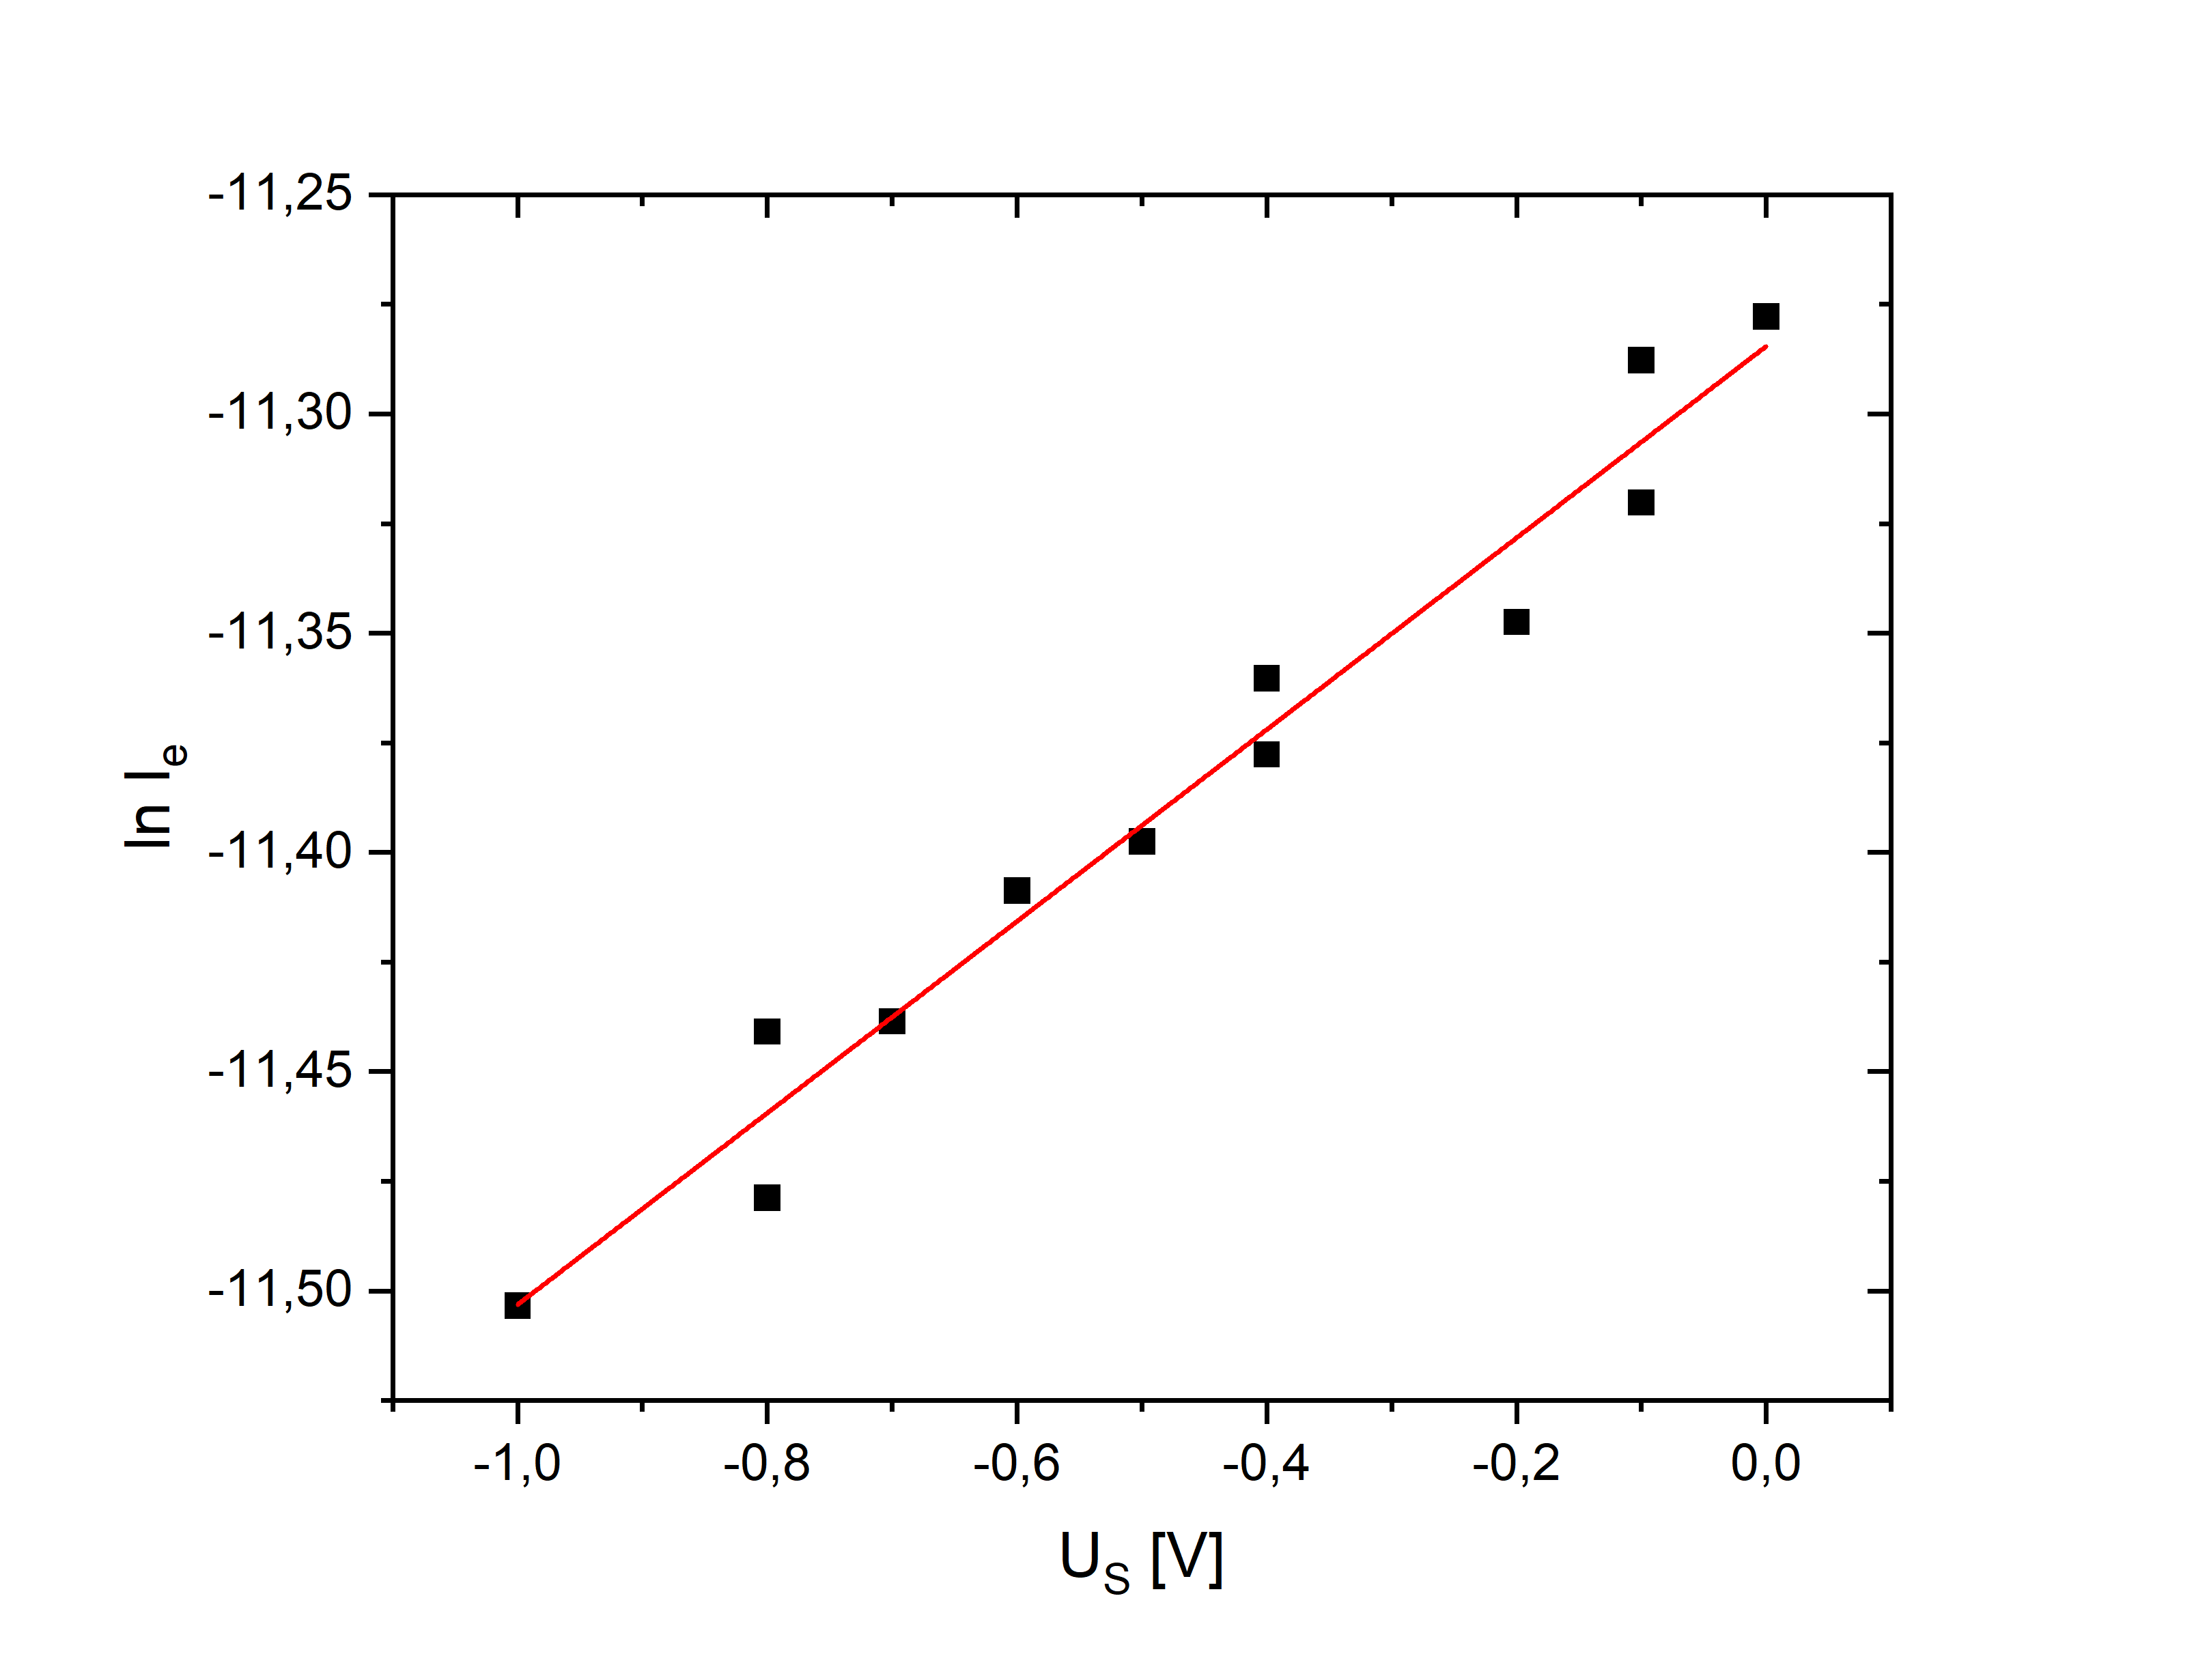
\includegraphics{data7T.png}}
		%\caption{$f(t) = \ln n$}
	\end{subfigure}
	\caption{Stanovení potenciálu plazmatu a elektronové teploty pomocí 
		průsečíku asymptot, $p = 8$ \si{\pascal} a $I_\text{v} = 40$ 
		\si{\milli\ampere}.}
	\label{data7}
\end{figure}



%%DRUHÁ DERIVACE PLOTY
\newpage
\begin{figure}[h]
	\centering
	\begin{subfigure}[b]{.49\textwidth}
		\centering
		\scalebox{.34}{\includegraphics{graph2.png}}
		%\caption{$f(t) = 1/n$}
	\end{subfigure}
	\begin{subfigure}[b]{.49\textwidth}
		\centering
		\scalebox{.34}{\includegraphics{graph25.png}}
		%\caption{$f(t) = \ln n$}
	\end{subfigure}
	\caption{Stanovení potenciálu plazmatu a elektronové teploty pomocí druhé 
	derivace, $p = 160$ 
	\si{\pascal} a $I_\text{v} = 30$ \si{\milli\ampere}, $V_{p,d} = 
	-43,4$ V.}
	\label{data1sec}
\end{figure}

\begin{figure}[h]
	\centering
	\begin{subfigure}[b]{.49\textwidth}
		\centering
		\scalebox{.34}{\includegraphics{graph4.png}}
		%\caption{$f(t) = 1/n$}
	\end{subfigure}
	\begin{subfigure}[b]{.49\textwidth}
		\centering
		\scalebox{.34}{\includegraphics{graph26.png}}
		%\caption{$f(t) = \ln n$}
	\end{subfigure}
	\caption{Stanovení potenciálu plazmatu a elektronové teploty pomocí druhé 
	derivace, $p = 160$ 
	\si{\pascal} a 
		$I_\text{v} = 40$ \si{\milli\ampere}, $V_{p,d} = -39,7$ V.}
	\label{data0sec}
\end{figure}

\newpage
\begin{figure}[h]
	\centering
	\begin{subfigure}[b]{.49\textwidth}
		\centering
		\scalebox{.34}{\includegraphics{graph6.png}}
		%\caption{$f(t) = 1/n$}
	\end{subfigure}
	\begin{subfigure}[b]{.49\textwidth}
		\centering
		\scalebox{.34}{\includegraphics{graph27.png}}
		%\caption{$f(t) = \ln n$}
	\end{subfigure}
	\caption{Stanovení potenciálu plazmatu a elektronové teploty pomocí druhé 
	derivace, $p = 160$ 
	\si{\pascal} a $I_\text{v} = 50$ \si{\milli\ampere}, $V_{p,d} = 
	-37,5$ V.}
	\label{data2sec}
\end{figure}



\begin{figure}[h]
	\centering
	\begin{subfigure}[b]{.49\textwidth}
		\centering
		\scalebox{.34}{\includegraphics{graph8.png}}
		%\caption{$f(t) = 1/n$}
	\end{subfigure}
	\begin{subfigure}[b]{.49\textwidth}
		\centering
		\scalebox{.34}{\includegraphics{graph28.png}}
		%\caption{$f(t) = \ln n$}
	\end{subfigure}
	\caption{Stanovení potenciálu plazmatu a elektronové teploty pomocí druhé 
	derivace, $p = 320$ 
	\si{\pascal} a $I_\text{v} = 40$ \si{\milli\ampere}, $V_{p,d} = 
	-45,8$ V.}
	\label{data3sec}
\end{figure}

\newpage
\begin{figure}[h]
	\centering
	\begin{subfigure}[b]{.49\textwidth}
		\centering
		\scalebox{.34}{\includegraphics{graph10.png}}
		%\caption{$f(t) = 1/n$}
	\end{subfigure}
	\begin{subfigure}[b]{.49\textwidth}
		\centering
		\scalebox{.34}{\includegraphics{graph29.png}}
		%\caption{$f(t) = \ln n$}
	\end{subfigure}
	\caption{Stanovení potenciálu plazmatu a elektronové teploty pomocí druhé 
	derivace, $p = 80$ 
	\si{\pascal} a $I_\text{v} = 40$ \si{\milli\ampere}, $V_{p,d} = 
	-42,8$ V.}
	\label{data4sec}
\end{figure}

\begin{figure}[h]
	\centering
	\begin{subfigure}[b]{.49\textwidth}
		\centering
		\scalebox{.34}{\includegraphics{graph12.png}}
		%\caption{$f(t) = 1/n$}
	\end{subfigure}
	\begin{subfigure}[b]{.49\textwidth}
		\centering
		\scalebox{.34}{\includegraphics{graph30.png}}
		%\caption{$f(t) = \ln n$}
	\end{subfigure}
	\caption{Stanovení potenciálu plazmatu a elektronové teploty pomocí druhé 
	derivace, $p = 32$ 
	\si{\pascal} a $I_\text{v} = 40$ \si{\milli\ampere}, $V_{p,d} = 
	-43,4$ V.}
	\label{data5sec}
\end{figure}

\newpage
\begin{figure}[h!]
	\centering
	\begin{subfigure}[b]{.49\textwidth}
		\centering
		\scalebox{.34}{\includegraphics{graph14.png}}
		%\caption{$f(t) = 1/n$}
	\end{subfigure}
	\begin{subfigure}[b]{.49\textwidth}
		\centering
		\scalebox{.34}{\includegraphics{graph31.png}}
		%\caption{$f(t) = \ln n$}
	\end{subfigure}
	\caption{Stanovení potenciálu plazmatu a elektronové teploty pomocí druhé 
	derivace, $p = 16$ 
	\si{\pascal} a $I_\text{v} = 40$ \si{\milli\ampere}, $V_{p,d} = 
	-44,4$ V.}
	\label{data6sec}
\end{figure}

\begin{figure}[h!]
	\centering
	\begin{subfigure}[b]{.49\textwidth}
		\centering
		\scalebox{.34}{\includegraphics{graph16.png}}
		%\caption{$f(t) = 1/n$}
	\end{subfigure}
	\begin{subfigure}[b]{.49\textwidth}
		\centering
		\scalebox{.34}{\includegraphics{graph32.png}}
		%\caption{$f(t) = \ln n$}
	\end{subfigure}
	\caption{Stanovení potenciálu plazmatu a elektronové teploty pomocí druhé 
	derivace, $p = 8$ 
	\si{\pascal} a $I_\text{v} = 40$ \si{\milli\ampere}, $V_{p,d} = 
	-43,8$ \si{\volt}.}
	\label{data7sec}
\end{figure}

\clearpage
\subsection{Rozdělovací funkce energií}
Voltampérovou charakteristiku bez a s poruchovým napětím měříme současně tak, 
že periodicky připojujeme a odpojujeme poruchové napětí, viz 
obr.~\ref{demonstracni}, přičemž chybějící 
hodnoty získáme pomocí polynomického fitu. Z charakteristiky bez 
poruchového napětí určíme plovoucí a plazmový potenciál podobně jako v 
předchozí části metodou druhé derivace, viz tab. \ref{tab3}. Po odečtení 
iontového proudu jsou VA 
charakteristiky za dvou různých tlaků a~výbojových proudů vyneseny do 
obr.~\ref{Ieporucha}. Proud $\Delta i$ je určen z rozdílu dané dvojice 
křivek. 
Závislost $f(\vert U_s\vert) = \sqrt{\vert U_s\vert}\Delta i$ je vynesena do 
obr.~\ref{rozdeleniG1}--\ref{rozdeleniG3}. Dle rovnice~\eqref{eq:rozdeleni} 
jsou naměřené hodnoty proloženy Maxwellovým, Druyvesteynovým a rozdělením s 
proměnným parametrem $K$. 
Pozorujeme, že Druyvesteynovo rozdělení odpovídá našim datům více než 
Maxwellovo. Parametr $B$ v rovnici \eqref{eq:rozdeleni} je roven součinu $kT$. 
Lze z něj tedy určit teplotu elektronů $T\approx7$\,eV, ta je v porovnání s 
teplotou určenou v předchozí části (tabulka \ref{tab2}) dvojnásobná. Pro 
určení rozdělovací funkce jsme použili také metodu druhé derivace dle rovnice 
\eqref{delta i}, viz obr.~\ref{rozdeleniD2G1}--\ref{rozdeleniD2G3}. Tato metoda 
vychází pouze pro obr.~\ref{rozdeleniD2G2}, u ostatních grafů je nepřesná, a 
proto jsme ji k dalšímu vyhodnocení nepoužili.


\begin{center}
	\begin{table}[h!]
		\centering
		\caption{Plovoucí a plazmové potenciály bez přiloženého poruchového 
		napětí, parametry $K$ a teplota $T$.}
		\label{tab3}
		\begin{tabular}{|c|c|c|c|c|c|} \hline
			$p$ [\si{\pascal}] & $I_\text{v}$ [\si{\milli\ampere}] &  
			$V_\text{fl}$ [V] & 
			$V_\text{p}$ [V] & $K$ & $T$ [eV] \\ \hline
			80&55&-42,9&-39,9&3,38&6,83\\ \hline
			80&30&-47,3&-43,4&2,47&7,34\\ \hline
			16&55&-44,0&-42,8&2,71&6,54\\ \hline
			
		\end{tabular}
	\end{table}
\end{center}

\begin{figure}[h!]
	\centering
	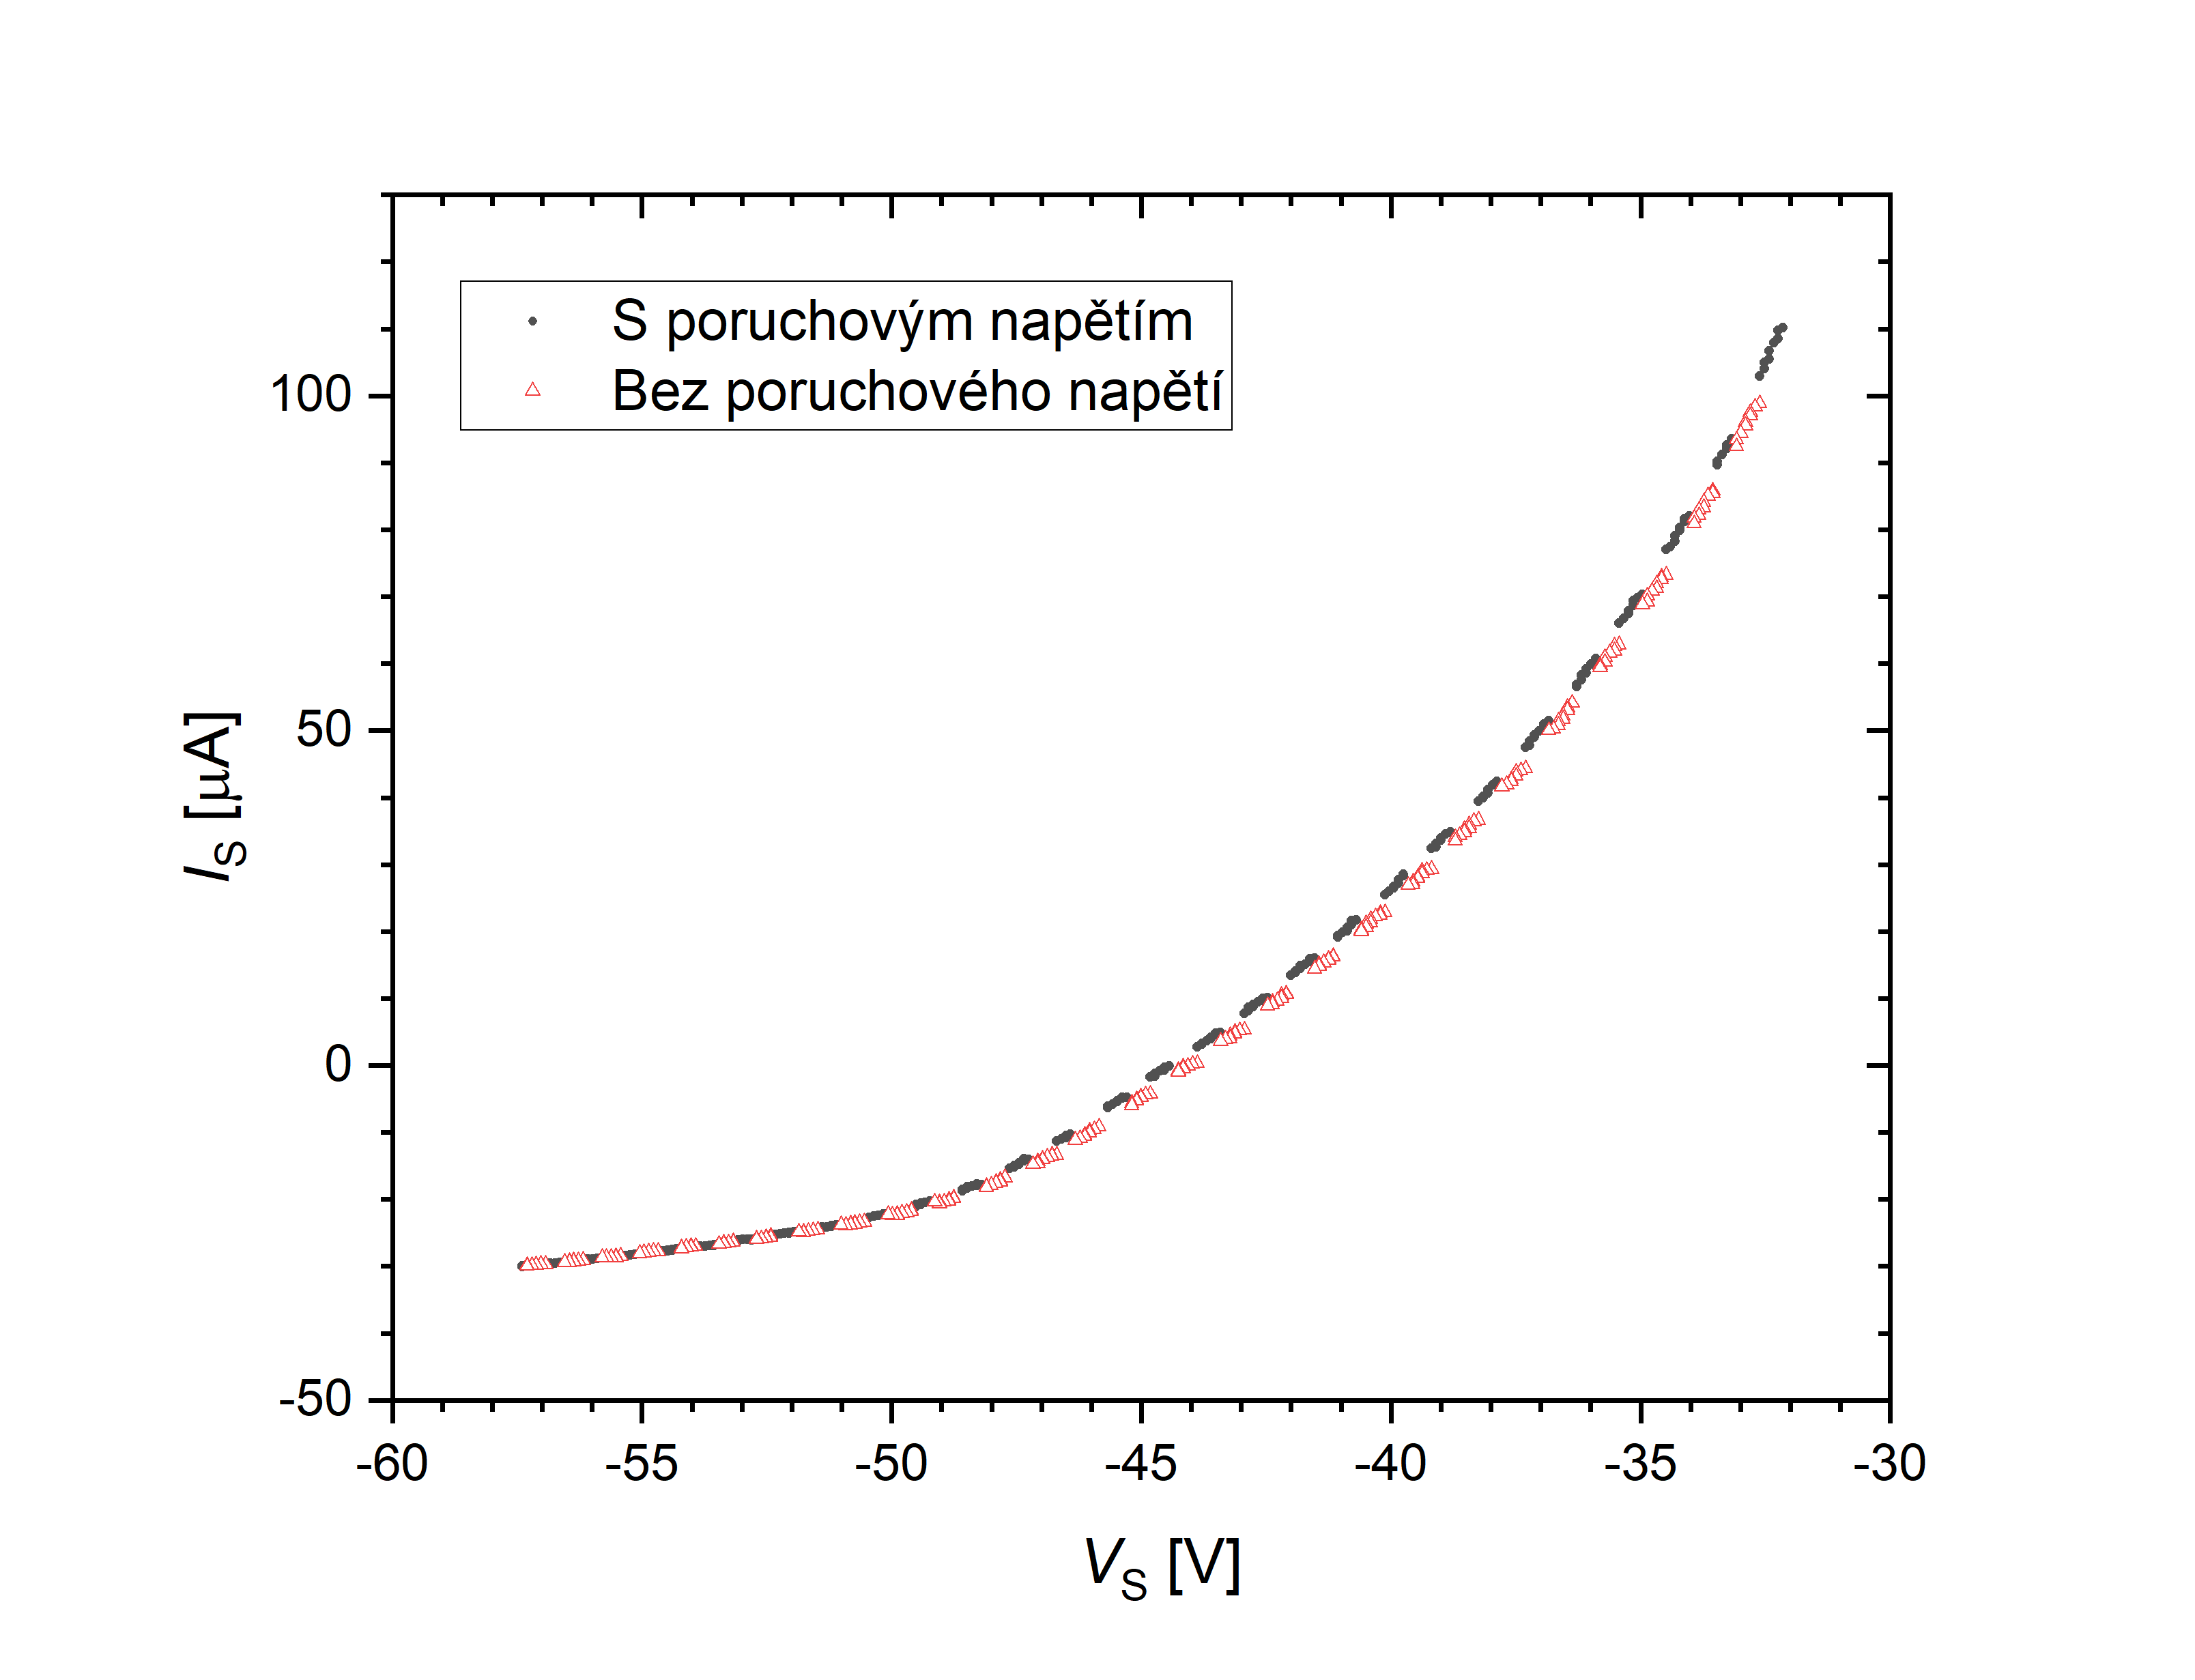
\includegraphics[width=135mm]{demonstracni.png}
	\caption{VA charakteristika s poruchovým a 
		bez poruchového napětí, $p=16$\,\si{\pascal}, 
		$I_v~=~55$\,\si{\milli\ampere}.}
	\label{demonstracni}
\end{figure}

\begin{figure}[h!]
	\centering
	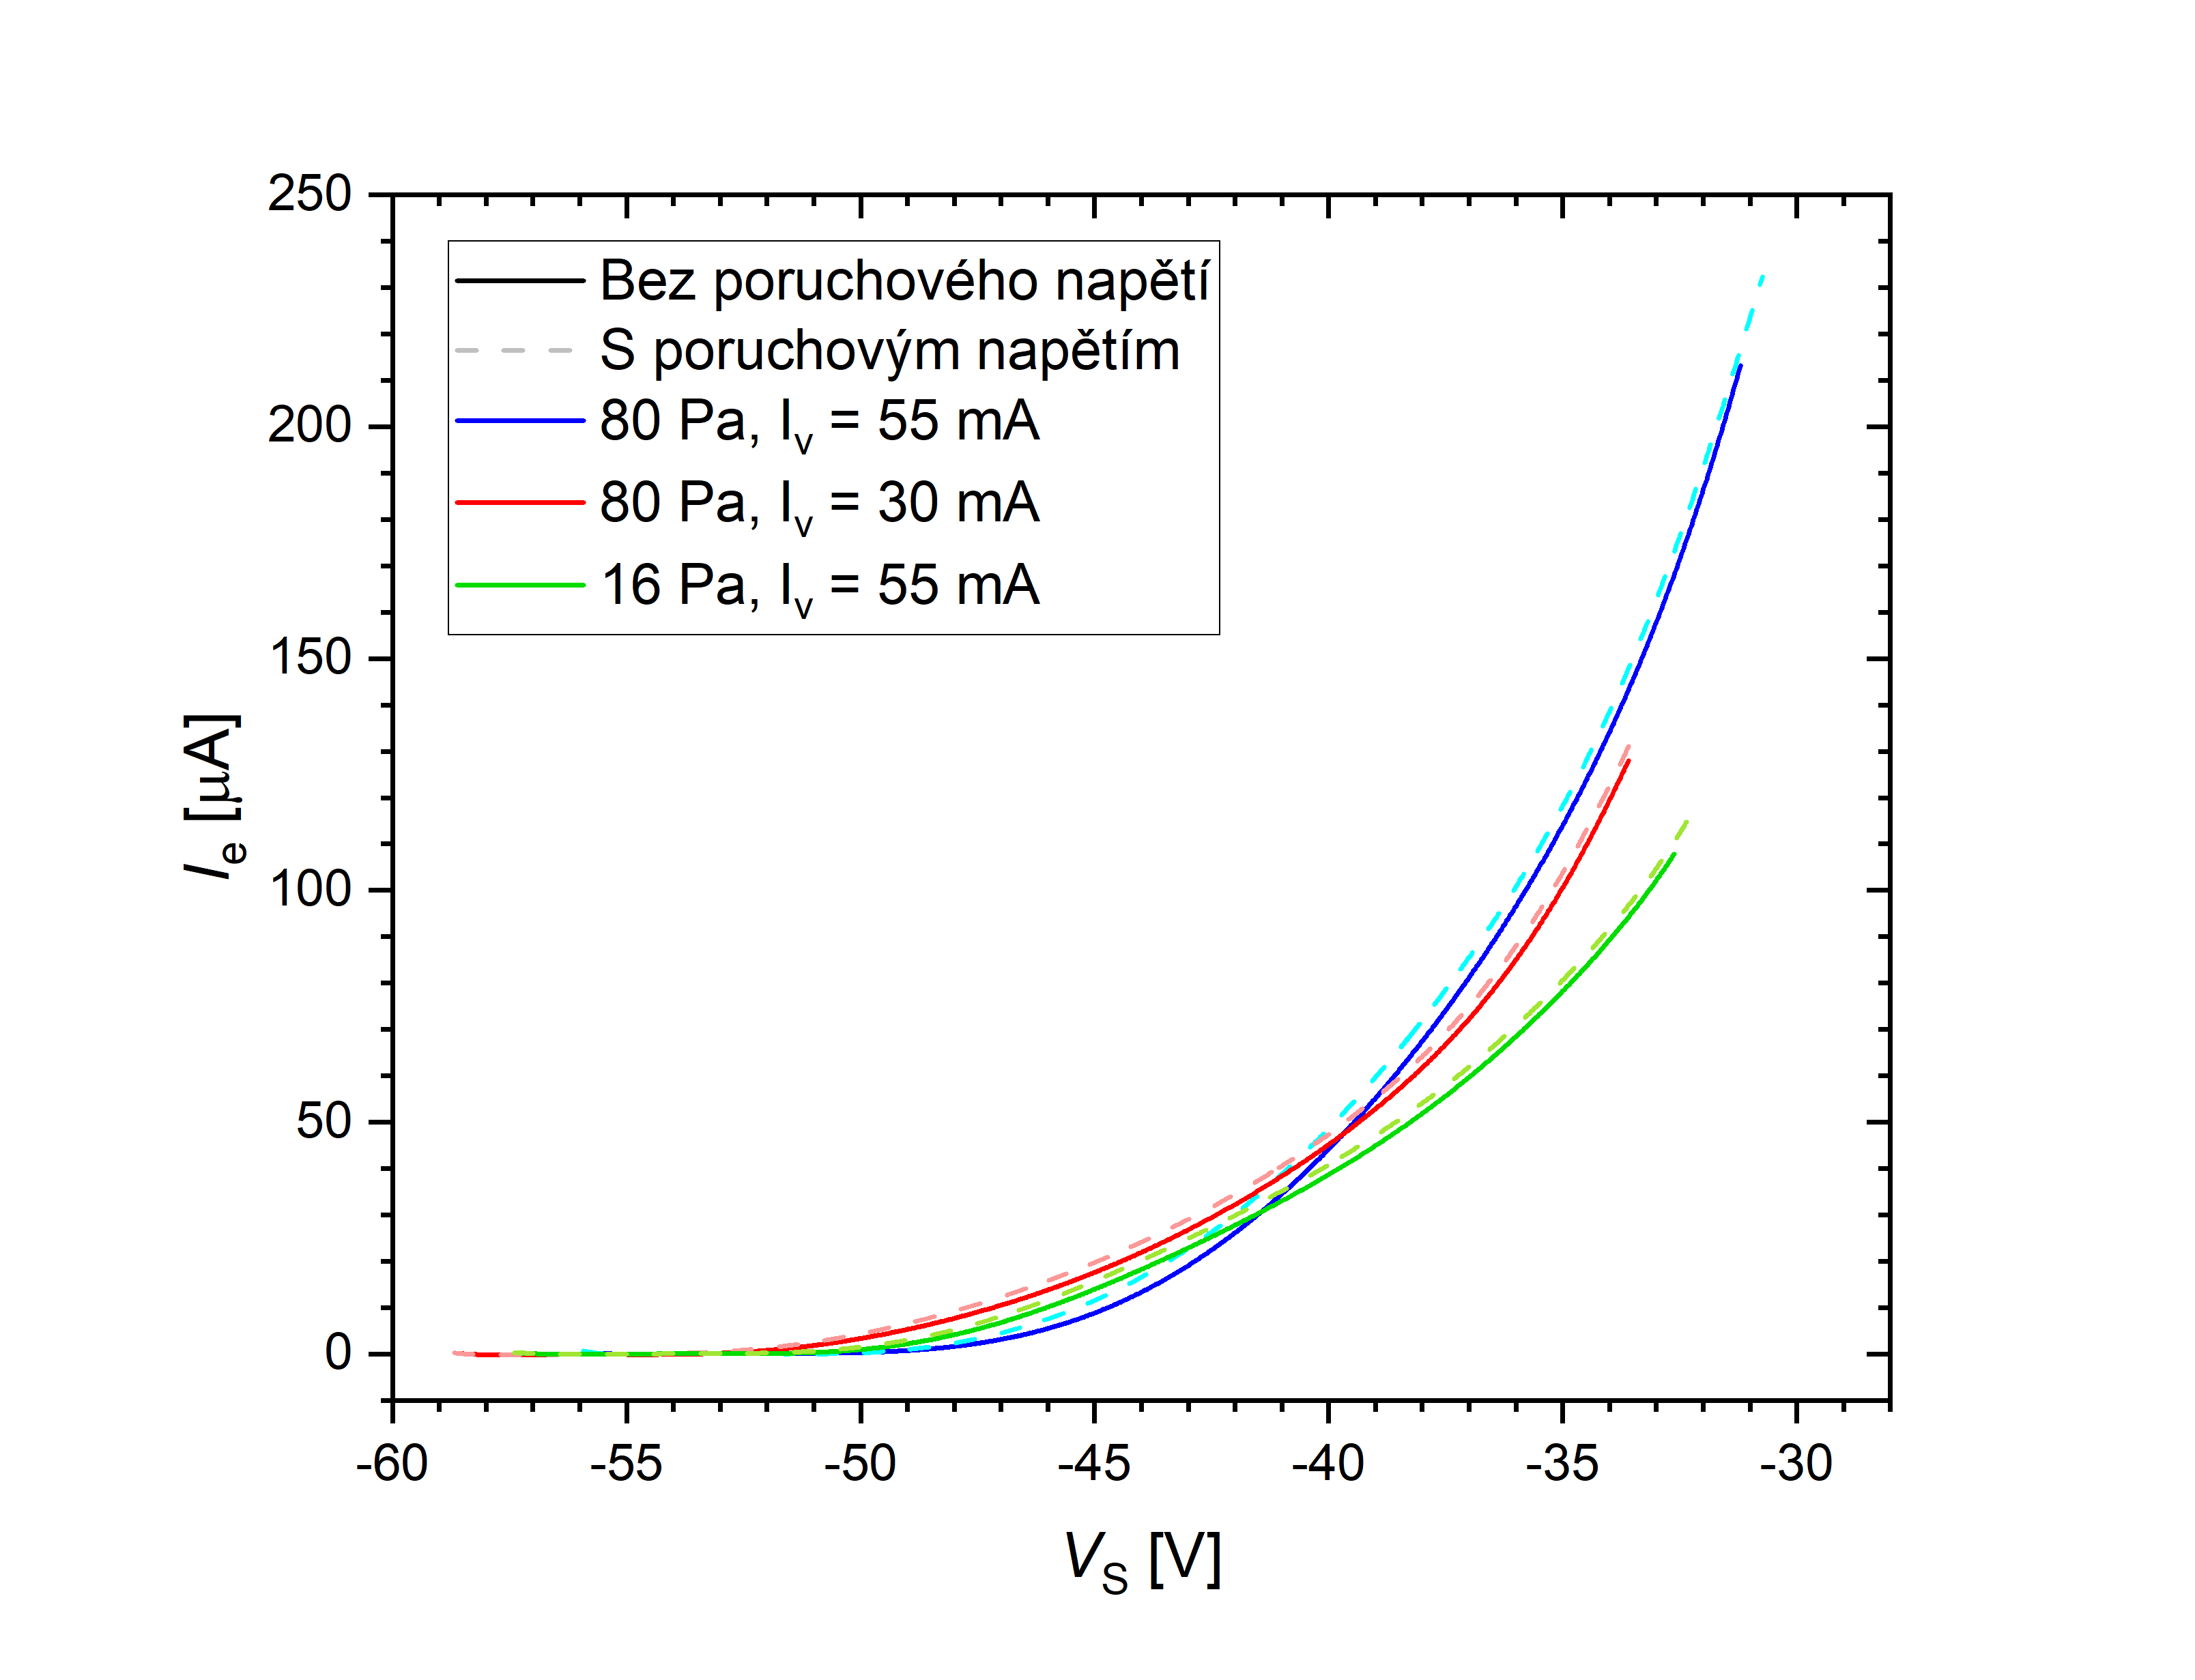
\includegraphics[width=135mm]{Ieporucha.png}
	\caption{VA charakteristiky s odečteným iontovým proudem, s poruchovým a 
	bez poruchového napětí.}
	\label{Ieporucha}
\end{figure}

\begin{figure}[h!]
	\centering
	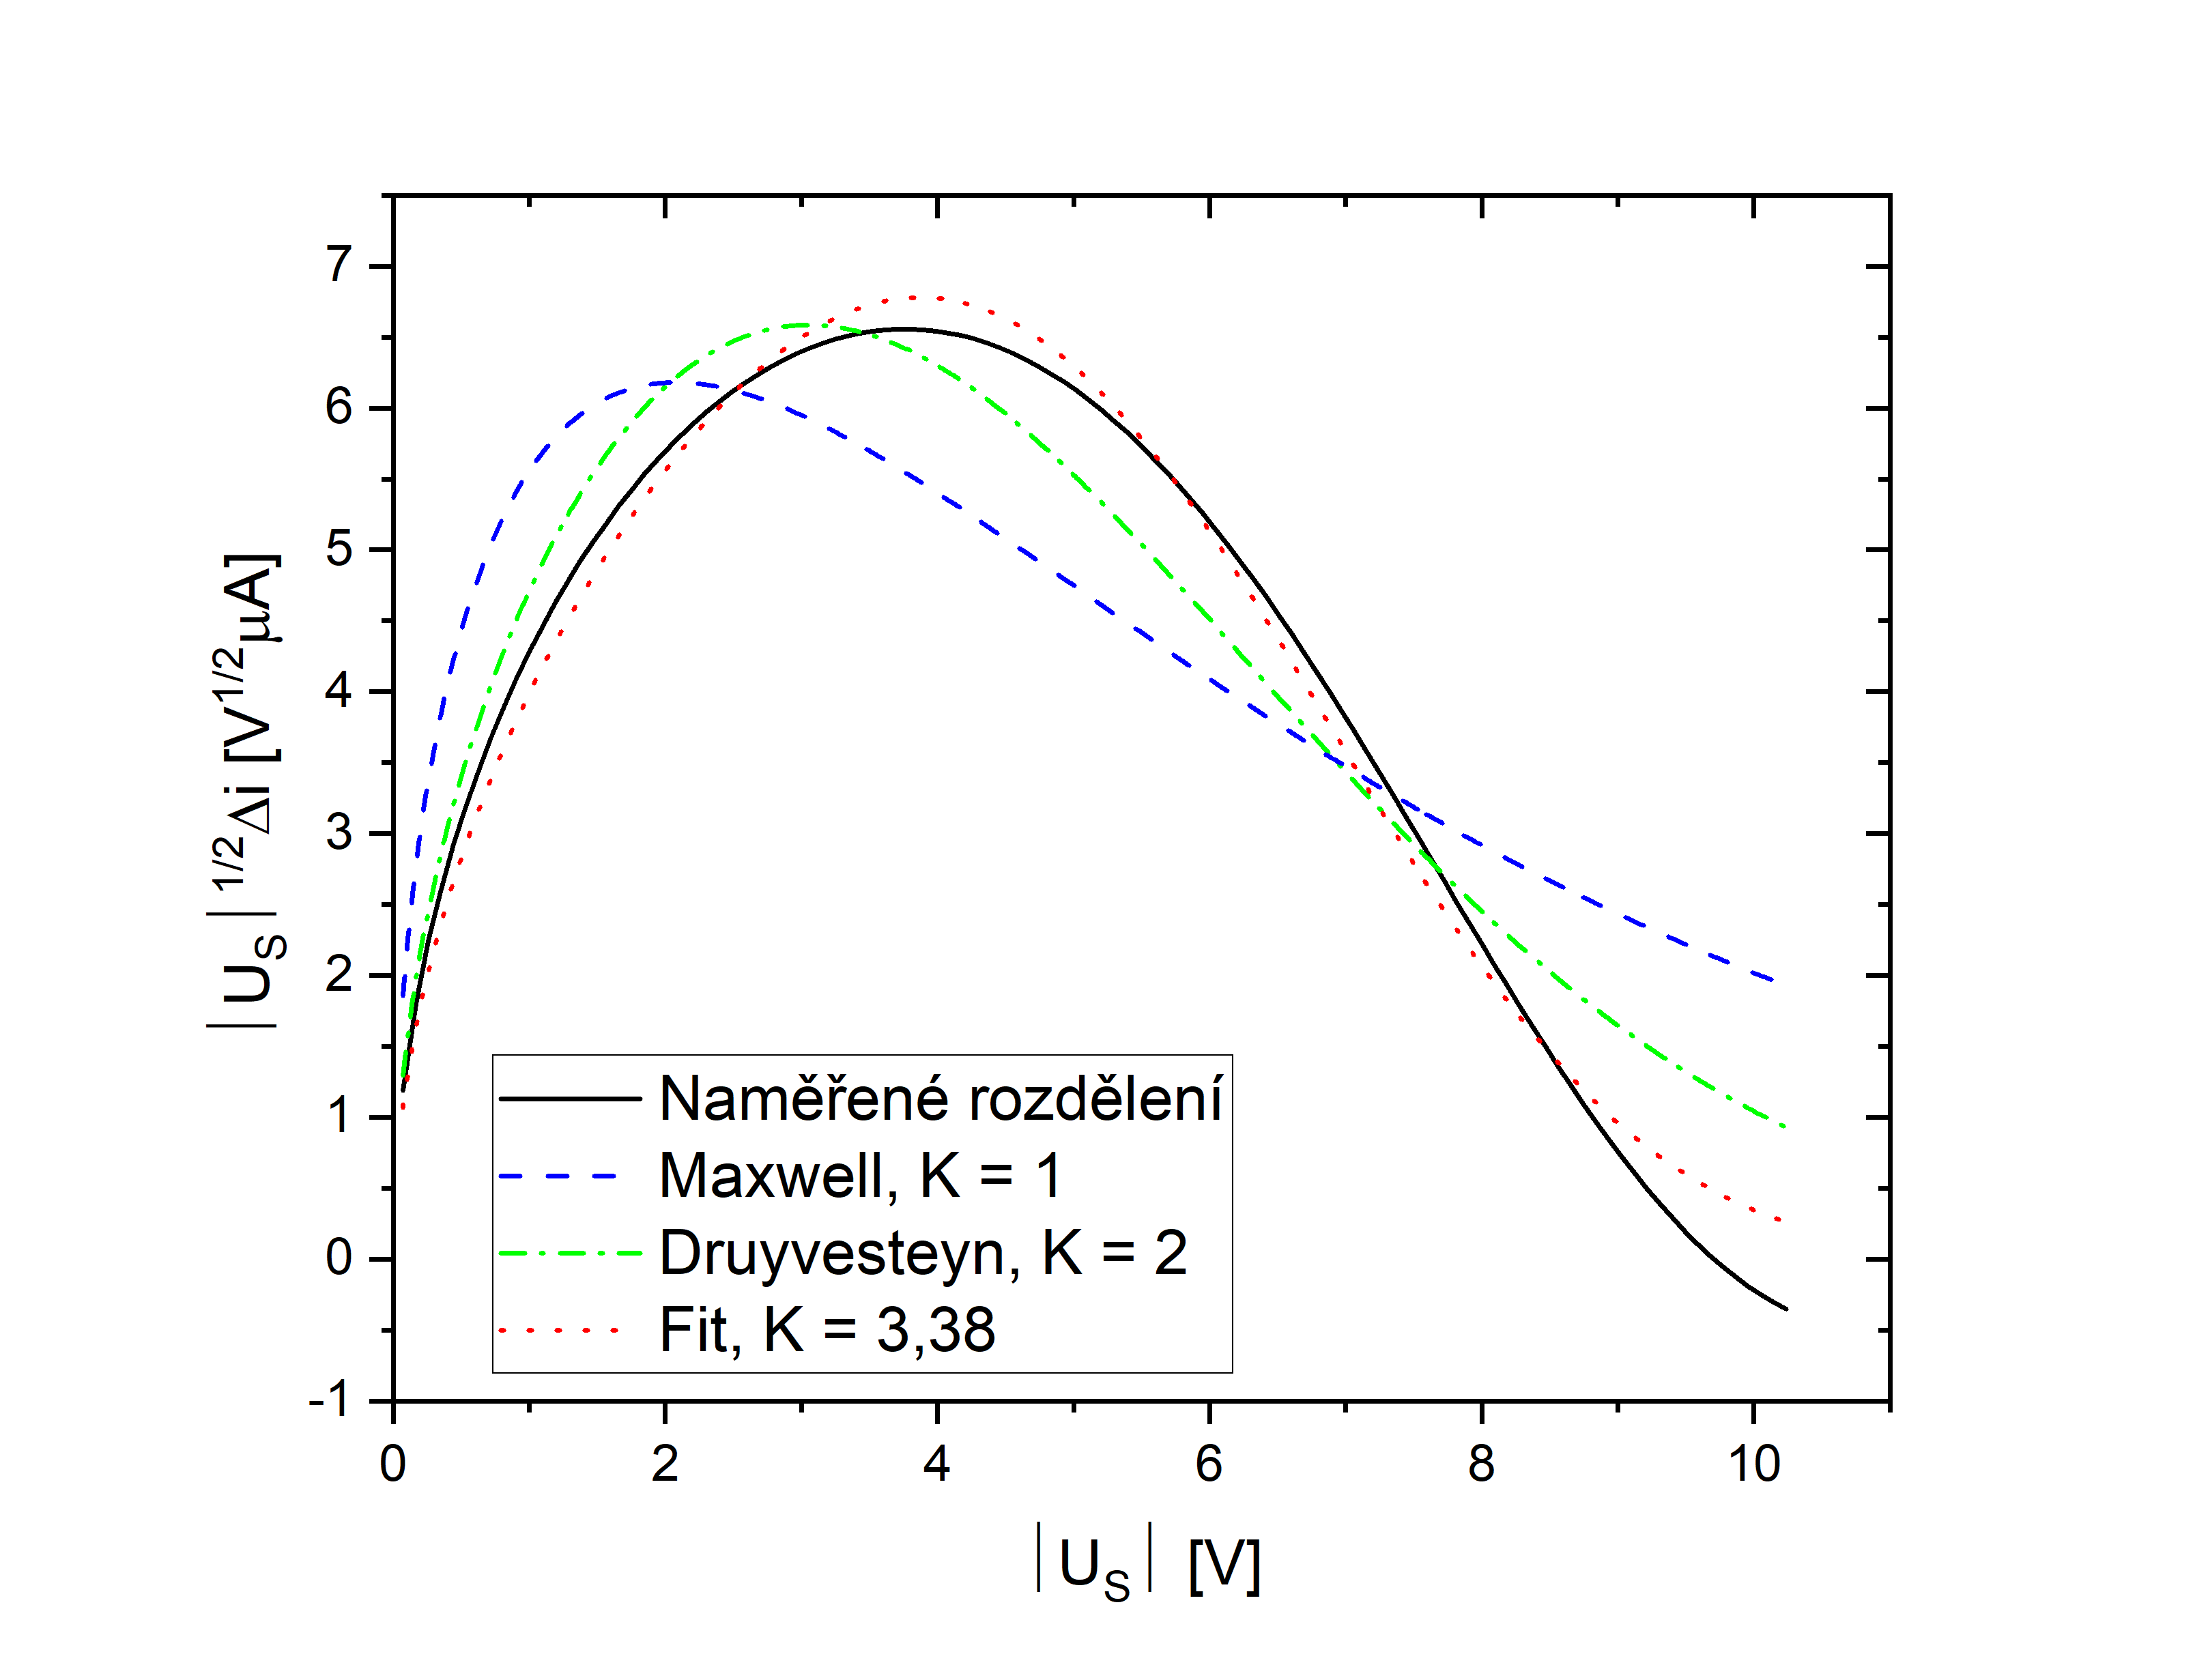
\includegraphics[width=135mm]{rozdeleniG1.png}
	\caption{Rozdělovací funkce určena metodou poruchového napětí, 
	$p=80$\,\si{\pascal}, $I_v = 55$\,\si{\milli\ampere}.}
	\label{rozdeleniG1}
\end{figure}

\begin{figure}[h!]
	\centering
	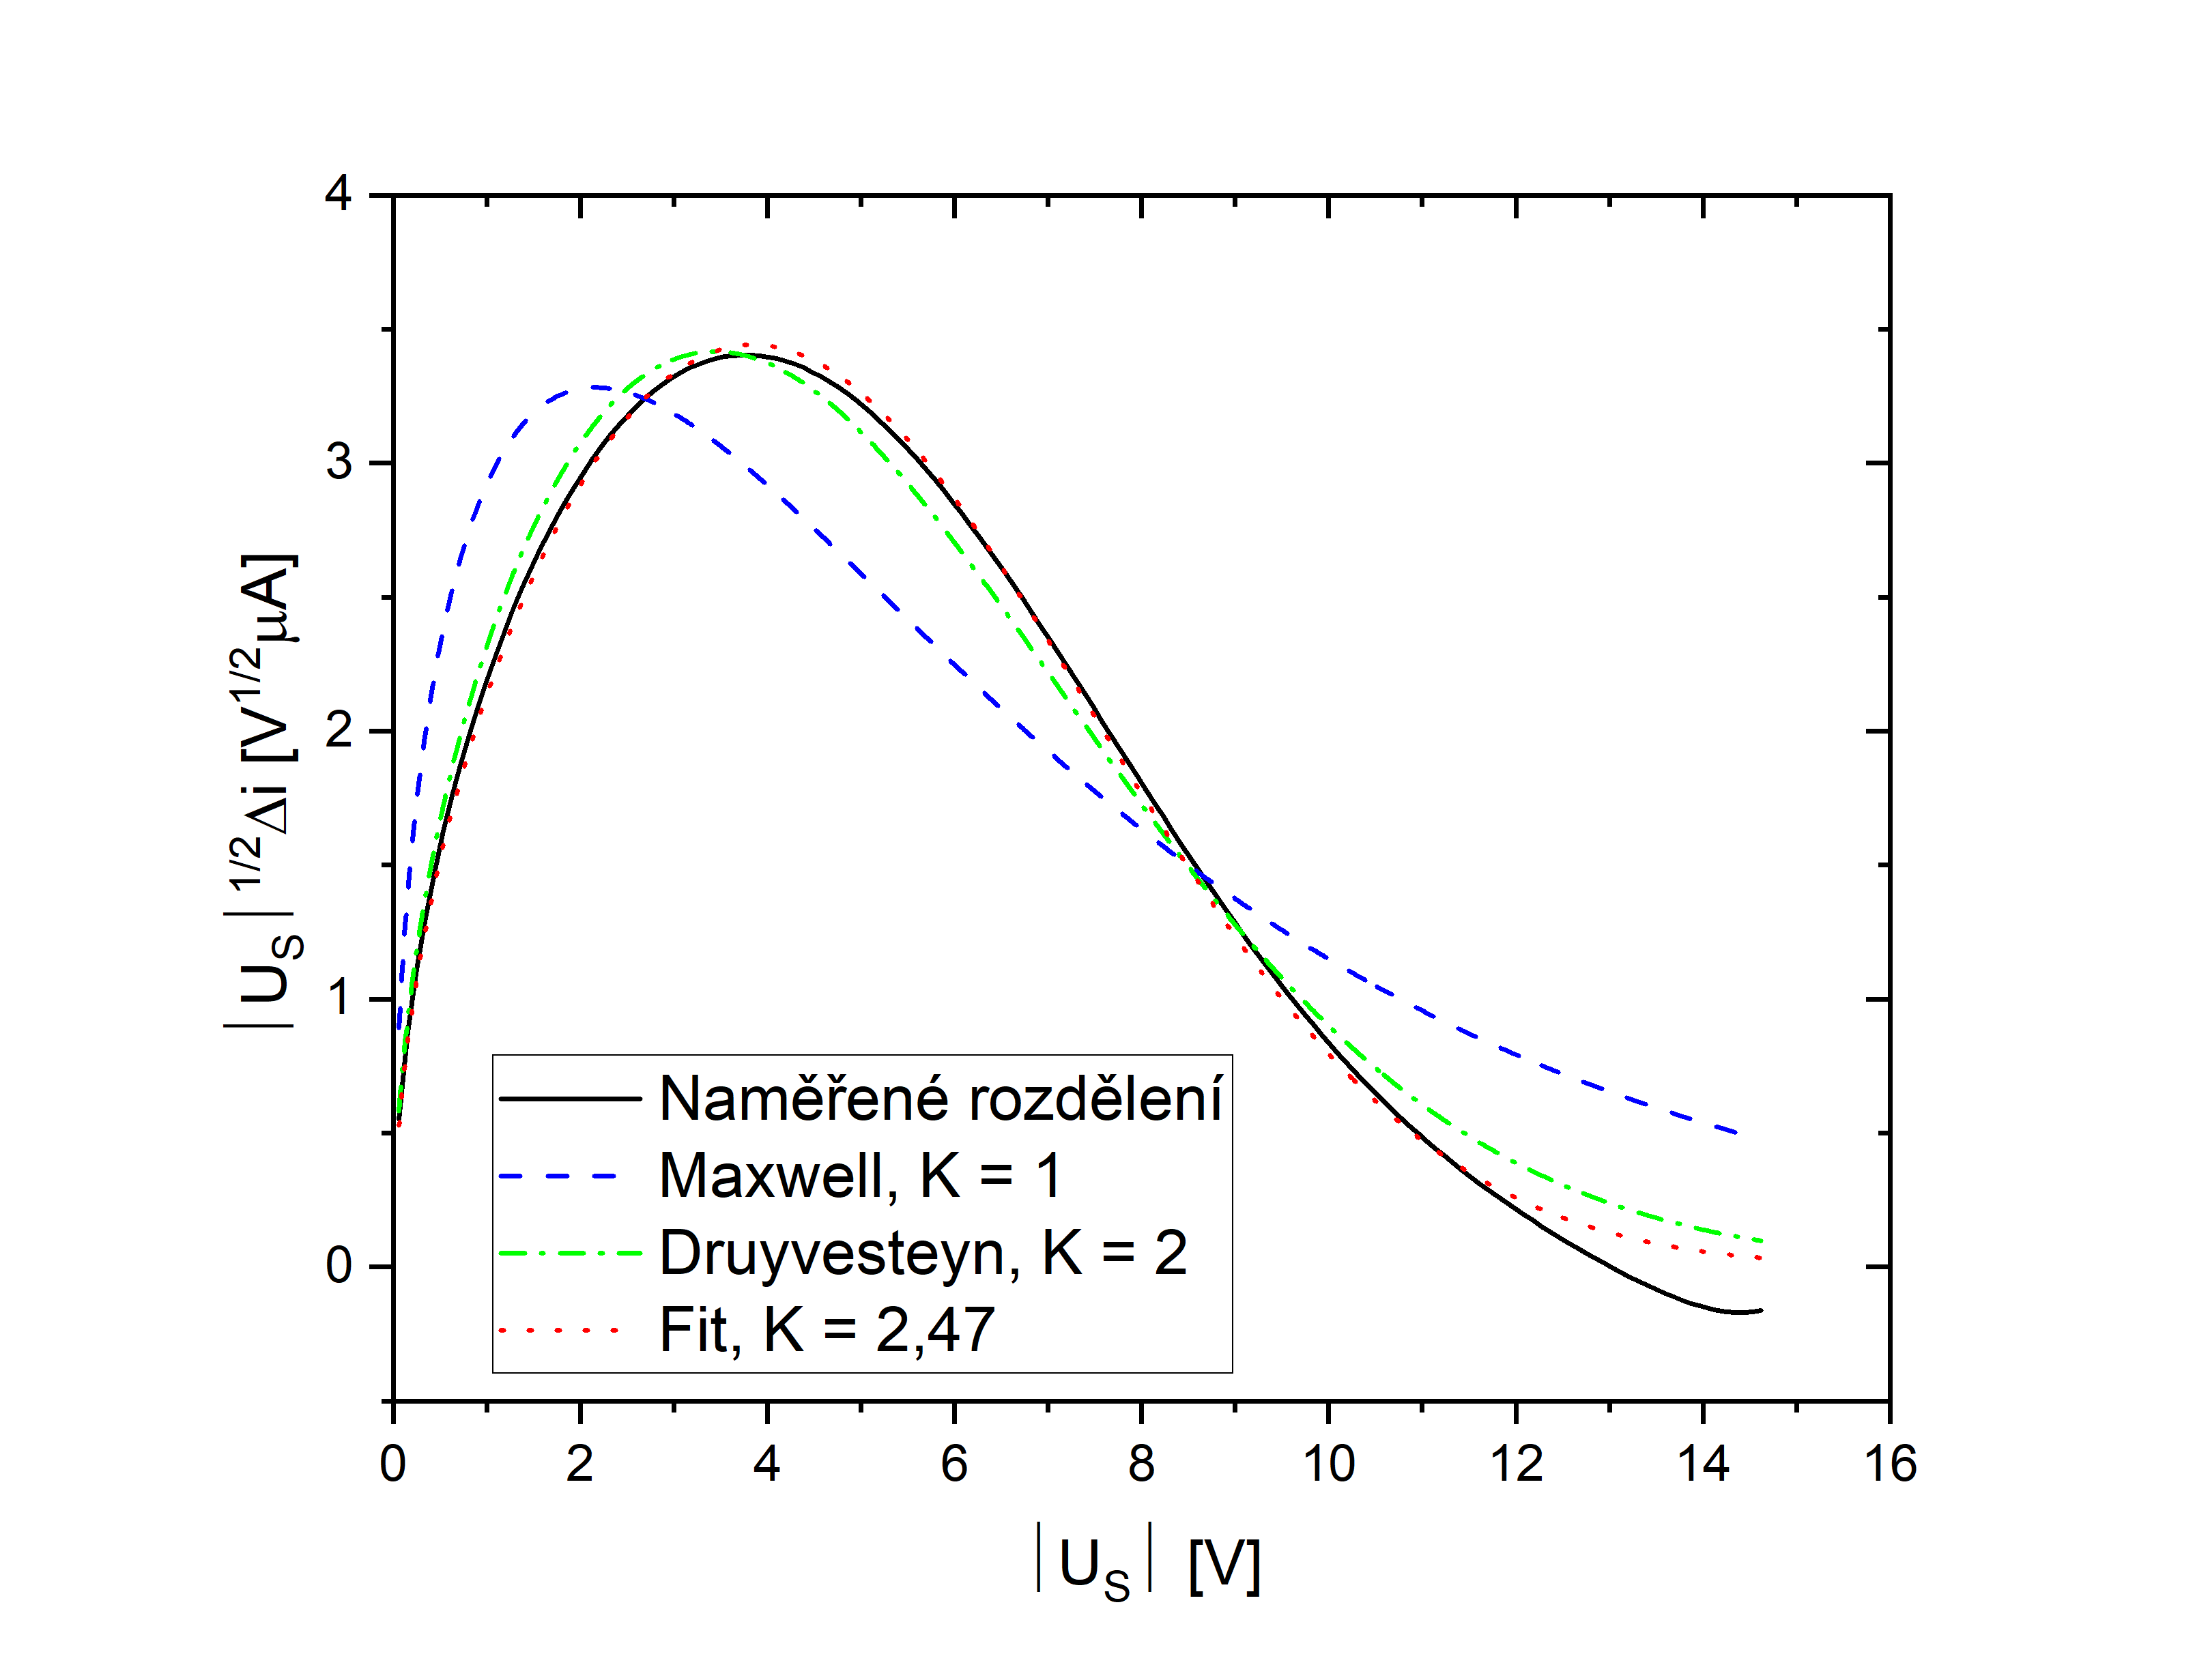
\includegraphics[width=135mm]{rozdeleniG2.png}
	\caption{Rozdělovací funkce určena metodou poruchového napětí, 
	$p=80$\,\si{\pascal}, $I_v = 30$\,\si{\milli\ampere}.}
	\label{rozdeleniG2}
\end{figure}

\begin{figure}[h!]
	\centering
	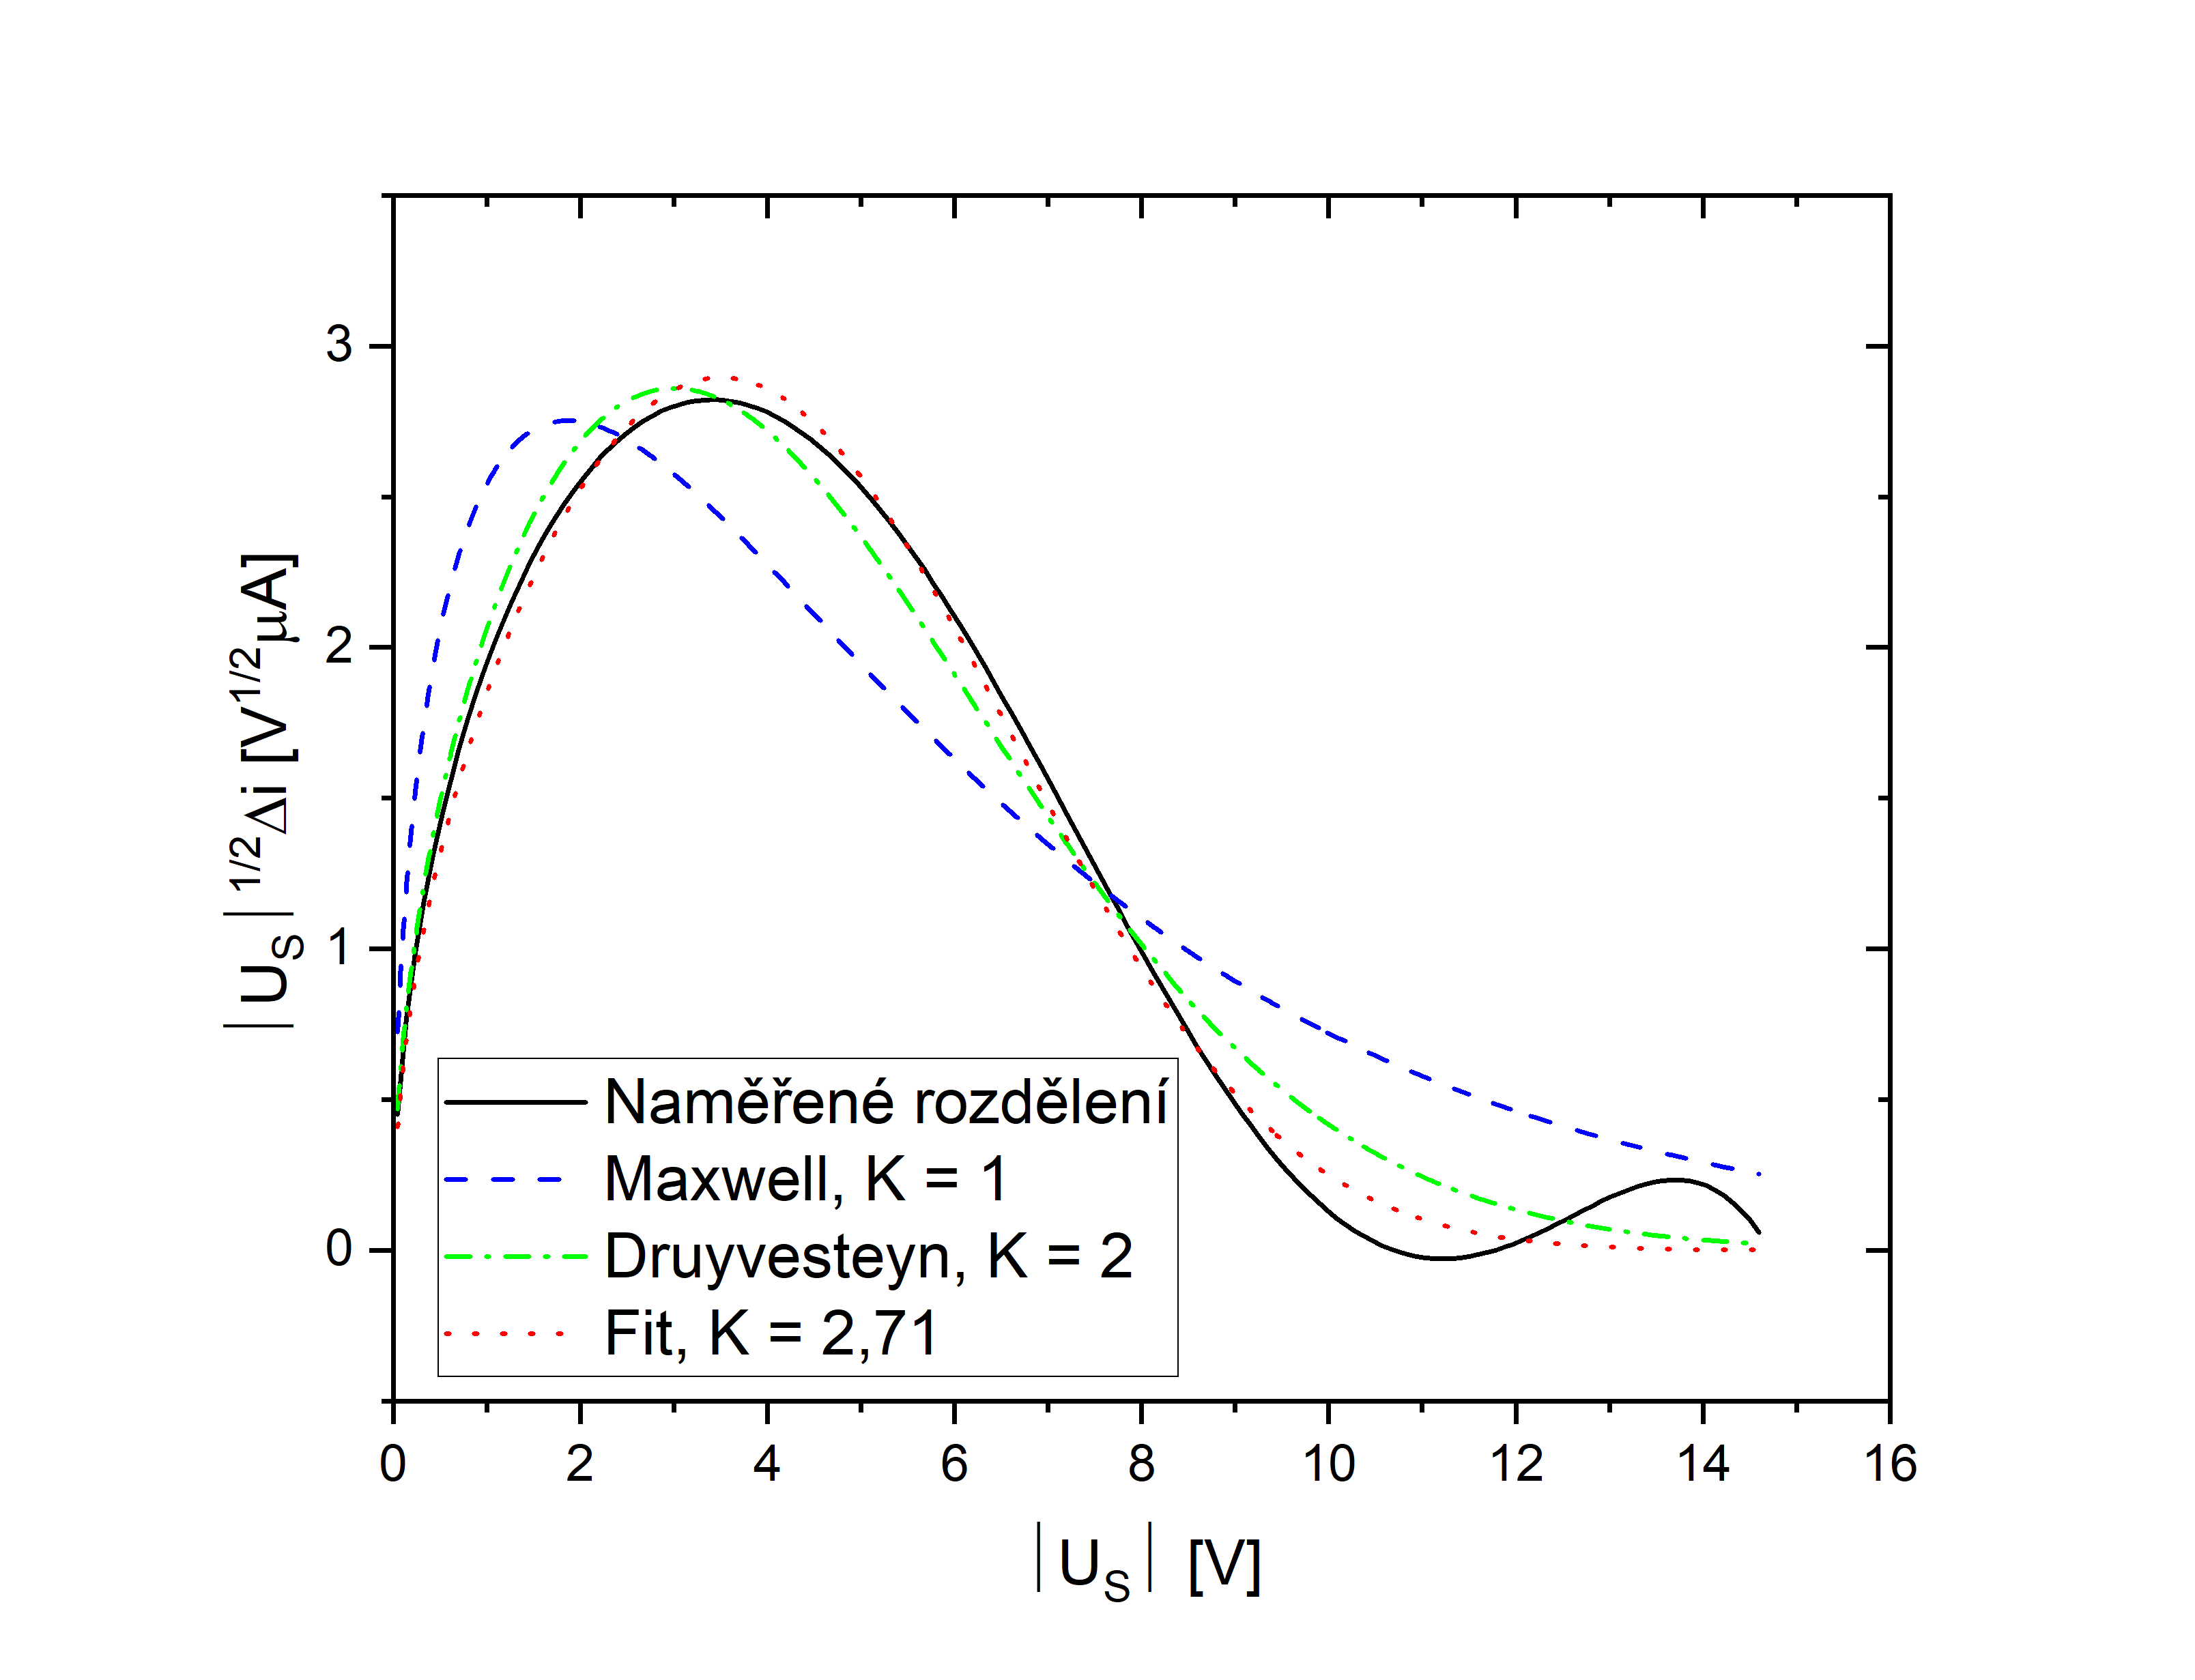
\includegraphics[width=135mm]{rozdeleniG3.png}
	\caption{Rozdělovací funkce určena metodou poruchového napětí, 
	$p=16$\,\si{\pascal}, $I_v = 55$\,\si{\milli\ampere}.}
	\label{rozdeleniG3}
\end{figure}

\begin{figure}[h!]
	\centering
	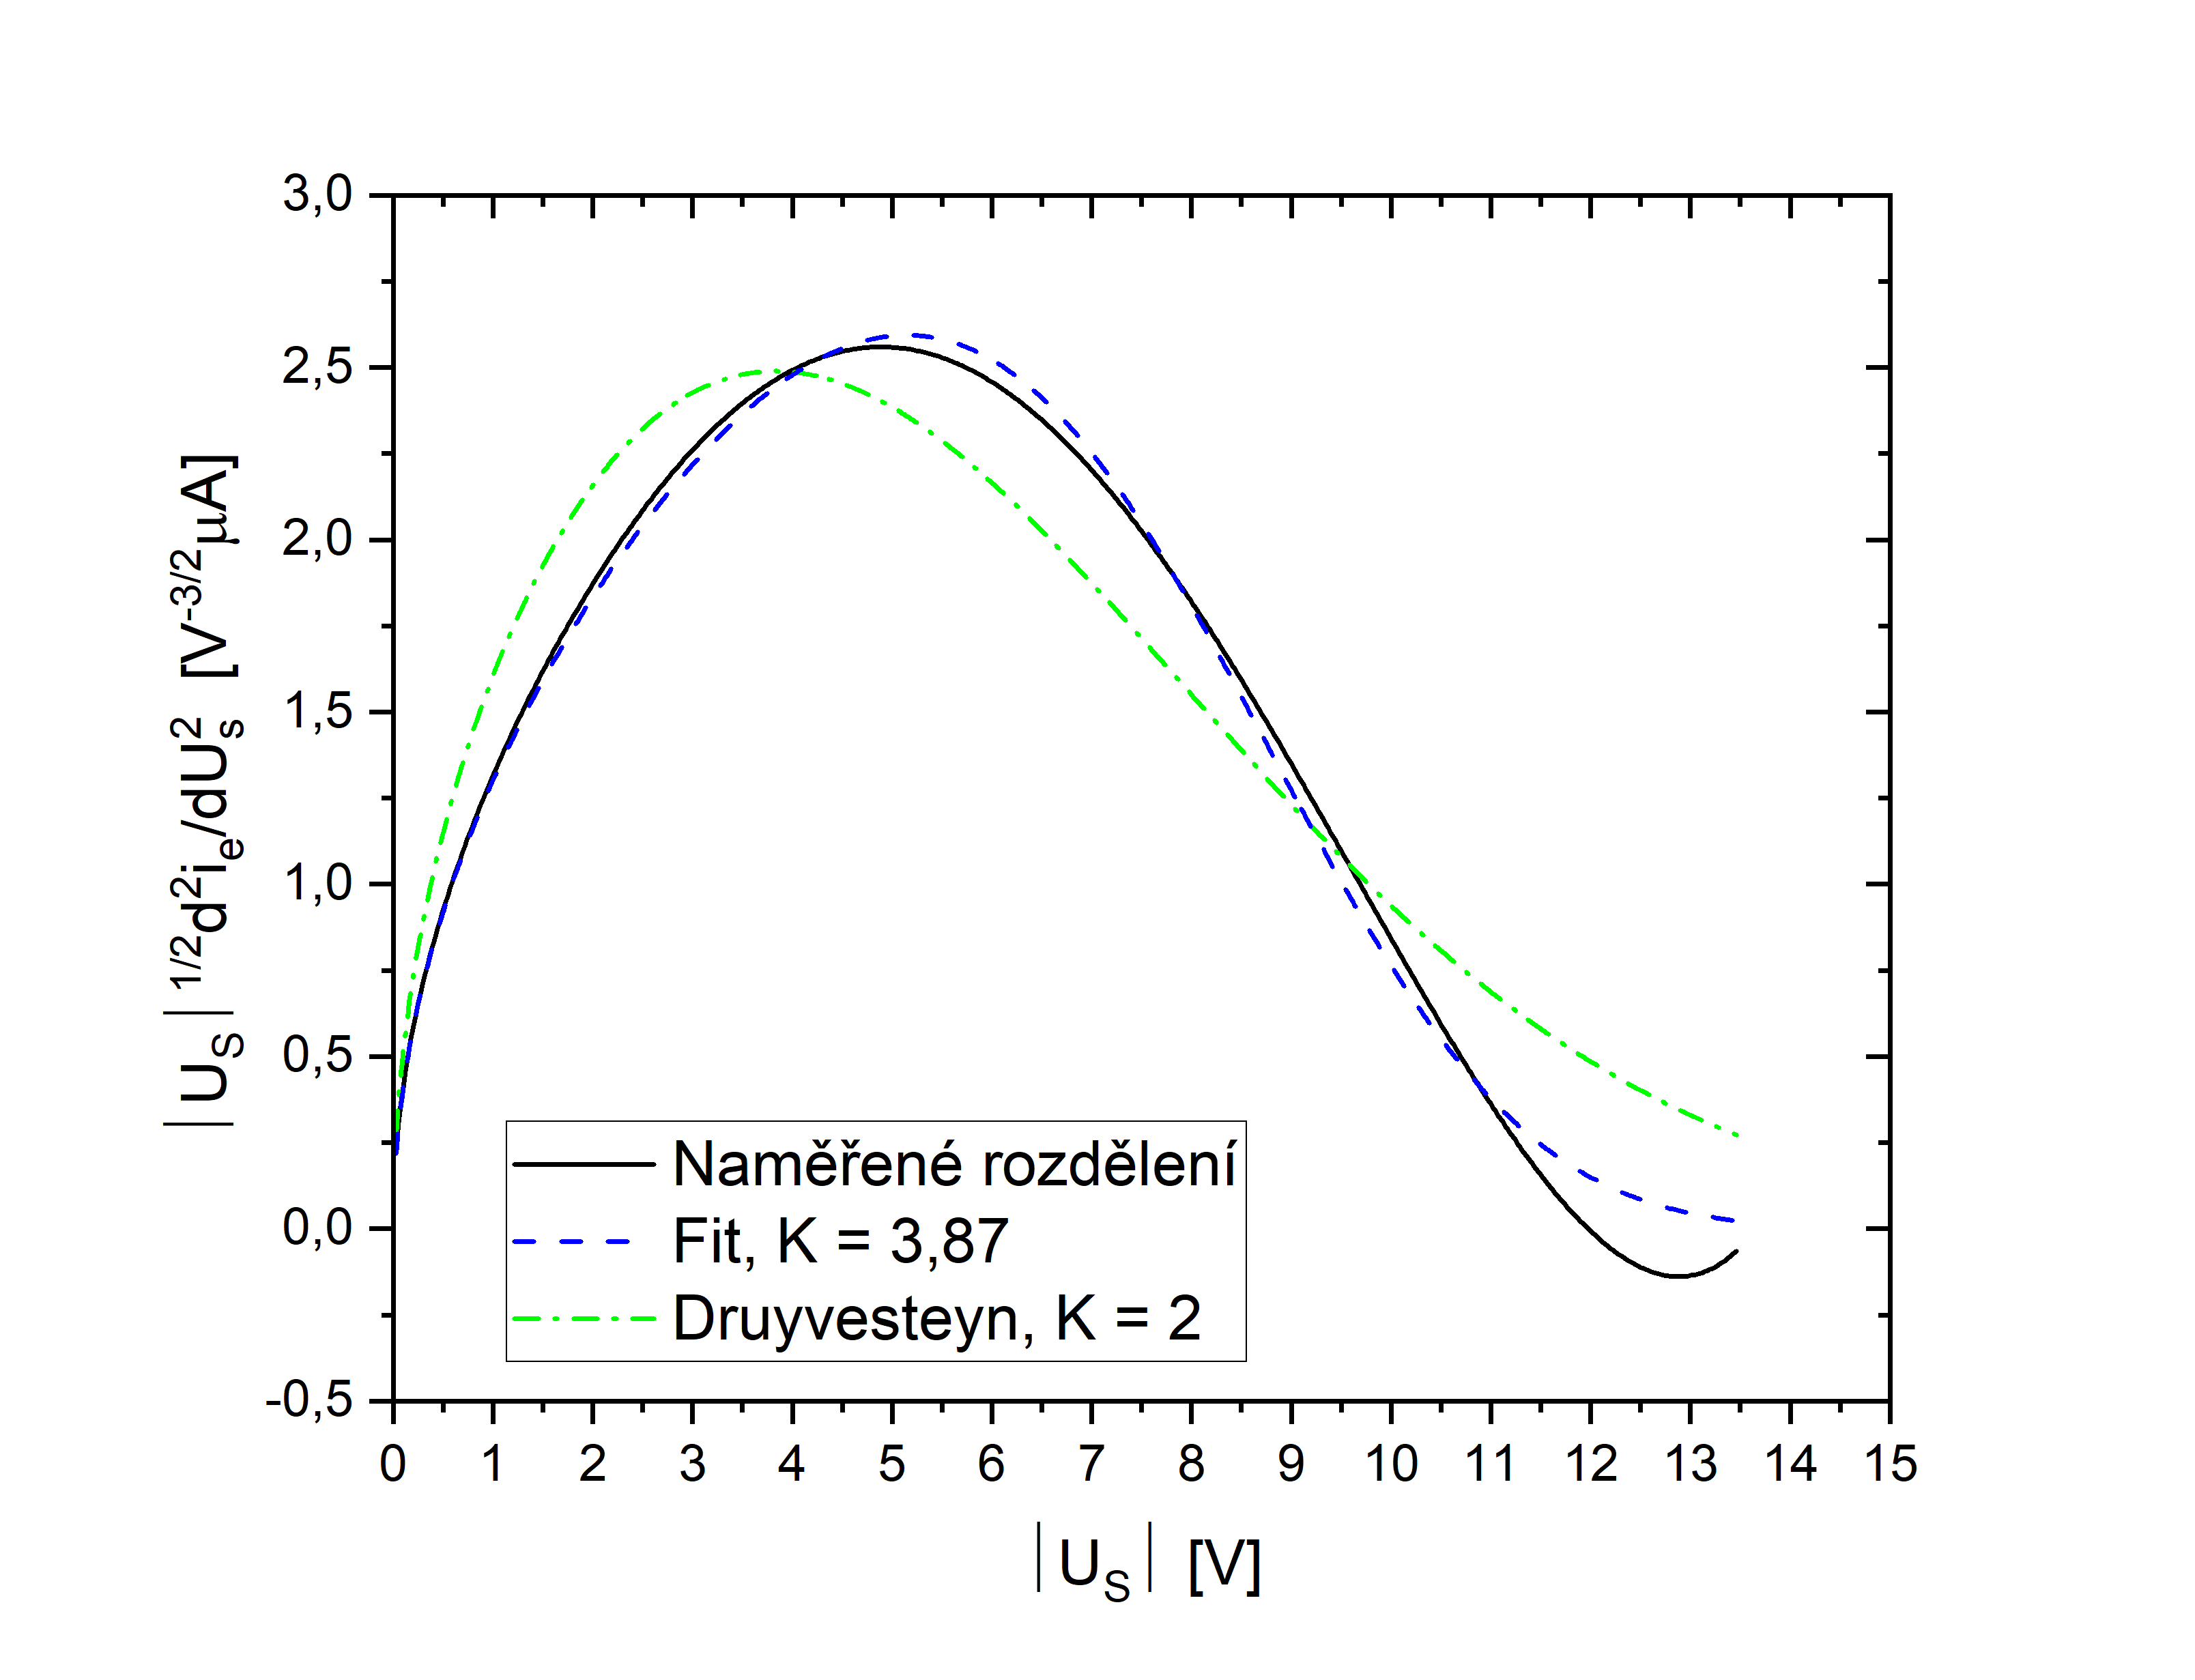
\includegraphics[width=135mm]{rozdeleniD2G1V2.png}
	\caption{Rozdělovací funkce určena metodou druhé derivace, 
		$p=80$\,\si{\pascal}, $I_v = 55$\,\si{\milli\ampere}.}
	\label{rozdeleniD2G1}
\end{figure}

\begin{figure}[h!]
	\centering
	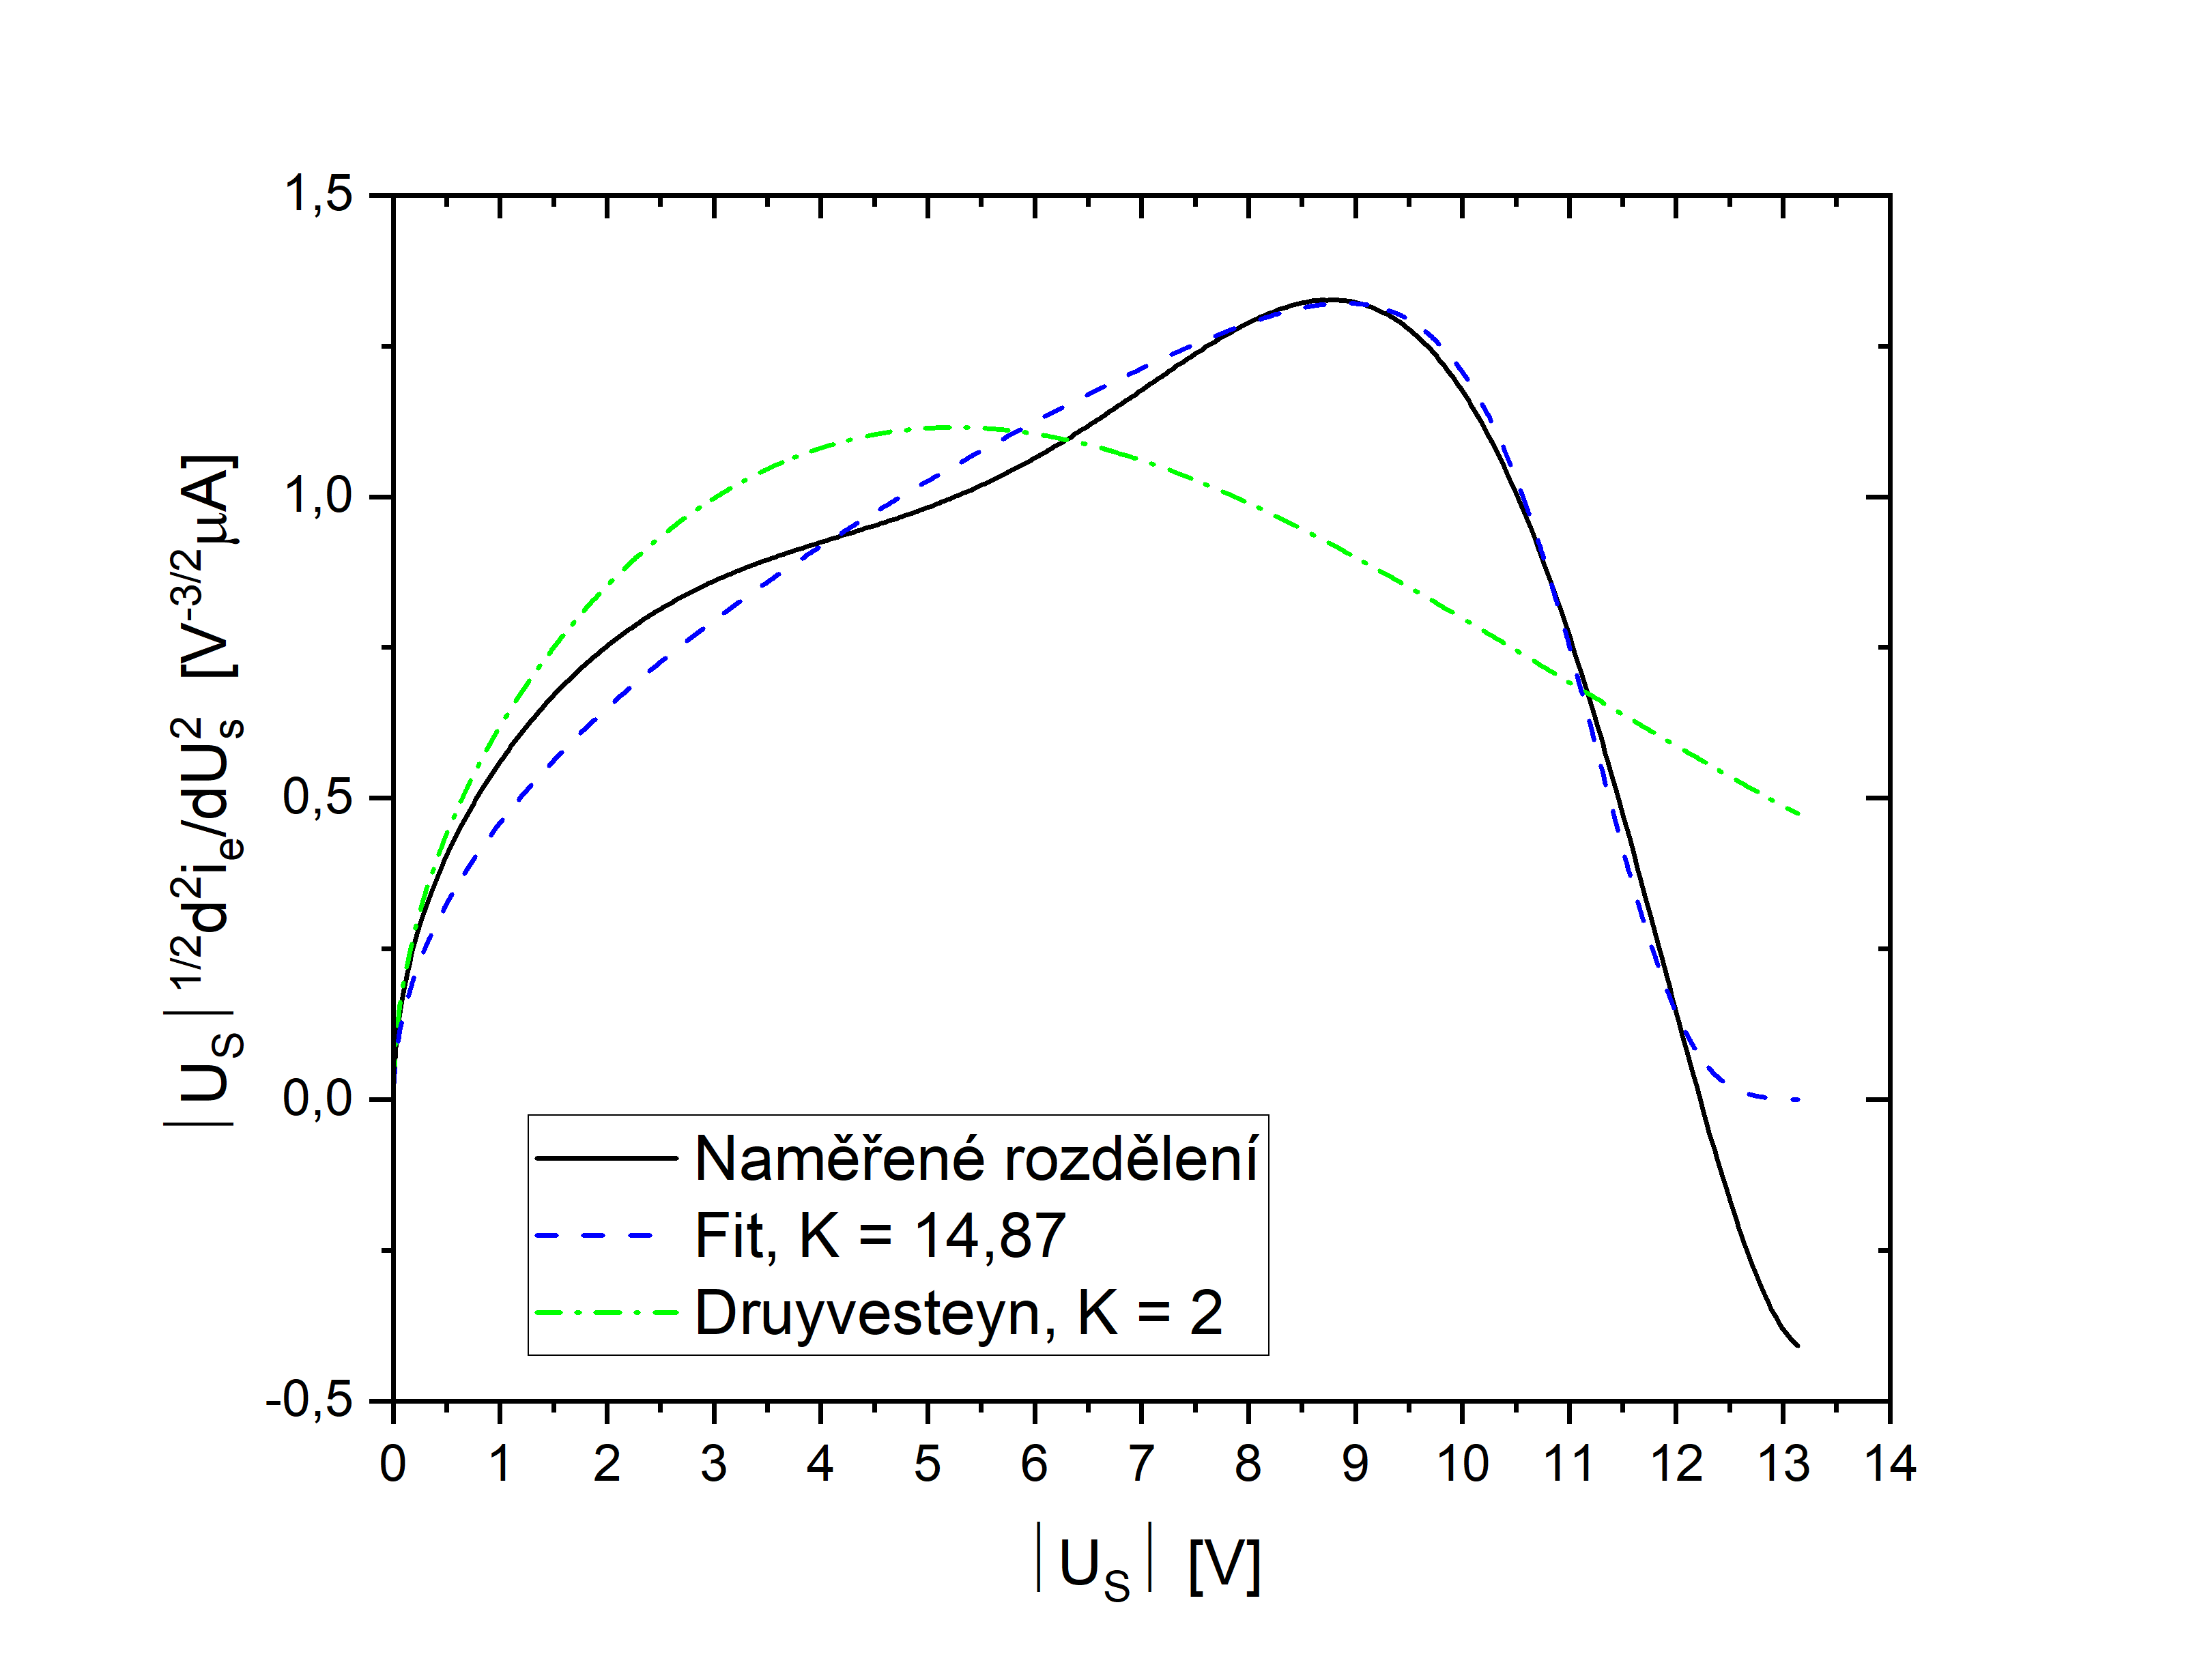
\includegraphics[width=135mm]{rozdeleniD2G2V2.png}
	\caption{Rozdělovací funkce určena metodou druhé derivace, 
		$p=80$\,\si{\pascal}, $I_v = 30$\,\si{\milli\ampere}.}
	\label{rozdeleniD2G2}
\end{figure}

\begin{figure}[h!]
	\centering
	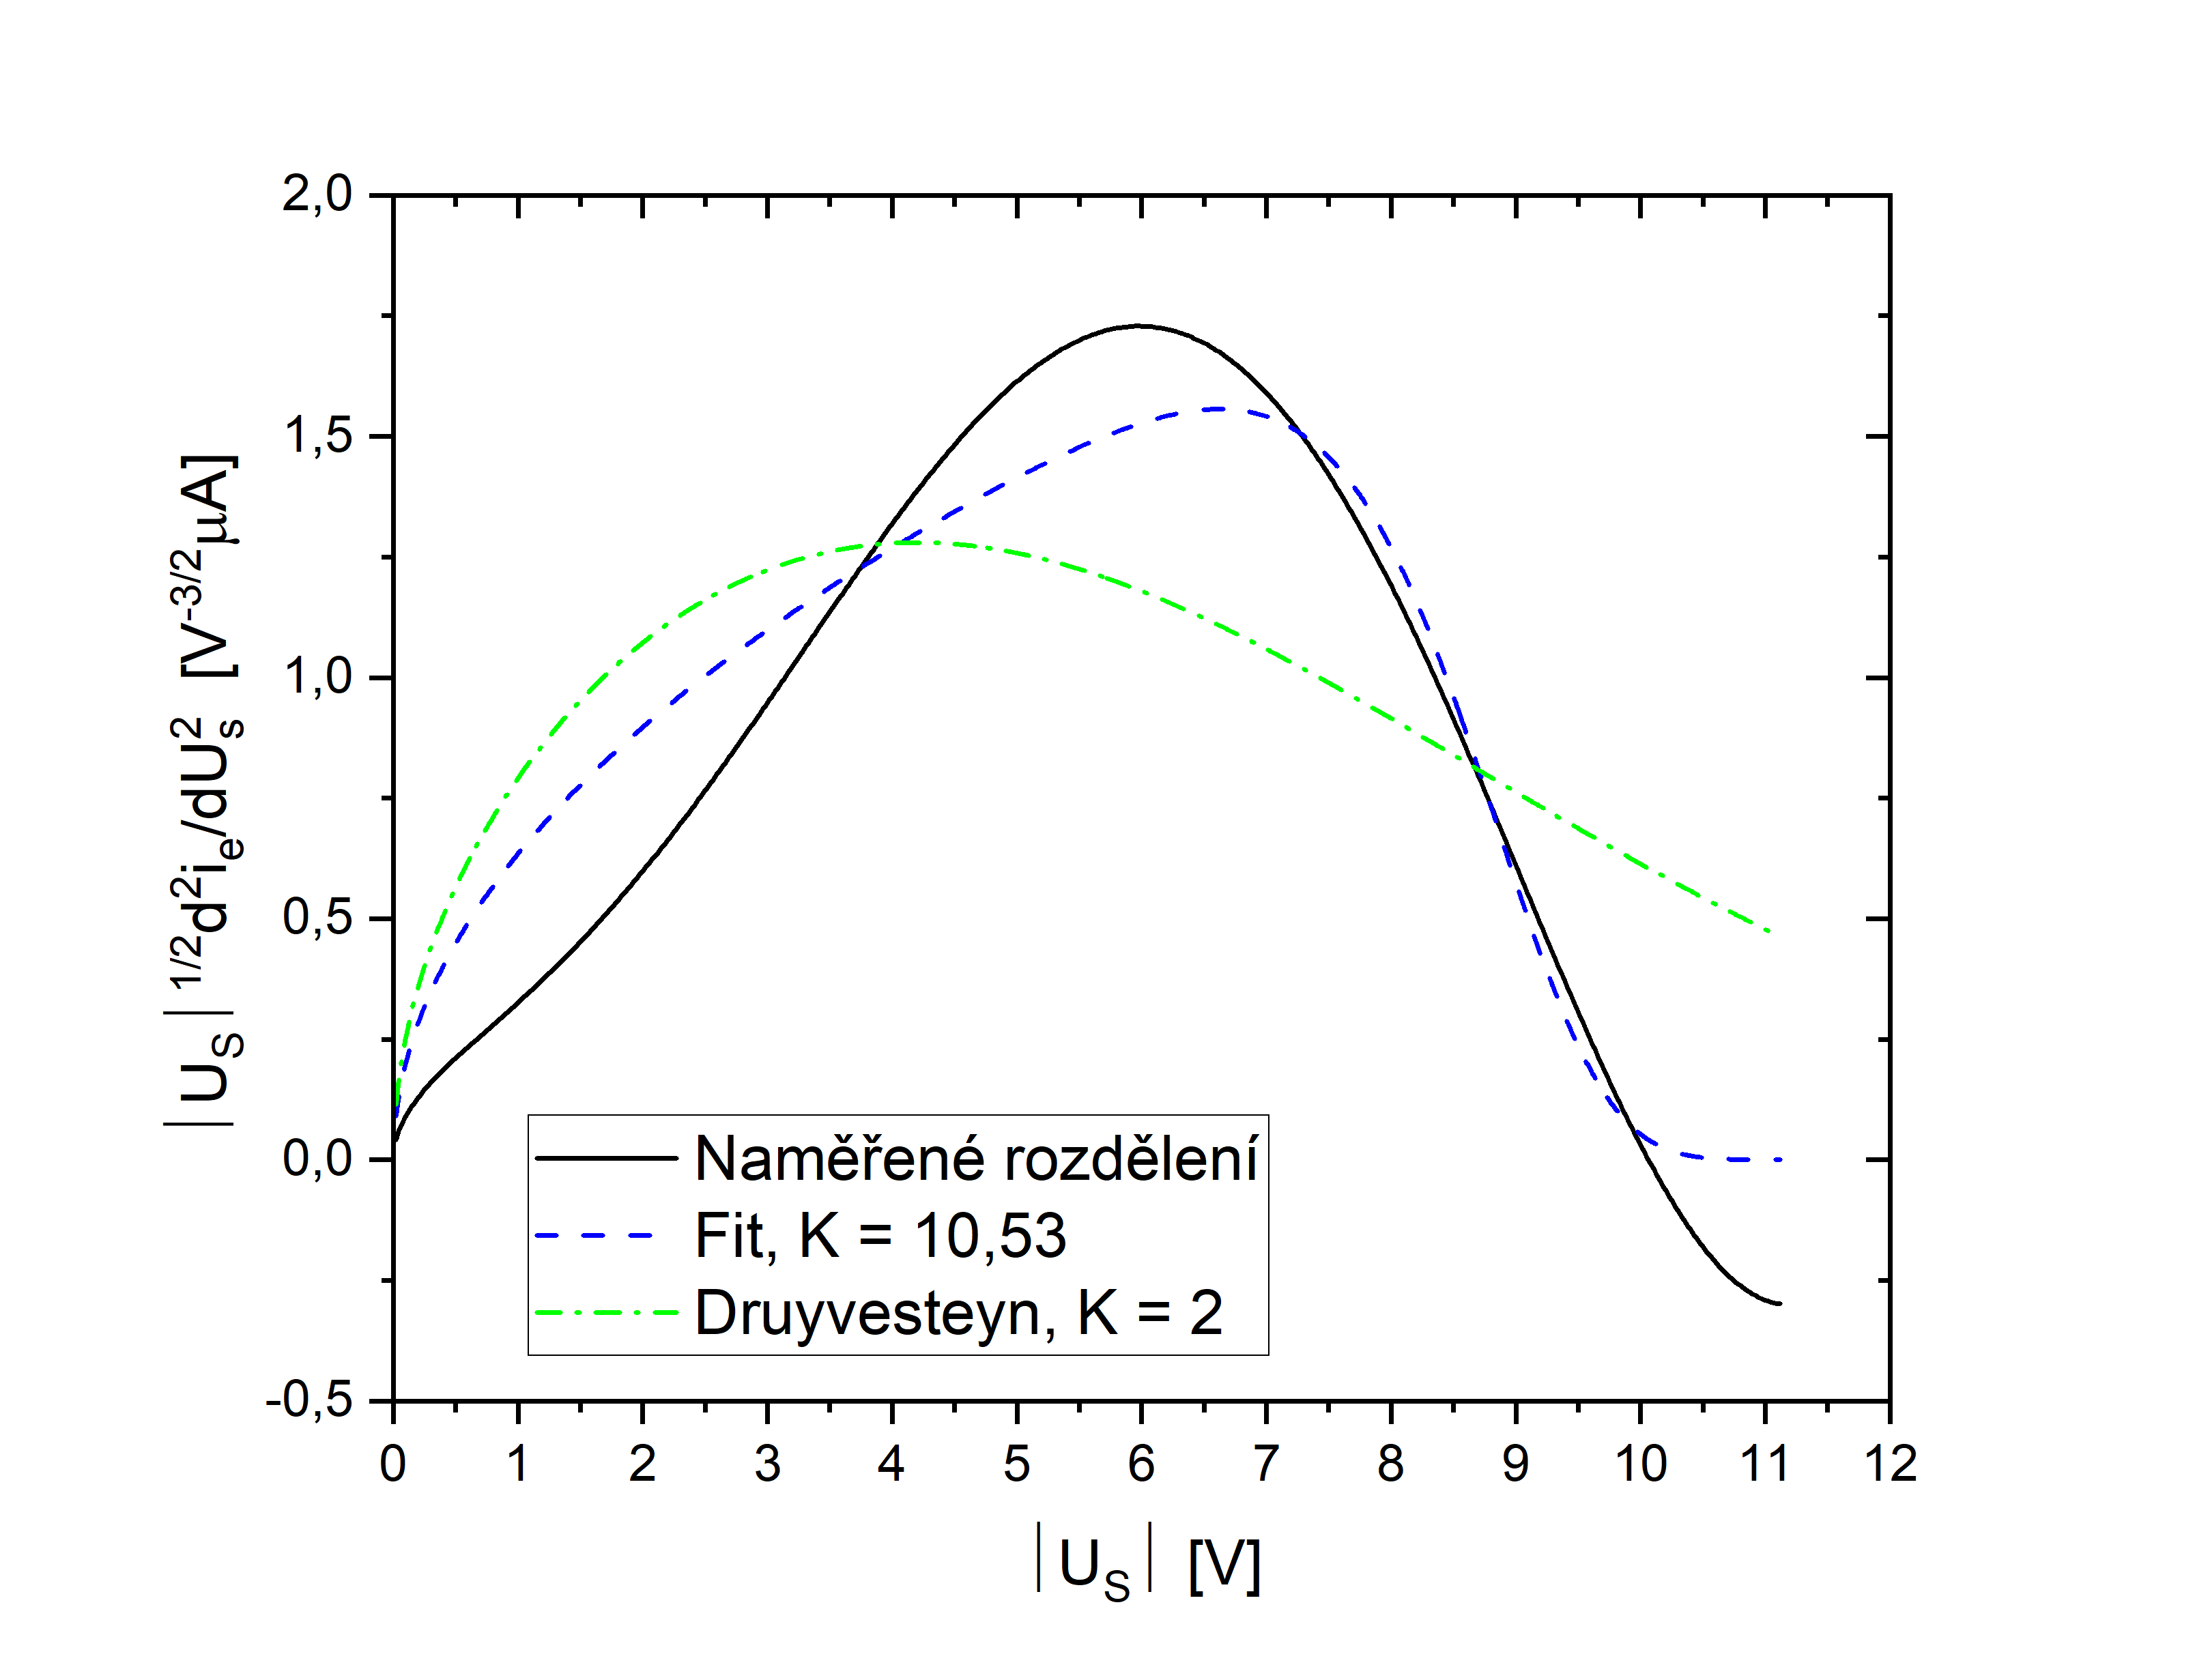
\includegraphics[width=135mm]{rozdeleniD2G3V2.png}
	\caption{Rozdělovací funkce určena metodou druhé derivace, 
		$p=16$\,\si{\pascal}, $I_v = 55$\,\si{\milli\ampere}.}
	\label{rozdeleniD2G3}
\end{figure}

\clearpage
\section{Závěr}
V této úloze jsme se seznámili s měřením pomocí Langmuirovy jednoduché válcové sondy. Naměřili jsme osm VA charakteristik pro různé
podmínky. Určili jsme plovoucí potenciál sondy, který se zvětšuje s rostoucím výbojovým proudem, při změnách tlaku za konstantního
proudu nevykazoval žádný trend. Dále jsme určili potenciál plazmatu, ten je vždy větší než plovoucí potenciál a při změnách výbojového
proudu a tlaku se chová obdobně jako plovoucí potenciál. Nakonec jsme získali elektronové teploty a spočítali elektronovou koncentraci. S rostoucím výbojovým
proudem roste i koncentrace elektronů a jejich teplota klesá. S rostoucím tlakem jsme pozorovali stejnou závislost, tedy rostoucí
koncentraci elektronů a~klesající elektronovou teplotu. Při vyhodnocování jsme 
použili dvou metod určení potenciálu plazmatu, starší metody průsečíku asymptot 
a modernější metody druhé derivace. Jejich výsledky jsou blízké.

V druhé části jsme určovali rozdělovací funkci energií. Pro vyhodnocení jsme 
použili metody poruchového napětí, výsledky metody druhé derivace jsou 
nepřesvědčivé. Zjistili jsme, že zjednodušený předpoklad 
Maxwellova rozdělení není správný, funkce odpovídá více Druyvesteynovu rozdělení. 
Pro něj platí předpoklad přítomnosti silného vnějšího elektrického pole v plazmatu
a konstantního účinného průřezu elektronů, který je nezávislý na energii.

\begin{thebibliography}{10}
	\bibitem{VA} Návod k praktiku: \textit{Diagnostika plazmatu doutnavého výboje pomocí 
	elektrostatických sond: jednoduchá sonda.}

\end{thebibliography}

\end{document}
